%%%%% FORMAT THE PAPER %%%%%%%%%%%%%%%%%%%%%%%%%%%%%%%%%%%%%%%%%%%%%%%%%%%%%%%%

%\documentclass[draft,10pt]{thesis}
\documentclass[final,12pt]{thesis}
%\documentclass[compact,10pt]{thesis}
%\documentclass[final,10pt,sflabels]{thesis}
        % Wisconsin thesis requires a single-sided printout, and the page numbers
        % should always at the up right corner ('oneside'), see thesis.cls
        % Curly brackets: Specify the "thesis" class file (thesis.cls).
        %   It assumes the existence of a few other style (*.sty) files.  
        %   See the thesis.cls file for details.
        % Square brackets, specify the options you want to use.
        %   Allowed options are 10pt, 11pt, 12pt, draft, & final.
        %   See the "thesis.cls" file for descriptions.

% NOTE: If you want your figure captions, table captions, and bibliography
% items single-spaced (this is permissible for UW theses!), you can use
% the "\fixspacing" command in each of these environments.  This command
% will choose the appropriate spacing, whether you use the "final" or
% "draft" modes.  See the "thesis.cls" class file for details.
% CLARIFICATION: The \fixspacing command has to go inside EACH of your
%     \tablenotetext blocks to be effective

%\usepackage{lscape}     % Specify this package for landscape-style tables.
% You can use this by wrapping your table in a \begin{landscape}--
% \end{landscape} environment.  Note that the rotated table will
% probably *not* show up in Xdvi, but *will* show up in the PostScript
% version (e.g., can be seen with gv).



\usepackage{xspace}
%\usepackage{longtable}   % Specify this package for multipage tables

%\usepackage[final]{graphicx}    % Use the LaTeX2e graphics package
\usepackage{graphicx}    % Use the LaTeX2e graphics package

\usepackage{subfig}   % Specify this package to create multipart figures
% with multiple files combined in a single numbered figure 
% i.e., Fig. 1(a), Fig. 1(b), etc.

\usepackage{amsmath,amssymb}  % Load the package for extended mathematical symbol set
\usepackage{amsfonts} % Provides \mathcal
%\usepackage{axodraw}  % Necessary for using the ZEUS psfigadd command
%\usepackage{placeins}
%\usepackage{caption2}
%\usepackage{epsfig}
%\usepackage{wrapfig}
\usepackage{rotating} % Provides sidewaysfigure
%\usepackage{mcite}
%\usepackage{amscd}
%\usepackage{array}
%\usepackage{multirow}
%\usepackage{supertabular}
%\usepackage{dcolumn}
\usepackage{xspace}
%\usepackage{color}
\usepackage{calc}
\usepackage{ifthen}
%\usepackage{cite} % NEED THESE???
%\usepackage{notoccite} % too

\usepackage{tikz} % feynman diagrams!
\usetikzlibrary{trees}
\usetikzlibrary{decorations.pathmorphing}
\usetikzlibrary{decorations.markings}

\newcommand{\pb}{ pb\textsuperscript{-1} }
\newcommand{\lunits}{$cm^{-2} s^{-1}$ }
\newcommand{\dsigdM}{$ \frac{d\sigma}{dM_{inv}} $ }
\newcommand{\sieie}{$ \sigma_{i \eta i \eta } $ }
\newcommand{\detain}{$ \Delta \eta _{in} $ }
\newcommand{\dphiin}{$ \Delta \phi _{in} $ }
\newcommand{\dCotTheta}{$ \Delta \cot \theta $ }
\newcommand{\pt}{$ p_{T} $ }
\newcommand{\Et}{$ E_{T} $ }
\newcommand{\DR}{$ \Delta R $ }
\newcommand{\Zg}{$ Z/ \gamma^{*} $ }
\newcommand{\Zee}{$ Z \rightarrow e^{+} e^{-} $ }
\newcommand{\qqZee}{$ q \bar{q} \rightarrow Z \rightarrow e^{+} e^{-} $ }
\newcommand{\qqZgee}{$ q \bar{q} \rightarrow Z/ \gamma^{*} \rightarrow e^{+} e^{-} $ }
\newcommand{\Zgee}{$ Z/ \gamma^{*} \rightarrow e^{+} e^{-} $ }
\newcommand{\Ztautau}{$ Z/ \gamma^{*} \rightarrow \tau^{+} \tau^{-} $ }
\newcommand{\Wenu}{$ W \rightarrow e \nu $ }
\newcommand{\Wtaunu}{$ W \rightarrow \tau \nu $ }
\newcommand{\ttbar}{$ t \bar{t} $ }

%%%%%%%%%%%%%%%%%%%%%%%%%%%%%%%%%%%%%%%%%%%%%%%%%
%
%  Common definitions
%
%  N.B. use of \providecommand rather than \newcommand means
%       that a definition is ignored if already specified
%
%  so I changed them all...
%
%%%%%%%%%%%%%%%%%%%%%%%%%%%%%%%%%%%%%%%%%%%%%%%%%

% ---------- Physics symbols
\providecommand{\pT}{\ensuremath{p_{\mathrm{T}}}\xspace}
\providecommand{\eT}{\ensuremath{E_{\mathrm{T}}}\xspace}
\providecommand{\pt}{\ensuremath{p_{\mathrm{T}}}\xspace}
\providecommand{\et}{\ensuremath{E_{\mathrm{T}}}\xspace}
\providecommand{\kt}{\ensuremath{k_t}\xspace}

\providecommand{\ppbar}{\ensuremath{{p\overline{p}}}\xspace}
\providecommand{\bbbar}{\ensuremath{{p\overline{p}}}\xspace}
\providecommand{\ttbar}{\ensuremath{{p\overline{p}}}\xspace}


% ---------- Luminosities
\providecommand{\Lllow}  {\ensuremath{\mathcal{L}=\text{10}^\text{31}\,\text{cm}^\text{$-$2}\,\text{s}^\text{$-$1}}\xspace}
\providecommand{\Llow}  {\ensuremath{\mathcal{L}=\text{10}^\text{32}\,\text{cm}^\text{$-$2}\,\text{s}^\text{$-$1}}\xspace}
\providecommand{\Lmed}  {\ensuremath{\mathcal{L}=\text{10}^\text{33}\,\text{cm}^\text{$-$2}\,\text{s}^\text{$-$1}}\xspace}
\providecommand{\Lhigh}  {\ensuremath{\mathcal{L}=\text{10}^\text{34}\,\text{cm}^\text{-2}\,\text{s}^\text{$-$1}}\xspace}

\providecommand{\pbinv} {\mbox{\ensuremath{\,\text{pb}^\text{$-$1}}}\xspace}
\providecommand{\fbinv} {\mbox{\ensuremath{\,\text{fb}^\text{$-$1}}}\xspace}
\providecommand{\lumi}{\ensuremath{\mathcal{L}}\xspace}
\providecommand{\Lumi}{\ensuremath{\mathcal{L}}\xspace}%both upper and lower

% ---------- Units
\providecommand{\MeV}{\ensuremath{\,\text{Me\hspace{-.08em}V}}\xspace}
\providecommand{\GeV}{\ensuremath{\,\text{Ge\hspace{-.08em}V}}\xspace}
\providecommand{\TeV}{\ensuremath{\,\text{Te\hspace{-.08em}V}}\xspace}
\providecommand{\mev}{\ensuremath{\,\text{Me\hspace{-.08em}V}}\xspace}
\providecommand{\gev}{\ensuremath{\,\text{Ge\hspace{-.08em}V}}\xspace}
\providecommand{\tev}{\ensuremath{\,\text{Te\hspace{-.08em}V}}\xspace}


% Define styles for the different kind of edges in a Feynman diagram
\tikzset{
%  photon/.style={decorate, decoration={snake}, draw=npurple},
%  photon/.style={decorate, decoration={snake}, draw=purple},
  photon/.style={decorate, decoration={snake}, draw=black},
%  boson/.style={decorate, decoration={snake}, draw=npurple},
%  boson/.style={decorate, decoration={snake}, draw=purple},
  boson/.style={decorate, decoration={snake}, draw=black},
%  zboson/.style={dashed, draw=black},
  zboson/.style={decorate, decoration={dash}, draw=black},
%  electron/.style={draw=jblue, postaction={decorate},
%  electron/.style={draw=blue, postaction={decorate},
  electron/.style={draw=black, postaction={decorate},
    %        decoration={markings,mark=at position .55 with {\arrow[draw=jblue]{>}}}
  },
%  fermion/.style={draw=jblue, postaction={decorate},
%  fermion/.style={draw=blue, postaction={decorate},
  fermion/.style={draw=black, postaction={decorate},
    %        decoration={markings,mark=at position .55 with {\arrow[draw=jblue]{>}}}
  },
%  gluon/.style={decorate, draw=wred,
%  gluon/.style={decorate, draw=red,
  gluon/.style={decorate, draw=black,
    decoration={coil,amplitude=4pt, segment length=6pt}} 
}



% Line numbers for drafts, thanks to Carlos P.d.l.H. from AMANDA.
% To use this feature, say \linenumbers right after \begin{document}.
% Be sure to remove before printing out the final version!
%                                       --Katherine Rawlins, Oct. 2001
%\usepackage[displaymath,mathlines]{lineno}


%\nofiles       
        % Uncomment to prevent the creation of new *.toc *.lot, and *.lof 
        %   files.  Do this if you need to edit these files for the final
        %   version of the paper.  For example, if you have multi-page 
        %   figures or tables but you want the lists of figures & tables
        %   to have only one line for these, you will need to delete the
        %   extra lines in the *.lof and *.lot files and re-run LaTeX.

%\graphicspath{{figs/}}  % Specifies a subdirectory containing graphics files
                        % Multiple directories possible, each with inner {}
                        %   within the outer {}; e.g., {{figs/}{~/plots}}


   % Use \includeonly{} if you are just working on one \include{}'d
   % section.  This prevents LaTeX from re-processing the unneeded
   % chapters, but preserves references and page/fig/table numbers.
   % Try it.  You'll like it. 
   % Default is to compile entire document.
%\includeonly{detector.tex}

%\input{define}          % Read in list of user-defined LaTeX commands
%\include{citations}
%\include{zeus_def}

\begin{document}        % BEGIN THE DOCUMENT TEXT

%  The cool linenumbers feature... comment it out for the final version
%\linenumbers



%%%%% BEGIN TITLE/CONTENTS PAGES %%%%%%%%%%%%%%%%%%%%%%%%%%%%%%%%%%%%%%%%%%%%%%

\mytitle{
Z boson cross section measurement using CMS at the LHC
}
\myauthor{Jessica Lynn Leonard}
\myyear{2011}

% These aren't really needed except for the UMI abstract
\adviser{Wesley H. Smith}
\adviserrank{Professor}

\ttlpage                % This command produces the title page.  Nifty!
\cpypage                % This produces the copyright page.  Also nifty!
                        % Reminder: it costs money to retain copyright
                        
% The following three lines are for UMI abstract only
                        % Reminder: UMI abstract is required by gradschool but it is NOT a part of your thesis
%\begin{umiabstract}
%\input{umiabstract}    % *.tex file for UMI abstract page
%\end{umiabstract}      % Need to use \input rather than \include to avoid
                        %  implicit \clearpage's.  You shouldn't have any
                        %  cross-references between abstract and text, so
                        %  \input should be OK.

\frontmatter            % Choose roman-type numbers; reset page numbers to 1.

\pagestyle{thesis}      % Set the page style to "thesis" 
                        %   (page numbers at the top right)

%%%%% BEGIN ABSTRACT ETC. %%%%%%%%%%%%%%%%%%%%%%%%%%%%%%%%%%%%%%%%%%%%%%%%%%%%%
%% \begin {abstract}

%% \noindent Inclusive dijet and trijet production in deep inelastic $ep$ scattering has been
%% measured for $10<Q^2<100$ GeV$^2$ and low Bjorken $x$,
%% $10^{-4}<x_{\rm Bj}<10^{-2}$.  The data were taken at the HERA $ep$ collider
%% with center-of-mass energy $\sqrt{s} = 318$ GeV using the ZEUS detector
%% and correspond to an integrated luminosity of $82~{\rm pb}^{-1}$.  Jets were
%% identified in the hadronic center-of-mass (HCM) frame using the $k_{T}$ cluster
%% algorithm in the longitudinally invariant inclusive mode.  Measurements of dijet and
%% trijet
%% differential cross sections are presented as functions of $Q^2$, $x_{\rm Bj}$, jet
%% transverse energy, and jet pseudorapidity.  As a further examination of low-$x_{\rm Bj}$ dynamics,
%% multi-differential cross sections as functions of the jet correlations in transverse
%% momenta,
%% azimuthal angles, and pseudorapidity are also presented.  Calculations at $\mathcal{O}(\alpha_{s}^3)$ generally
%% describe the trijet data well and improve the description of the dijet data compared
%% to the
%% calculation at $\mathcal{O}(\alpha_{s}^2)$.

\noindent The cross section of 
$p p \rightarrow Z \rightarrow e^+ e^-$ 
was measured for $\sqrt{s} = 7$ TeV $pp$ collisions 
at the Large Hadron Collider using the 
Compact Muon Solenoid detector.  
Well-reconstructed electrons within the region 
$ |\eta| < 1.4442, 1.566 < |\eta| < 2.5$ 
and with a transverse energy of at least 25 GeV 
were used, 
with an invariant mass window of 60 to 120 GeV.  
In 36.1 \pb of data, 8453 candidate events were found.  
The cross section was measured to be 
990 $\pm$ 48 pb, 
which agrees well with the NNLO prediction 
of 972 pb.  

\end{abstract}
      % *.tex file for abstract
%% %\include{sponsor}      % *.tex file for "sponsorship" page
%% %\include{dedicate}     % *.tex file for dedication
%% %\include{quotes}       % *.tex file for quotations
%% \begin{acknow}
%ACKNOWLEDGEMENTS HERE

I would like to thank the professors 
who have mentored and advised me 
during my time as a grad student, 
Wesley Smith and Sridhara Dasu, 
as well as the scientists I have worked with 
over the years: 
Pam Klabbers, Sascha Savin, and Monika Grothe.  
I would also like to thank my fellow CMS students 
for their camaraderie and willingness to share knowledge, 
and my friends in Madison and in Geneva 
for providing a social outlet and a listening ear.  

Finally, I would like to thank my family, 
who never stopped encouraging me 
throughout this journey.  

\end{acknow}
   % *.tex file for acknowledgements

\tableofcontents        % *.toc file with table of contents
\listoffigures          % *.lof file with list of figures   % SWITCHED
\listoftables           % *.lot file with list of tables    % THESE TWO
     % Note that the \listoftables does not play well with the
     % deluxetable environment.  You will probably have to do some
     % hand-tweaking of the master.lot file if you have multi-page
     % tables. 
\clearpage
\pagebreak              % Enforce the start of a new page


%\prelimpages % from the UWash template -- what does it do?



%%%%% BEGIN TEXT OF PAPER %%%%%%%%%%%%%%%%%%%%%%%%%%%%%%%%%%%%%%%%%%%%%%%%%%%%%

\mainmatter

%\setfoot{\small \itshape \centerline{ DRAFT \today }} 

% This is a hand-tweak by Dolan to fix his odd landscape tables in
% compact style.  REMOVE THIS for your thesis!
%\ifkompakt\renewcommand\arraystretch{1.1}\else\fi

%\textpages  % UWash thesis template has this, what is it?

%\include{chapter_1_intro}                % *.tex file for the Introduction
%\include{chapter_2_evolution}                % *.tex file for the Introduction
%\include{chapter_3_detector}      
%\include{chapter_4_LO_MC}
%\include{chapter_5_NLO}
%\include{chapter_6_reconstruction}
%\include{chapter_7_selection}
%\include{chapter_8_analysis}   
%\include{chapter_9_results}
%\include{chapter_10_conclusion}    % *.tex file for the Conclusion

\chapter{Overview}
\label{over}

%Little intro thing about science and stuff -- my story?

It is natural for humans to wonder how the world works.  % ``people''? ``how things work''?
Small children commonly ask a plethora of questions, 
sometimes pushing their parents to the point of exasperation.  
% quote on curiosity or someting?
I was one such child, always asking questions, and later %, 
devouring books and magazines, with a hunger to learn more.  
My first exposure to particle physics came at age eleven 
when I discovered my parents' copy of 
\textit{A Brief History of Time} by Stephen Hawking.  % REFERENCE
The ideas described therein -- fundamental particles 
with exotic properties, the flexible nature of spacetime, 
what might lie beyond the edges of our understanding -- 
boggled my mind, and I loved it.  
Over the following years I checked out much of the 
local library's collection of popular physics books.  
It is this desire to know more about the fundamental 
nature of the universe that has brought me to the point 
of pursuing a doctorate in experimental particle physics.  

%History
%short history of particle physics?
%quantum mech, cosmic ray detection with bubble chambers, etc, 
%first seeing the Z
%move on to accelerators
%talk a little about proton interactions, 

%maybe have all this history and the random definitions together 

\section{Short Overview of Particle Physics}
This hunger to figure out how things work has long 
been a part of human life.  
One of the most lasting questions has been 
``What, exactly, are things made of?'' 
%ancient greeks
The ancient Greeks tried to distill all matter into % DO I NEED TO REFERENCE ALL THE HISORICAL STUFF?  it came from wikipedia, and I would think it's common knowledge
four elements: fire, earth, water, and air.  % look up role of quintessence
They also came up with the idea of an ``atom,'' 
the smallest possible piece of matter, 
a piece that could be divided no further.  
%%galileo etc 
%In the Middle Ages, astronomers such as 
%Copernicus, Kepler, and Galileo 
%tried to formulate a system to 
%describe the motions of the heavenly bodies. 
%%enlightenment
%%newton
%Isaac Newton's laws of motion and gravitation %, 
%in the 17th and 18th centuries began the 
%``modern'' period of physics research.  
%They are still 
%recognized as valid in a wide physical context 
%and form the starting point for many 
%of today's introductory physics courses.  
%%1800's, maxwell
%Experimentation with electricity in the 18th and 
%19th centuries led to the first ``unification'' of forces: 
%James Maxwell's description of electricity and magnetism 
%in the same mathematical framework.   
%%early atom stuffs
%At this point research turned from phenomena 
%experienced in everyday life (magnets, gravity, motion) 
%to more esoteric effects.  
%% ADDED
%During the Middle Ages,
%Alchemists during the Middle Ages 
%recognized 
Natural philosophers through the ages 
discovered various chemical elements.  
However, not until relatively recently was 
the concept of the atom accepted scientifically. %, 
Up until the late 19th century, 
the issue was still debated.  
Dmitri Mendeleev's organization of the elements 
into a table according to the similarity of their properties 
hinted at an underlying structure.  
In addition, an atomic theory explained certain 
features of the behavior of gases, 
as applied by Ludwig Boltzmann and 
Amedeo Avogadro.  
However, the issue was not fully settled until 
the beginning of the 20th century.  
%This was when 
During this period 
Albert Einstein used an atomic theory of matter 
to explain the random motion of particles in a fluid %, 
(called Brownian motion after Robert Brown, who first observed it), 
and Jean Perrin verified the theory experimentally.  
Around this time progress was also being made 
on investigations into the structure of the atom.  
%% END ADDED
J.J. Thomson discovered that the cathode rays 
he was working with were 
made up of light, negatively-charged particles, 
dubbed electrons.  
He believed that these particles formed atoms, 
electrons floating in a sea of positive charge 
so that the overall element was electrically neutral: %.  
%This was 
the so-called ``plum pudding model.''  
However, experiments by Ernest Rutherford 
shooting positively-charged 
alpha particles at a sheet of gold foil demonstrated 
that the atom included a hard, positively-charged nucleus, 
illustrated in Figure~\ref{fig:AtomicModels}.  
This led 
%Ernest 
Rutherford to propose the 
planetary model of the atom, in which the positive nucleus 
is orbited by a cloud of negative electrons.  
The model did not explain why the electrons did not 
lose energy and fall into the nucleus, though; 
this explanation came when Niels Bohr applied a 
quantized idea of energy to the atom.  
The quantum theory of light, 
proposed by Max Planck and Albert Einstein, 
said that light existed in packets of a given energy, 
known as quanta. 
%Essentially, 
Applied to the atom, it meant that 
electrons were only permitted to possess 
energy and angular momentum in discrete steps.  
They moved between these energy levels by absorbing 
or emitting light of specific energies.  
%Albert Einstein's special theory of relativity took on 
%motion at speeds approaching that of light, 
%while his later theory of general relativity 
%described gravity in terms of acceleration.  
%The scientific conception of the atom progressed from 
%a positive nucleus in a cloud of negative charge 
%to a nucleus being orbited by electrons 
%in a set of specific energy states.  
%more detailed modern stuff: 40's, 50's, etc -- quarks, strange, muon, W and Z. 
Rutherford later noticed that the atomic masses 
were roughly integer multiples of the hydrogen mass; 
he proposed that atomic nuclei were made of 
positively-charged protons, 
and later added electrically neutral neutrons 
to make up the needed leftover mass.  
Meanwhile, quantum mechanics was soon formulated to describe 
the properties of particles' behavior in terms of waves 
of quantized energy.  
%The study of these fundamental particles took off 
%%during this time period, 
%after this, 
%with the proposal of a relativistic quantum theory %, 
%and the discovery of antimatter and the muon.  
Paul Dirac formulated a quantum theory that was consistent 
with Einstein's special relativity, 
which dealt with motion at speeds approaching that of light.  
In addition, the idea of forces being mediated by the exchange 
of force particles was gaining traction: 
quantum electrodynamics formulated the electromagnetic force 
as the interaction between charged particles and photons, 
or particles of light.  
%The force holding protons and neutrons together in the atomic 
%nucleus was posited to be mediated by another particle, 
%called the pion.  
At this point many new particles were being discovered, 
including the pion, 
such 
%as well 
as the positron and the muon, 
along with a large number of heavier particles.  
Quarks were proposed in Murray Gell-Mann's ``Eightfold Way'' 
to explain the many new heavy particles 
being found. % 
The quark model successfully explained the 
properties of neutrons and protons: 
those particles along with some of the new discoveries 
were ``baryons,'' made up of three quarks, 
while other new particles were ``mesons,'' 
made up of a quark and an anti-quark.  
The force between the quarks was the same one 
keeping the protons and neutrons together inside the 
atomic nucleus, 
mediated by particles called gluons.  
Since it was strong enough to overcome the repulsion 
between the positively-charged protons, 
it was called the strong force.  
%and were later verified experimentally.  
%The decay of the neutron and the observation of neutrinos 
%interacting with electrons necessitated 
Another force, called the weak force, 
was known to be responsible for the decay of 
neutrons into protons.  
Through the development of modern particle theory, 
it was predicted that heavy particles mediated this force.  
The discoveries of these particles, the W and the Z bosons, 
marked a success for the current theory: 
it had predicted particles that had previously been 
undiscovered.  

 \begin{figure}[htb]
  \begin{center}
    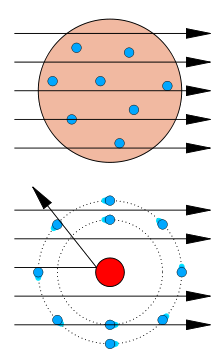
\includegraphics[width=120pt]{Figures/overview-220px-Gold_foil_experiment_conclusions_svg-opaque.png}
  \end{center}
  \caption[\fixspacing The ``plum-pudding'' and the planetary atomic models. ]
	  {\fixspacing The ``plum-pudding'' and the planetary atomic models. 
	    Observations showed incident particles back-scattering 
	    consistent with the dense, positive nucleus of 
	    the planetary model. 
	  }
  \label{fig:AtomicModels}
 \end{figure}



%recent accelerators: top. higgs and beyond...
Experiments making all these particle discoveries 
have progressed from observing cosmic rays 
in cloud chambers and bubble chambers 
to observing collisions created in higher- and higher-energy 
accelerators 
(hence the current name of the field, 
``high-energy physics'').  
Most recently, the last of the six quarks, the top quark, 
was discovered at the Tevatron accelerator in 1995 
\cite{topD0} \cite{topCDF}.  
All these particles and their interactions are described 
within the framework of the Standard Model of particle physics; 
the Standard Model combines the quantum electrodynamics 
of charged particles and photons, the quark and gluon model, 
called quantum chromodynamics, 
and the interactions of the weak force into one framework.  
%(The Standard Model, including the full set of particles 
%and their interactions, will be more fully 
%developed in Ch.~\ref{theory}.) 
The Standard Model will be further explained in 
in Chapter~\ref{theory}. 
Currently, the Standard Model is considered to be the 
primary description of particle physics.  
However, it predicts one particle that has not yet been 
observed, the Higgs boson.  
Finding the Higgs and verifying this last piece 
of the Standard Model 
is one of the current goals of 
particle physics.  
However, there are observations that 
the Standard Model cannot explain, 
such as the fact that neutrinos have mass.  
The Standard Model is also incomplete in that 
it does not incorporate the last fundamental force, gravity.  
Further, some physicists think that various additions 
to the Standard Model make it more elegant.  
These new models predict various new particles.  
Therefore, scientists are also on the lookout 
for any evidence of particle physics existing 
outside the Standard Model.  
%One particle predicted by the Standard Model has not yet 
%been discovered, the Higgs boson; 

%   * particles?  although that's theory intro (but need SOME particle-specific stuff) 
%ref ch 2 -- or wherever end up putting standard model section, maybe move to ch 1!
%some kind of short little intro, motivate need to define those following terms,
%want to talk about Z and why important, motivations


%   * ``high-energy''
%``High-energy'' physics refers to modern particle physics. 
%In the beginnings of particle physics, 
%the available accelerators operated at much lower energies.  
%Low-energy accelerators are still used in nuclear physics 
%and aid in materials physics and biophysics studies. 
%However, to probe the fundamental interactions between particles, 
%today's accelerators use much higher energies.  

%TACK THE DEFINITIONS ONTO THE END OF WHATEVER THE PREVIOUS 
%(INTRODUCTORY) PARAGRAPH WAS

%Z boson and history, decay and detecting electrons, history of electrons?
%Z important to LHC


\section{Introduction to the Z Boson}
% Z background
This analysis studies the production of the Z boson.  
The Z is one of the particles that mediates the weak force.  
It was first observed in 1973 in the Gargamelle bubble chamber at CERN 
when an electron would sometimes apparently start moving on its own 
\cite{NC-Gargamelle}.  
This was understood to be due to a neutrino striking the electron 
(by their nature, neutrinos rarely interact with matter and so are generally 
not seen in particle detectors).  
However, it was not previously known that neutrinos could interact 
with electrons in this way.  
This new interaction implied the existence of a new particle, the Z, 
as had been predicted by electroweak theory.  
The Z was not observed directly until a decade later, 
when it was produced in proton collisions in the 
Super Proton Synchrotron (SPS) accelerator at CERN in 1983 
\cite{Z-ua1}, \cite{Z-ua2}.  

% Z properties
The Z has a relatively large mass, 
like the other mediator of the weak force, the W; 
however, unlike the electrically-charged W, the Z is chargeless.  
The Z interacts with all matter particles (as opposed to force carriers); 
it can be formed in a high-energy interaction between 
two particles that are oppositely-charged but otherwise alike.  
This includes the quark constituents of protons, 
which means it can be formed in the proton-proton collisions 
of the LHC.  
The Z can also decay into similar pairs of particles, 
one such possible pair being the electron and the positron; 
this is the decay studied in this analysis.  

% Z motivation
The Z has been well-studied in previous experiments, 
particularly at the Large Electron-Positron (LEP) 
and Tevatron colliders (Section~\ref{theory:prev}), 
which makes it an ideal initial study for the LHC experiments 
\cite{PhysicsTdr}.  
Its mass is well-known enough to be used to 
adjust the experiments' energy scales.  
In addition, the fact that the Z is produced from the 
constituents of protons 
means that it can shed light on the protons' internal structure.   
The Z also tends to decay in a similar way as the 
proposed Higgs boson: 
to two oppositely-charged particles. %, 
%which is the only particle in the Standard Model that 
%has yet to be observed.  
A particular Z decay signature may 
look like the Higgs and vice versa.  
Therefore, in order to look for the Higgs, 
the decays that look like it must be very well-studied.  
This way, if the Higgs is seen, 
it will be known that it is definitely something new.  


%\section{Terms in particle physics, technical stuff}
\section{Useful Concepts}

%the practical purpose of MC -- can simulate all stages of gen/sim/reco/etc and compare 
%everything step-by-step with data, as well as of course getting some quantities 
%that require extra knowledge, like acceptance (and predicting efficiencies, rates, etc)
%HA, that sounds like a few of those things in the pythia manual intro!  and I came 
%up with them myself!  

%glossary? (explanatory text, with true glossary in appendix?)  

%Introductory terminology?  put terminology section in beginning?

A few definitions and concepts should be introduced 
before moving on to more specific explanations 
of the analysis.  
%   * ``kinematic'' 
In the following pages, much will be described by the word 
``kinematic'' or ``kinematics''.  
This refers to the properties of position or motion.  
So, ``kinematic criteria'' means selections applied according to 
quantities such as momentum or angle.  
Often, a calculation may need to deal with 
the full range of possible values 
for multiple quantities, 
%may need to be dealt with, 
or the ``phase space.'' 
%   * statistical and systematic uncertainties or errors
%   * ``phase space''! 
Phase space refers to the collection of total 
possible values for a set of quantities.  
A given system is represented by one set of 
values out of that collection.  
%Direction (in three dimensions)   % NOT ACTUALLY TRUE!!!
%plus speed or energy define a 
%four-dimensional phase space 
%for a particle's kinematic quantities.  
For some calculations it is necessary to include 
contributions from the entire phase space, 
for example integrating over all possible 
angles for a particle's direction.  

%   * events
Experimental particle physics is built on ``events.''
An event is the name for is a particle interaction, 
particularly one 
that has been captured and recorded by the detector.  
%   * signal, background.  
In general, %events that contribute to the specific process     
events caused by the specific process     
being studied are termed ``signal,'' 
while any events 
%that do not contribute 
from other sources 
are called ``background.'' 
A significant part of any analysis is designing 
criteria that select signal events while 
rejecting background events, 
so that the analysis focuses only on data containing 
that process.  
The number of events for a given signal can be used 
to calculate quantities of interest, 
for example how often that process  
occurs relative to others.  

\section{Anatomy of an Event}
\label{over:anatomy}
%Like, what actually happens!

%this section sets the context and introduces 
%terminology

A proton-proton interaction begins 
with beams of protons accelerated 
in opposite directions.  
The protons are formed into ``bunches,'' 
with many, many millions of protons per bunch.  
These beams of proton bunches are directed to 
cross at the center of the detector.  
%Most such ``bunch crossings'' do not result 
%in a significant interaction.  % interaction at all? YES, DUH pileup
In an encounter between two protons, 
the fundamental interaction takes place 
between individual ``partons,'' 
which is the collective term for 
the quarks and gluons that make up the proton.  
Each ``bunch crossing'' results in 
a small number of interactions, 
the majority of which do not interact 
strongly enough to be interesting.  
However, sometimes two partons %, 
%i.e. a quark or gluon inside the proton, 
%interacts very strongly with a parton 
%from another proton.  
from separate protons interact very strongly.  
These are the types of interactions 
that are typically interesting.  
%   * ``hard'' vs ``soft''
%A ``hard'' interaction is one in which the partons 
%interact very energetically.  
An interaction in which the partons interact 
very energetically is a ``hard interaction.''  
Conceptually, the partons ``hit each other hard.''  
Hard interactions are typically detected 
by having end-product particles with 
high momentum (tens of GeV)  
in the transverse direction, 
perpendicular to the protons' original 
direction of motion.  
Only in hard interactions is the original 
proton momentum disturbed much; 
in ``soft,'' or low-energy, interactions, 
most of the protons' momentum 
continues in the same direction, 
down the beam-pipe.  

Oftentimes the two partons exchange 
a particle, such as a photon or gluon.  
In other cases another particle is produced, %formed, 
such as a Z boson; 
this is the scenario 
studied in this analysis.  
Particles formed in this way 
are typically heavy and therefore 
short-lived, 
decaying into lighter, more stable particles.  
The Z, for example, has a mean lifetime 
of $3 \times 10^{-25}$ seconds.  
This analysis studies the Z's decay into two 
electrons, 
which are the lightest charged particles 
and therefore (to conserve charge) 
do not decay.  
These decay products are what fly ``out'' 
into the detector with 
some energy and direction, 
and it is these quantities 
that are measured by the detector.  

However, additional processes may contribute 
to the signature left in the detector.  
One of the initial partons 
or final decay products 
may radiate an additional particle (photon or gluon)
which then ends up in the detector.  
This is known as ``initial-state radiation'' (ISR) 
and ``final-state radiation'' (FSR) respectively.  
In addition, there are two ways that 
particles unrelated to the hard interaction 
may show up in the detector: 
underlying event and pileup.  
The ``underlying event'' refers to the 
interactions taking place between the 
proton remnants, 
the constituents of the proton %``left over'' 
%from 
not participating in % Wesley
the hard interaction.  
``Pileup'' refers to any interactions that happen 
between other protons in the bunch.  
%These are generally soft, 
%low-energy interactions.  
Statistically, at most only one hard interaction 
happens in any given bunch crossing; the rest are soft.  
Both underlying event and pileup can contribute 
energy deposits that are recorded as part of the event.  
Typically they are both fairly low-energy and 
therefore easily filtered out as background.  

%hits, reconstruction, triggering?  
%selection out of reconstructed objects

Fully-decayed, end-product 
particles leave a signature in the detector 
by interacting with its material.  
Some detector material emits light when 
particles pass through; 
in these materials, the amount of light 
is proportional to the energy of the particle.  
Other parts of the detector rely on an 
electric signal generated 
as the particle passes by.  
%A series of these signals, close together in space, 
%can be linked together
These particle interactions with the detector 
are collectively known as ``hits.''  
In the process of reconstruction, 
hits are linked together to 
follow the path of the particle that caused them.  
For example, a series of hits in the tracker 
could show the trajectory of a charged particle 
as it passed through.  
The curvature of the trajectory could be measured 
and turned into a value for the momentum, 
knowing the value of the magnetic field.  
This track could then be linked 
with a significant emission of light 
in the calorimeter.  
If the energy from the light 
matches the momentum from the track, 
this object is reconstructed as an electron.  
A rough, on-the-fly reconstruction 
process takes place in real time to decide 
whether or not to save the event, 
%which is 
called triggering.  
Saved events undergo a more thorough 
reconstruction of their detector signals later, 
since this more thorough version 
takes too long to do in real time.  
However, not all objects reconstructed as 
a given particle are actually due to 
a real particle of that type 
passing through the detector.  
Some reconstructed objects are ``fakes.''  
These fakes are typically selected out 
by more stringent criteria on various 
particle properties. %, 
However, this selection is done at the analysis level, 
not during reconstruction.  

\section{Measurement of Cross Section}
\label{over:xsec}

%   * cross section!
The cross section, the quantity being calculated in this analysis, 
%is such a measure of ``how often things happen.''  % REWORD TO HAVE IT NOT RIGHT AFTER ``EVENT''
is a measure of ``how often things happen.''  
However, it is not measured as a rate (occurrences per unit time); 
instead it is measured as a cross-sectional area 
and represents the probability of the given interaction occurring.  
An analogy may be made to trying to hit a target with a tennis ball.  
The bigger the target is, the more likely you will be able to hit it.  
The sizes of both objects matter: 
a trajectory that would cause a tennis ball to just miss the target 
would cause a basketball to clip the edge, 
solely because of the basketball's larger size.  
Therefore ``cross section'' may be more precisely defined as the 
effective cross-sectional area of the target, 
taking into account the sizes of both the target and the projectile.  
When both the target and projectile are particles, %such as protons, 
they may interact ``at a distance,'' that is, without ``touching'' each other, 
through the fundamental forces.  
(For example, electrons are thought to be point particles 
and therefore have no spatial extent, 
but they still attract and repel other particles 
through the electromagnetic force.) 
This interaction-at-a-distance increases the effective cross section.  
An interaction involving two particles that 
interact with each other very strongly has a large cross section.  
The cross section depends on the strength of the force between them.  
%FORMULA AND EXPLANATION HERE??

According to the definition, ``interaction cross section'' applies only to 
the particles doing the colliding.  
However, a cross section is usually associated with the entire process, 
such as (in this case) 
$ q\bar{q} \rightarrow Z/ \gamma^{*} \rightarrow e^{+} e^{-} $.  %include ggF?? or other methods of Z prod?? put all relevant feynman diagrams in theory section...
Here, the number calculated as the cross section takes into account 
only those events where a \Zg is formed, 
as well as the fact that only some of those events decay into electrons.  
The fraction of events that decay to a certain final state is known as 
the branching ratio, abbreviated BR.  
When it is not explicitly mentioned along with the cross section 
for a given final state, it is understood to be included.  
Adding up the cross sections for all of these possible interactions 
would give the full proton-proton interaction cross section.  

The cross section $\sigma$ is related to the event count $n$ by 
\[
n = \sigma \times \mathcal{ L }
\]
$\mathcal{ L }$ in this equation is the ``luminosity,'' 
a measure of the number of proton collisions.  
Two types of luminosity are spoken of in particle physics: 
instantaneous luminosity and integrated luminosity.  
Instantaneous luminosity, denoted here by $L$, 
refers to the rate of potential proton interactions.  
Specifically, it is defined as the number of protons 
passing through a given area in a given amount of time.  
(The units are therefore 
$\frac{1}{\mathrm{area} \times \mathrm{time}}$, 
typically cm$^{-2}$s$^{-1}$.)  
If the same number of protons are squeezed into a smaller area, 
the instantaneous luminosity is higher; 
the protons in the colliding beams are more likely to interact.  
This is analogous to trying to walk through a room with many 
other people in it; 
you are much more likely to bump into people in a small, crowded room 
than a large room in which the people are much more spread out.  
% is luminosity measured per beam or what??
% how is it measured otherwise??
% how much the beams overlap affect it...
Integrated luminosity, or $\mathcal{ L }$ here, 
is the instantaneous luminosity accumulated 
over a definite period of time, 
effectively the total number of protons 
that have passed through a unit of area.  
(Integrated luminosity is measure in units of 
$\frac{1}{\mathrm{area}}$, the conventional unit 
being powers of the \textit{barn}, 
equal to $10^{-28}\mathrm{m}^2$.)
It is a measure of the total amount of data gathered.  
The luminosity in the above equation refers to 
the integrated luminosity.  
Essentially, the equation says that 
the total amount of data (the luminosity) 
times the likelihood a specific interaction will happen 
(the cross section) 
gives you the total number of events of that type 
that have happened (the event count, $n$).  
In practice this formula must be modified 
to account for the natural limitations of the detector: 
Two new factors, $A$ and $\epsilon$, must be introduced.  
$A$, the ``acceptance,'' accounts for the fact 
that the detector cannot be designed in a way 
that allows it to see every possible particle.  
In particular, any particles that continue 
in the direction of the proton beam will be lost -- 
the presence of the beam pipe precludes 
detector material in that direction.  
%In addition, due to the large magnetic field 
%used within the detector, 
%a particle with a low enough energy may 
%spiral around inside, not actually hitting 
%the calorimeter.  
The value of the acceptance is the fraction 
of the events that can theoretically 
be seen by the detector, %.  
often defined in terms of %as %to be within 
a region of kinematic phase space: % PUT KINEMATIC AND PHASE SPACE DEFS BEFORE THIS
``above energy X and within angular constraints Y.''
For simplicity's sake, 
these constraints are typically chosen to include 
only regions of the detector 
and particle energies 
for which the particles of interest can be well-reconstructed.  
The ``efficiency,'' $\epsilon$, 
takes into account the fact that 
even for particles that leave a definite 
signature in the detector, 
they may still not be recorded as such.  
High efficiency is a primary goal of any 
experiment, 
but the sources of inefficiency can never be 
completely eliminated.  
The efficiency is often broken down into 
efficiencies of the individual steps: 
\[
\epsilon = \epsilon_{ trig } \times \epsilon_{ reco } \times \epsilon_{ sel }
\]
The individual efficiencies correspond to 
triggering, reconstruction, and selection.  % DEFINE THESE BEFOREHAND
The boundary between what is considered 
for the acceptance versus for the efficiency 
is somewhat fluid: 
failing to record a particle 
with a very low energy may be 
considered an issue of acceptance 
%defined as being outside the acceptance 
(because the detector is not designed 
for such small energies) 
or a matter of efficiency 
(because though the particle left 
a signature in the detector, 
it was not reconstructed).  
It is merely a matter of definition, 
and in the end result makes no difference.  

The inclusion of acceptance and efficiency 
turn the previous expression 
of event count and cross section into 
\[
n = \sigma \times \mathcal{ L } \times \epsilon \times A
\]
The number of events actually seen ($n$) is reduced 
by the factors accounting for the detector limitations.  
In order to calculate the cross section $\sigma$ 
(including the branching ratio) 
of the 
$ q\bar{q} \rightarrow Z/ \gamma^{*} \rightarrow e^{+} e^{-} $ 
interaction, 
which is the quantity this analysis aims to get, 
the equation must be rearranged into 
\[
%\sigma_{ Z } \times \textrm{ BR }_{ Zee } = \frac{ n_{ Zee } }{ \mathcal{ L } \times \epsilon \times A}
\sigma_{ Z } \times \textrm{ BR }( Z \rightarrow ee ) = \frac{ n_{ Z \rightarrow ee } }{ \mathcal{ L } \times \epsilon \times A}
\]
Now $\sigma \times \textrm{ BR }$ is expressed 
in terms of other quantities which 
can be measured or calculated.  
This equation is the heart of this analysis.  
The ``meat'' of the analysis is then 
measuring the quantities that combine to 
make up the cross section, 
and putting it all together.  


\section{Reference Frame and Coordinates}

%   * center of momentum reference frame

For some high-energy physics experiments, 
there is a choice of several reference 
frames that can be used for measurement, 
each with their own benefits.  
However, in the case of proton-proton collisions, 
the logical reference frame for measurements is 
the frame at rest with respect to the detector, 
the ``lab frame,'' 
because it is the same as the 
proton-proton center of momentum frame.  
Therefore all measurements are done 
in the lab frame.  
%If the two particles have the same energy but opposite 
%direction, according to some observer, 
% then this observer is in the system's 
%center-of-momentum frame.  


%   * eta/y, phi

A particular set of coordinates is often used to describe 
the direction of outgoing or intermediate particles.  
The direction of the incoming particles defines an axis, 
the beam axis.  
The azimuthal angle, measured around this axis 
and analogous to longitude on the earth's surface, 
is labeled $\phi$.  
The angle along the axis, the polar angle 
(analogous to latitude), 
is labeled by $\theta$.  
However, it is much more common to measure this 
angle in terms of pseudorapidity, $\eta$, 
which is given as a function of $\theta$:
\[
\eta = -\ln \left[ \tan \left( \frac{\theta}{2}\right) \right]
\]
$\eta$ is preferred because of its relation to another quantity, 
rapidity, $y$, which is a function of the particle's 
energy and momentum:
\[
y = \frac{1}{2} \ln \left( \frac{E+p_L}{E-p_L} \right)
\]
where $p_L$ is the longitudinal component of the 
particle's momentum (the component parallel to the beam axis).  
% WON'T DO COMPOSITION OF VECTORS
Rapidity is useful when dealing with relativistic speeds, 
such as those at which the particles typically travel.  
When viewed from separate reference frames that are moving 
at relativistic speeds with respect to each other, 
a particle's speed, direction, and energy appear to be different.  
However, rapidity has special status in that the 
difference in rapidity 
between two particles does not change 
when the reference frame is changed.  
A particle's rapidity can be approximated by the 
pseudorapidity if it is very light or 
traveling very fast 
(pseudorapidity is identical to rapidity 
if the particle has zero mass, 
in which case it is also 
moving at the speed of light).  
In addition, outgoing particles tend to be 
distributed uniformly in terms of rapidity, 
as opposed to the polar angle $\theta$, 
which does not enjoy the same uniform distribution. 
Since rapidity itself is not a measure of angle, 
pseudorapidity is used as the coordinate.  
Rapidity is calculated in cases 
where the particle of interest may be heavy 
and may not have a high speed, 
for example the Z boson examined in this analysis.  

%\section{General Analysis Software}
\section{General Analysis Tools} % changed from ``considerations''

% RANDOMMMMMMM

A few concepts are common to particle physics 
analyses and should be mentioned in general.  

%   * histogram?  errors? (stat/syst) etc?
One of the primary tools in an analysis 
is a type of data graph known as a ``histogram.'' 
A histogram is a graphical representation 
of a data set, used often in statistical analysis.  
In general, each point in the data set has a value, 
and the points are grouped into intervals or ``bins'' 
according to that value.  
These histograms show distributions of 
a particular quantity, 
for example an electron's energy.  
Having more events than expected in a certain 
bin or a series of bins can 
signal some new physics process.  
The benefit of grouping the data into bins 
is that the bins can be widened or narrowed, 
according to how many events are being studied.  
For very few events, wide bins are used 
in order to get a statistically significant 
number of events in each bin.  
For very many events, when statistical 
significance is not as much of an issue, 
narrow bins are preferable, 
up to the resolution of the variable being plotted: 
the shape of the distribution 
can be seen in more detail.  
In general, any distribution mentioned 
means a histogram has been used.  
%   * uncertainty?
%   * maybe just move this whole part to an appendix?  
%but it actually fits well here. 

%   * mention MC here, anyhow
One particularly useful tool in particle physics 
is the ability to simulate events.  
The current machinery 
(described in detail in Chapter~\ref{sim}) 
encompasses what is known about particles 
and how they interact.  
Comparing distributions from 
the simulated data, 
what is expected, 
to those from real data, what actually happened, 
can aid in the discovery of new physics: 
something that was not expected 
will not be in the simulation.  
Some new physics scenarios are 
included in various simulation programs, 
so any potential discovery can be checked 
against those predictions to see if they agree.  

%   * ``data-driven'' stuff?  need for efficiency, but also systs??
However, the simulations may not be theoretically complete, 
or may include 
%bugs 
defects % Wesley
that noticeably affect the output.  
The term ``data-driven'' is used to describe an analysis method 
that uses only real data, taken with the detector, 
instead of relying on simulated data.  
The purpose of using a data-driven method is to 
eliminate the possibility of a physics result 
being affected by an error or inaccuracy 
in the simulation itself.  
Since some quantities, such as efficiency, 
are much easier to measure using simulated data, 
devising data-driven methods to measure those quantities 
is an important and potentially challenging 
part of analysis.  

\subsection{Software}
\label{over:software}
%   * ROOOOOOOOOT!  other software, like CMSSW? yes

% root.cern.ch duh

% have no idea how to reference CMSSW -- workbook??

This analysis made use of many software packages 
to perform specific functions within 
the process of analyzing the data.  
Most of the software will be explained 
in the chapter to which each piece is particularly 
relevant.  
However, two programs in particular 
served many purposes 
throughout the whole of the analysis and 
should therefore be mentioned separately.  
%Two software programs in particular were 
%used in this analysis.  
%
The CMS Software (CMSSW) framework 
\cite{cmssw}
is the collaboration-developed software 
used for many aspects of CMS operation and use.  
It encompasses data-taking, reconstruction, 
simulation, and analysis.  
% what else to say?  
%
ROOT \cite{root} 
is a general data analysis package, 
written in C++, 
and developed and maintained at CERN. 
It is widely used in the field of 
experimental particle physics.  
ROOT implements many tools and functions 
necessary to various types of analysis, 
such as histograms, fitting, 
and statistics.  
CMSSW can interface with ROOT, 
providing access to ROOT's %wide 
%range of 
capabilities within a CMSSW 
analysis setting.  


\chapter{Theory Introduction}  % should probably change this name
\label{theory}

\section{The Standard Model}
\label{theory:SM}

% quarks, leptons, bosons!  HIGGS ha ha
% make separate paragraphs for different types?  or sections?  that's how other people did it

% MAKE TABLE SHOWING WHAT FEELS WHAT FORCE!  or something -- quantum number is more complicated way of showing it.  draw connection in text

% EXPLAIN SQUARE ROOT OF S so do need to get into s.  okay, via s-level diagram

The Standard Model describes the current understanding 
of how fundamental particles interact.  
There are three different types of particles: 
quarks and leptons, 
which make up matter, 
and bosons, which transmit forces.  
Quarks and leptons are collectively called fermions; 
%because they have spin-$\frac{1}{2}$   % HAVE TO EXPLAIN SPIN AND ALL THAT???
two fermions cannot exist in the same state as each other.  
Bosons do not have this constraint; 
many bosons can be in the same state.  
The particles are shown in Figure~\ref{fig:StandardModel}. 
The first three columns show the first three generations 
of the quarks and leptons, 
while the last column shows the bosons.  
Each fermion generation contains two quarks, 
a neutrino, and a charged lepton.  
In general, the generations get progressively heavier.  
The electron is lighter than the muon, 
which is lighter than the $\tau$.   
The same relation exists between the quark generations; 
the top quark is the heaviest known particle in the Standard Model.  % CHECK!!!!!
Normal, everyday matter is made up solely of particles 
from the first generation.  
All normal matter is made of atoms, 
which in turn consist of a nucleus and 
electrons surrounding the nucleus.  
Atomic nuclei are made of protons and neutrons, 
which are made of up and down quarks: 
the proton by $uud$ and the neutron by $udd$.  

\section{quarks}
There are six ``flavors'' of quarks, 
often represented by their first letters: 
up, down, charm, strange, top, and bottom.  
The first quark in each pair has charge $+\frac{2}{3}$, 
%(in terms of the electron charge), 
while the second has charge $-\frac{1}{3}$.  
These charges are given in terms of the electron charge; 
though the charges are fractional, 
the quarks are always arranged into composite 
particles that have integer multiples of the electron charge.  

\section{leptons}
The leptons consist of the electron, muon, and tau ($\tau$), 
each with charge -1, 
and their corresponding neutrinos, 
the electron neutrino, muon neutrino, and $\tau$ neutrino, 
which are chargeless.  
Until recently it was believed that all the neutrinos are massless.  
However, recent experiments indicate 
that neutrinos do have a small mass.  % REFERENCE

\section{bosons}
The bosons in the last column transmit the forces 
by which particles interact.  
%The massless photon ($\gamma$) and gluon ($g$) 
%transmit the electromagnetic and the strong forces, 
%respectively, 
The massless photon ($\gamma$) transmits the 
electromagnetic force; this particle is more familiar in its 
everyday context as the particle that makes up light.  
The gluon ($g$), also massless, transmits the strong force, 
which holds protons and neutrons together     %%%%%% STRENGTH OF FORCES, mass of propagator?? but not in all cases
(like glue, hence the name).  
The relatively heavy $Z$ and $W$ bosons 
transmit the weak force, 
which causes nuclear decay.  
Each force has an intrinsic strength, % characteristic
represented by its ``coupling constant.''  
The strong force's coupling constant ($\alpha_S$)
is larger than that 
of the electromagnetic force ($\alpha$); 
the weak force's ($G_F$) is weaker.  

 \begin{figure}[htb]
  \begin{center}
%    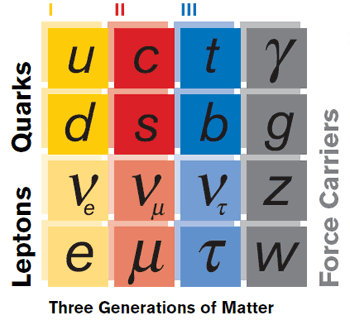
\includegraphics[width=360pt]{Figures/theory-standard-model-symmetry-mag.png}
    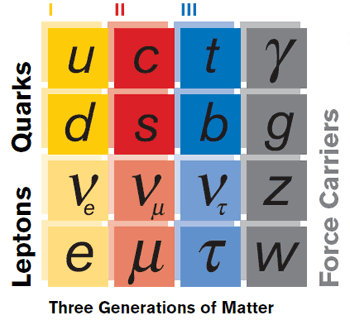
\includegraphics{Figures/theory-standard-model-symmetry-mag.png}
  \end{center}
  \caption[Particles of the standard model]
	  {Particles of the standard model that are known to exist. 
	    The Higgs boson is also predicted as part of the 
	    Standard Model, 
	    but has not yet been discovered. 

	    }
  \label{fig:StandardModel}
 \end{figure}

\section{antiparticles}
In general, each particle has an antiparticle partner, 
often denoted by a bar ($\bar{u}$), 
of the opposite charge and quantum numbers; % opposite quantum numbers in general, explain quantum numbers? because have to account for photon, gluon, Z, neutrinos
quantum numbers are used to describe the properties of the particles 
and corresponding interactions.  
For instance, all leptons have a non-zero ``lepton number;'' 
if the initial state of a set of particles 
has a total lepton number of 1, 
then any interaction between those particles will 
result in a final state with the same lepton number.  
Lepton number is always conserved in this way, 
as are charge and other quantum numbers.  
The antiparticle of the electron ($e^-$) 
has the opposite charge and lepton number 
and is called the positron ($e^+$).  
Neutrinos, being chargeless, 
have antineutrinos with opposite lepton number.  % EXPLAIN!!!!!
Quarks and gluons have another quantum ``number'' known as color.   % EXPLAIN HOW CANNOT HAVE BARE QUARKS
The three colors are red, green, and blue, with the corresponding 
``anti-colors'' being anti-red, anti-green, and anti-blue.  
%This ``color'' does not refer to our everyday experience of red, green, and blue, 
%%but there is a certain analogy to light in the ``quantum color'' behavior.  
%but the name is not accidental -- there is an analogy to colored light.  
Color is unique in that all observed states of quarks and gluons 
are ``colorless.''
In two-quark states, a color and its anti-color ``combine'' to make a colorless state.  
Three-quark states are also colorless, but through a different combination: 
the three quarks are colored red, green, and blue 
(or the corresponding anticolors), which ``combine'' (like colored light) to form 
a state with no color
In practice, antiparticles are often called by their particle names; 
since it is known that a neutral Z must decay to one positive and one negative 
particle, no distinction is made between ``positron'' and ``electron'' -- 
both are called ``electrons.''  

\section{higgs}  
Not shown in Figure~\ref{fig:StandardModel} is the Higgs boson, 
which is predicted by the Standard Model 
to give mass to the other particles.  
The Higgs has not yet been discovered; 
finding it (if it exists) is one of the 
goals of the LHC.  

\section{gravity}
The Standard Model does not include the final 
fundamental force, gravity.  
Gravity is the weakest of the forces and does not 
measurably affect interactions between fundamental particles.  
The reason that it is the only one observable on a 
cosmological scale is because its ``charge,'' mass, 
is cumulative; there is no anti-mass to counter it 
the way a negatively-charge electron and a positively-charged 
proton combine to make an electrically neutral hydrogen atom.  % put this sort of stuff in beginning?
Gravity has been described on a macroscopic scale, but 
%so far gravity has not yet been (fully?) worked into the % FIXME!!!
%framework of the fundamental particles.  
so far no theory has fully united gravity with the 
other fundamental forces.  
%There are many efforts currently ongoing to unite them, % REFERENCE?
%but none of these approaches have yet been proved.  
Such a ``theory of everything'' is 
%a dream of 
one of the goals that 
theoretical physics %.  
pursues.  

% http://www.symmetrymagazine.org/cms/?pid=1000064  the symmetry magazine SM picture
% don't know how it prints in black and white
% LATEX DOESN'T DO GIFS

TABLE OF MASSES




\section{forces and groups?}

gauge groups, little intro to group theory

A ``group'' is a set of elements with specific properties.  
In particular, any transformation of an element in the group 
results in another element in the group.  

A ``Lie'' group is one in which any transformation % NEED THIS????
can be done in very small steps, 
each of which results in an element still in the group.  
The different fundamental forces are described by different Lie groups.  

which particles feel which forces?

Each of the three forces in the Standard Model 
is described by such a Lie group.  % group. 
%In each case, the ``dimension'' of the group 
%is the dimension of the matrices
Each group is represented by a set of square matrices 
of some dimension, given by the number in parentheses.  
The matrices used for these representations are 
all unitary (hence the common ``U'' designation).  
``Unitary'' means that the matrix's inverse 
is equal to its complex conjugate transpose.  
In other words, if you flip the matrix's elements 
about its diagonal and replace each imaginary unit $i$ 
with $-i$, then multiply it by the original matrix, 
the result is the identity matrix.   % EXPLAIN IDENTITY MATRIX??

\section{EM: U(1)}
The electromagnetic force is described by the $U(1)$ group.  
Essentially, this describes rotation about an axis.  % talk about more than matrices?
The single parameter (an angle) requires only one matrix, 
corresponding to a single % force particle(s)
force carrier, the photon.  
The electromagnetic force causes interactions between 
photons and any particles that have electric charge.  
This includes quarks, leptons, and the charged weak bosons.  
%Because the photon is massless, the electromagnetic force % EXPLAIN MORE???
%can act over long distances, observable on the human scale.  

\section{Weak: SU(2)}
The weak force is represented by the $SU(2)$ group.  
The ``S'' addition in the name stands for ``special'' 
and means that each matrix's trace 
(the sum of elements along the matrix's diagonal) is zero.  
$SU(2)$ represents rotations in three dimensions 
using three matrices, 
and therefore has three parameters corresponding 
to the single angle of $U(1)$.  
These give rise to the three carriers of the weak force, 
the two oppositely-charged W's and the Z.  %%% FIGURE OUT HOW TO DO W+- in latex? sort of like writing it out longhand, but should show at least W+ and W- notation 
%All three carriers have significant mass, which means 
%the distance over which they have an effect is very small.  
The weak force acts on any particles that have the ``weak 
version'' of electrical charge, %known as %``hypercharge.''  
%``weak isospin.''
namely all fermions.  
%All fermions interact via the weak force; 
In particular, the weak force is the only way 
neutrinos interact.  
%However, interactions with W's only happen in ways  % TALK ABOUT CONSERVATION OF CHARGE IN GENERAL
%that conserve charge.  
%Hypercharge is a combination of electric charge 
%and weak isospin.  

\section{QCD: SU(3)}
Finally, the strong force is represented by $SU(3)$, 
which does not have an easy analogy to rotations 
like the previous two groups.  
It uses eight matrices, which correspond to the 
eight different gluon states that mediate the force.  
% talk about dim-3 = 3 colors?
The three dimensions of the group relate to the 
three ``color charges,'' red, green, and blue.  
Strong force interactions happen between all particles 
that carry this color charge, 
namely quarks, but also gluons themselves.  
% talk about color confinement and asymptotic freedom?  YES, but how to explain in terms of mass???
This so-called self-interaction on the part of the gluons 
causes the strong force to increase with distance.  
At short distances, the quarks making up another particle 
essentially act free; 
only when they get further apart do they feel the force 
keeping them in their bound state.  
This situation is related to the fact that quarks are 
never observed alone, only within these bound states.  
An interaction that is energetic enough to cause 
quarks to separate is also energetic enough to 
create more quarks with which the original quarks 
form new bound states.  
%When a quark gains a significant energy 
%(through an interaction with another particle), 

%This is known as color confinement
%The implication is that in spite of the fact that 
%gluons are massless, 
%the strong force is not observable over large distances.  

\section{PDFs}

Since quarks do not exist in an isolated state 
outside hadrons, 
any interaction between them must also take 
into account the structure of the protons.  
The quark structure of protons is given 
by a set of functions called 
``parton distribution functions'' or PDFs: 
\[
f_i(x)
\]
These functions represent the probability 
of finding a given quark flavor $i$ inside 
the proton with a given momentum.  
The quark's momentum itself is not used; 
rather, the fraction of the proton's 
momentum that the quark carries, or $x$. 
Since no quark can have momentum greater 
than that of the proton itself, 
the value of $x$ ranges from 0 to 1.  
%Furthermore, % do PDFs only refer to quarks??? do they necessarily integrate to 1??
A proton is said to consist of two up quarks 
and a down quark; 
however, these represent the ``valence'' quarks only.  
A ``sea'' of quarks is also present, 
formed from gluons and each existing only 
momentarily, 
illustrated in Figure~\ref{FIXME}.  
Therefore the PDFs represent all quark 
flavors, not just $u$ and $d$.  

QUARK MODEL PICTURE

PDFs cannot be calculated from first 
principles and must be measured by fits 
to experimental data.  
The currently-distributed PDF sets 
account for data from all major past experiments.  
However, there is still some uncertainty, 
%in the PDFs, 
and precision measurements of Z production 
at the LHC can %help %contribute to better PDF sets.  
improve the community's knowledge of PDFs.  

\section{ewk: SU(2)xU(1)}
The forces here have been given in terms 
of mathematical groups.  
However, the individual groups by themselves 
do not necessarily represent the reality of particles.  
It is known experimentally that the bosons carrying 
the weak force have mass.  
%The $SU(2)$ formulation of the weak force
In order for the theory to correctly predict the 
fact those particles should be massive, 
the electromagnetic and weak interactions had to be combined 
into a single framework, 
%Steven Weinberg and Abdus Salam 
%The electromagnetic and weak forces were combined into one framework, 
$SU(2) \times U(1)$, using a specific method.  
The integrated $SU(2) \times U(1)$ group 
allows for the collective four force-carrying bosons 
(photon, positively- and negatively-charged W's, and Z) 
to be described as compositions of the same underlying states.  
The elecroweak interaction has its own set of quantum 
numbers: ``weak isospin,'' and ``hypercharge,'' 
which combines weak isospin with electric charge.  
$T_3$ is the third component of the isospin 
and relates how to the fermions are arranged 
within the standard model generations 
(refer to Figure~\ref{fig:StandardModel}).  
Each generation consists of two pairs, 
one pair of quarks and one pair of leptons.  
The placement of each particle within its pair 
reflects how it interacts with the weak force.  
%This quantity is the ``weak version'' of electric charge, 
%known as ``hypercharge.''  
For the top particle in each pair, the hypercharge 
is $+\frac{1}{2}$; 
for the bottom particle, it is $-\frac{1}{2}$.  
(Note: this only applies to particles whose spin 
is ``left-handed,'' 
or oriented to spin left with respect to its direction of motion.  
Particles with ``right-handed'' spin have zero weak isospin; 
right-handed neutrinos do not interact in the Standard Model.  
This is equivalent with the assertion that neutrinos 
must be moving at the speed of light and therefore 
do not have mass. 
If neutrinos had mass, 
they would be moving slower than the speed of light 
and there could be a reference frame -- 
where the observer moves faster than the neutrino -- 
in which the neutrino would actually be left-handed.  
Because recent observations have indicated neutrinos % REFERENCE
do in fact have mass, 
this aspect of the Standard Model is inaccurate.)  

\section{spont symm break}
The fact that the three weak bosons are massive, though, 
comes from applying ``spontaneous symmetry breaking.''  
This method uses the fact that the groups mentioned 
above have underlying symmetries: 
that is, they contain parameters that do not affect the 
physical description in any way.  
They are symmetric with respect to variations in these parameters.  
However, the values of these parameters can be chosen 
in a strategic way and the result manipulated % TALK ABOUT FIELD THEORY AT ALL?? this is all lagrangians and mass terms
to give masses to the weak bosons.  
(A consequence of this ``strategic choice'' is the appearance 
of another massive particle in the theory: 
the Higgs boson.  
The Higgs boson is therefore predicted by the theoretical 
mechanism used to account for massive weak bosons.  
Time -- and collision data -- will tell if the theory 
in this form is correct.)  


\section{matrix elements/feynman rules???}

% MOVE THIS SECTION????

%Transformations within these groups can be represented as matrices.  % IS THIS ACTUALLY THE SAME AS THE GROUP MATRICES??
These matrices act on the set of initial states 
and result in the set of final states.  
Each element in the matrix, mapping a single initial state 
to a single other final state, 
gives the amplitude with which the % ONLY IN SCATTERING???  make sure this is right context 
transformation happens.  
Essentially, squaring the matrix element gives the 
relative probability of that particular transformation.  
Matrices are often used to represent transitions 
from one quantum mechanical state to another.  

This is used in particle physics as such: 
a transformation from an initial state, 
in our case two quarks from colliding protons, 
to a final state, 
an electron and a positron, 
is represented by a Feynman diagram, 
shown in Figure~\ref{fig:ZeeFeynmanDiagram}.  
The interaction can be thought to progress to the right.  
Each straight line represents a fermion, 
either the quark or the electron.  
The wavy line represents a boson, the Z.  
(Gluons are represented by curly lines.)  
The intersections between particle lines, or vertices, 
show interactions between the given particles.  
%The type of interaction can be determined by the particles   % NEED THIS?  
%taking part: 
%an interaction between a Z and a quark or lepton 
%indicates the weak force is involved.  
The matrix element corresponding to this transformation 
can be written down 
by attributing factors to the various elements 
of the Feynman diagram: 
the particle lines and the vertices.  
In this way, the diagrams are not just useful 
conceptual pictures 
but also powerful calculational tools.  
%somewhere get into spinors...

%put equation for differential cross section element 
%in terms of amplitude/matrix element 

\section{pQCD: LO, NLO, all that}

%put all qcd stuff in here?  don't need all the detail of zeus stuff

%NOT JUST QCD!  vertices in QED, too!  

However, in real life a given interaction is 
never represented by just one diagram.  
For each diagram, 
such as Figure~\ref{fig:ZeeFeynmanDiagram}, 
there is an infinite number of 
more-complicated diagrams that 
represent the same initial and final states.  
A few examples are illustrated in Figure~\ref{FIXME}.  

FIGURE WITH MORE FEYNMAN DIAGRAMS

Fortunately, the more complicated a diagram, 
the smaller its contribution.  
Each vertex in the diagram contributes 
one factor of the relevant coupling constant. % (see Section~\ref{FIXME}).  
Since the coupling constants are small, 
a two-vertex diagram contributes much more 
than a three-vertex diagram, 
which contributes more than a 
four-vertex diagram, etc.  
%The number of vertices in a diagram 
However, the corrections from the higher-vertex 
(or ``higher-order'') 
diagrams make noticeable contributions 
to the overall result, 
and therefore they should be taken into 
account as far as possible.  
Calculating the contributions from 
successively higher-order diagrams 
can be difficult, though, 
and many specialized programs exist.  
(See Chapter~\ref{sim}.)  
The simplest Feynman diagram is called 
``leading order'' (LO), 
and the successively higher levels are 
``next-to-leading order'' (NLO) and 
``next-to-next-to-leading order'' (NNLO).  
This analysis uses a theoretical 
cross section calculation that 
was done in NNLO, 
which gives a result accurate to 
around 1\%.  


\section{Electroweak Physics}
\label{theory:EWK}

lagrangian etc? i.e. more specifics on ewk physics

feynman diagrams, how they can actually be used -> 
matrix elements -> cross section element.  

\begin{figure}[htb]
\begin{center}
  \begin{tikzpicture}[
      thick,
      % Set the overall layout of the tree
%      level/.style={level distance=1.4cm, line width=0.8mm},
      level/.style={level distance=1.4cm, line width=0.5mm},
      level 2/.style={sibling distance=1.4cm},
      level 3/.style={sibling distance=1.4cm}
    ]
    \coordinate
%    child[grow=south east]{
%      child[grow=north east]{
%        edge from parent [gluon]
%        node[right]{$g$}
%      }
    child[grow=south east]{
      edge from parent [electron]
      child[grow=south west] {
        edge from parent [electron]
%        node[above] {$\bar{q}$} % ADDED
        node[below] {$\bar{q}$} % ADDED
%          child[grow=south west]{
%            edge from parent [electron]
%            node[above] {$\bar{q}$}
%          }
%          child[grow=south east]{
%            edge from parent [gluon]
%            node[right] {$g$}
%          }
      }
      child[grow=east, level distance=2.4cm] {
        child[]{ % added the [], did nothing, don't know how to make angle of line the same as LHS
          edge from parent [electron]
          node[below] {$e^{-}$}
        }
        child[]{ % added the [], did nothing, don't know how to make angle of line the same as LHS
          edge from parent [electron]
          node[above] {$e^{+}$}
        }
%        edge from parent [boson]
        edge from parent [zboson]
%        node[below] {$Z/\gamma*$}
        node[below] {$Z$}
      }
%    }
      edge from parent [electron] node [above=3pt] {$q$}
    };
  \end{tikzpicture}
\end{center}
%  \caption[Feynman diagram of \qqZgee]
  \caption[Feynman diagram of \qqZee]
%	  {Feynman diagram of \qqZgee.  
	  {Feynman diagram of \qqZee.  
	    }
  \label{fig:ZeeFeynmanDiagram}
\end{figure}

where to put cross section formula stuff 
-- make new section?
(and which stuff to use?)

order of diagram = number of vertices!  

\subsection{Z Production}
\label{theory:Zprod}

someplace need to go into 4-momenta...

s, inv mass, pdfs attach to tree-level matrix element, 
Z/gamma* interference

s = Z mass -- well, dunno, also includes momentum

\section{relativistic kinematics}

A particle's coordinates can be described in terms of 
four quantities: its three spatial coordinates 
and its point in time.  This is conventionally 
represented as 
\[
x^{\mu} = (t, x, y, z)
\]
(where we are treating the speed of light to be 
equal to 1).  
Moving at relativistic speeds, 
or being viewed from a relativistic reference frame, 
can change the relation between these 
four quantities at any point.  
However, a certain combination is 
invariant -- that is, it remains the same no 
matter the speed or reference frame.  
This invariant can be constructed as 
\[
t^2 - x^2 - y^2 - z^2 = x^{\mu} x_{\mu}
\]

In the same way, a particle's motion can be described 
in terms of its energy and the three components of 
its momentum, called ``four-momentum:''
\[
p^{\mu} = (E, p_x, p_y, p_z)
\]
The invariant combination is called ``invariant mass'' 
and is equal to the particle's rest mass.  


PUT INV MASS UP HERE

\section{kinematics like s}
The quantity $s$ is the square of the center-of-momentum 
energy of the colliding proton system.  
(Therefore $\sqrt{s}$ is the center-of-momentum 
energy itself.)  
It is obtained by adding together the four-momenta 
of the colliding protons, designated $1$ and $2$: %.  
\[
s = (p_1 + p_2)^2
\]
However, since only a single quark participates 
in the interaction, not the full proton, 
the energy of the interaction must be reduced.  
Since $x$ the fraction of the proton's momentum that is carried 
by the quark (see Section~\ref{FIXME}), %is defined $x$, so that 
the 
quark's momentum is then $xp$.  
We can then define a center-of-momentum energy, 
$\hat{s}$ (or $Q^2$), 
for the quark-quark system, 
the interacting part of the proton system: 
\[
\hat{s} = (x_1 p_1 + x_2 p_2)^2
\]
This can be approximated in terms of the original 
(proton) $s$ as 
\[
\hat{s} \simeq x_1 x_2 s
\]




\section{calculating xsec FORMULAS}

%!!!! THIS IS ALL FOR PHOTONS DRELL YAN !!!!!
%is that okay?????????
%Z's have different feynman rule factors!!


%more specific derivation stuff?  
%I guess, if I'm starting from the 
%feynman diagram stuff

The concept of the cross section was introduced previously, 
in terms of how to calculate it from experimentally-measured 
quantities.  
%Knowing the underlying physics, though, 
%the cross section can be calculated 
In principle, though, the cross section 
can also be calculated from the underlying physics.  
%The cross section can be expressed as 
%\[
%Cross section = \frac{W_{fi} }{\mathrm{initial flux}}
%\times (\mathrm{number of final states})
%\]
%$W_{fi}$ is the rate of transition from the initial state 
%to a given final state, expressed per unit volume.  
%The greater the number of possible final states, 
%the more likely a transition is to occur.  
The cross section element for a transition 
between two states can be expressed as 
% the VERY beginning of the cross section formula
% where |M|2 is ``probability'', F is flux = particles per area per time, 
% and dQ is dLIPS
\[
d \sigma = \frac{ \left| \mathcal{M} \right| ^2 }{F} d Q
\]
In this formula, $\mathcal{M}$ is the amplitude 
(or matrix element) governing the probability of 
transitioning from the initial state to the final state, 
$F$ is the particle flux, and $d Q$ is the 
phase space element.  
An initial state within the phase space element $d Q$ will 
contribute the element $d \sigma$ to the overall 
interaction cross section.  
Therefore, to get the full cross section, one must integrate 
over the full phase space.  
%Doing this in the center-of-momentum frame results 
%in the formula for the differential cross section 
For an interaction with two initial particles and 
two final particles 
(a $2 \rightarrow 2$ interaction), 
this can be integrated partially to 
% (in CM) the full differential cross section is 
% for any given feynman diagram
\[
\frac{d \sigma}{d \Omega} \bigg| _{CM} 
= \frac{1}{64 \pi^2 s} \frac{p_f}{p_i} \left| \mathcal{M} \right| ^2
\]
where $p_i$ and $p_f$ are the momenta of the initial and final particles 
(in the center-of-momentum frame with two particles, 
the initial and final momenta each have the same magnitude).  
Here $d \Omega$ is the solid angle element; 
the formula cannot be further integrated without knowing the 
(angular-dependent) form of $ \left| \mathcal{M} \right| ^2 $.  
% where d\Omega is solid angle element
% pf and pi are the initial and final momenta of each element,
% since in CM pi1 = pi2, pf1 = pf2
% differential is eventually integrated

%% % now for curly M squared
%% % Feynman diagram sez 
%% \[
%% \mathcal{M} = -
%% \]

%curly M can be written down from Feynman rules, 
%according to tensor structure

For any given Feynman diagram, 
such as Figure~\ref{fig:ZeeFeynmanDiagram}, 
a set of rules makes it possible to write 
down the elements of the interaction amplitude, 
$\left| \mathcal{M} \right| ^2$.  
%Due to the nature of electroweak interactions 
Electromagnetic interactions are fairly 
simple in structure and can be written down 
(and then calculated out) relatively easily.  
Electroweak interactions are somewhat 
more complicated.  
The full differential cross section for the interaction 
%the giant thing from the PDG RPP CH 40:
%while the giant thing is given by 
%(full differential cross section for 
%$ f_i \bar{f_j} \rightarrow (W,Z) \rightarrow f_{i'} \bar{f_{j'}} $
$ q_A \bar{q_B} \rightarrow Z \rightarrow e_{C} \bar{e_{D}} $
(where $q_A$ and $\bar{q_B}$ are the initial quarks 
and $e_{C}$ and $\bar{e_{D}}$ are the final electrons) is given by 
%\[
%\frac{d \sigma}{d \Omega} = \frac{N_c^f}{N_c^i} 
%\times \frac{1}{256 \pi s} 
%\times \frac{s^2}{(s - m_Z^2)^2 + s \Gamma^2}
%\times \left[(L^2 + R^2) (L'^2 + R'^2) (1 + \cos^2 \theta)
%+ (L^2 - R^2) (L'^2 - R'^2) 2 \cos \theta \right]
%\]
%Initial particles are quarks: 
%\[
%N_c^i = 3
%\]
%Final particles are leptons: 
%\[
%N_c^f = 1
%\]
\[
%\frac{d \sigma}{d \Omega} (\qqZee) = \frac{1}{3} 
\frac{d \sigma}{d \Omega} 
( q \bar{q} \rightarrow Z \rightarrow e^+ e^- ) 
= \frac{1}{3} 
\times \frac{1}{256 \pi s} 
\times \frac{s^2}{(s - m_Z^2)^2 + s \Gamma^2}
\times \left[(L^2 + R^2) (L'^2 + R'^2) (1 + \cos^2 \theta)
+ (L^2 - R^2) (L'^2 - R'^2) 2 \cos \theta \right]
\]
$\Gamma$ is the \Zee decay's 
partial width (see Section~\ref{FIXME}) 
given by 
%% \[
%% \Gamma(Z \rightarrow f \bar{f} )
%% = N_c \frac{ \sqrt{2} G_F m_Z^3 }{6 \pi}
%% \times \left[(T_3 - Q_f \sin^2 \theta_W )^2 
%% + (Q_f \sin \theta_W )^2 \right]
%% \]
\[
\Gamma (Z \rightarrow e \bar{e} )
= \frac{ \sqrt{2} G_F m_Z^3 }{6 \pi}
\times \left[(T_3 - Q_f \sin^2 \theta_W )^2 
+ (Q_f \sin \theta_W )^2 \right]
\]
The $L$ and $R$ in the cross section equation 
refer to factors from %relating to the 
left-handed and right-handed initial quarks, respectively 
(likewise $L'$ and $R'$ refer to the final electrons).  
These factors are 
%For Z, couplings are 
\[
L = \sqrt{ \frac{8 G_F m_Z^2}{\sqrt{2} } }(T_3 - \sin^2 \theta_W Q)
%L = g (T_3 - \sin^2 \theta_W Q)
\]
\[
R = - \sqrt{ \frac{8 G_F m_Z^2}{\sqrt{2} } } \sin^2 \theta_W Q
%R = - g \sin^2 \theta_W Q
\]
%``$T_3$ is weak isospin of initial left-handed fermion and 
%Q is initial fermion's electric charge. [FRACTIONAL] 
%The expressions for L' and R' are analogous.  
%The color factors $ N_c^{i,f} $ are 3 for initial or final quarks 
%and 1 for initial or final leptons.''  
$T_3$ is the weak isospin of the left-handed particle 
(the right-handed particle has isospin 0, 
hence $T_3$ does not show up in $R$). 
$Q$ is the particle's electric charge.  
%BUT, initial particles are all flavors of quarks, 
%so can't just plug in flavor-dependent quantities 
%like $T_3$ and $Q$.  
%MUST SUM OVER FLAVORS.  oh boy!
The $T_3$ and $Q$ values for the relevant particles are 
given in Table~\ref{FIXME}.  

TABLE

Since the final-state particles are already known to be electrons, 
their values can be plugged into the equation.  
However, the flavor of the initial quarks is not known.  
Therefore, all the possible initial quark states must 
be taken into account, by adding up the contribution from each one.  

%H+M have SUCH a nice little summary in the inside back cover.  

%can put in terms of little g:
%\[
%g = \sqrt{ \frac{8 G_F m_Z^2}{\sqrt{2}} }
%\]


%% % WHICH simplifies to give us AVGD OVER SPINS or whatever
%% \[
%% \bar{ \left| \mathcal{M} \right| ^2 } 
%% = 2 e^4 \left[ \frac{1}{2} \left( 1 + \cos^2 \theta \right) \right]
%% \]

%% % THEN
%% \[
%% \frac{d \sigma}{d \Omega} \big| _{CM}
%% %= \frac{\alpha^2}{4s} \left( 1 + \cos^2 \theta \right) 
%% = \frac{\alpha^2}{4 Q^2} \left( 1 + \cos^2 \theta \right) 
%% \]


% quark-level subprocess is 3 e_q^2 times that for muons
% DON'T NEED TO SHOW THIS, backwards anyhow
%\[
%\sigma(e^- e^+ \rightarrow q \bar{q} ) 
%= 3 e_q^2 \sigma(e^- e^+ \rightarrow \mu^- \mu^+ )
%\]

%% % WHERE
%% %\[
%% %\sigma(e^- e^+ \rightarrow \mu^- \mu^+ ) 
%% %= \frac{4 \pi \alpha^2}{3 s}
%% %\]
%% % don't need to show that one either, 
%% %just result: 
%% \[
%% \sigma ( q \bar{q} \rightarrow e^- e^+ )
%% %= 3 e_q^2 \frac{4 \pi \alpha^2}{3 s}
%% = 3 e_q^2 \frac{4 \pi \alpha^2}{3 Q^2}
%% \]
%% % D'OH, look at next line!

%% % cross section of quark-level subprocess
%% \[
%% \hat{\sigma} (q \bar{q} \rightarrow l^- l^+) 
%% = \frac{4 \pi \alpha^2}{3 Q^2} e_q^2
%% \]

% but need to account for the proton and pdfs

%In addition, 
However, the interaction does not happen 
between two quarks in isolation.  
The cross section calculation must take 
into account the fact that the quarks come from 
protons with internal structure.  
The following formula gives the full cross section 
in terms of the one given by the quark-level diagram: 
%% \[
%% \frac{d \sigma}{d Q^2}(pp \rightarrow f \bar{f} )
%% = \left( \frac{1}{3} \right) \left( \frac{1}{3} \right) 3 
%% \sum_q \int dx_1 \int dx_2 f_q (x_1) f_{\bar{q}} (x_2)
%% \frac{d \hat{\sigma} }{d Q^2}
%% \]
\[
\frac{d \sigma}{d Q^2}(pp \rightarrow e^+ e^- )
= \left( \frac{1}{3} \right) \left( \frac{1}{3} \right) 3 
\sum_q \int dx_1 \int dx_2 f_q (x_1) f_{\bar{q}} (x_2)
%\frac{d \hat{\sigma} }{d Q^2}
%\frac{d \sigma }{d Q^2}(\qqZee)
\frac{d \sigma }{d Q^2}
( q \bar{q} \rightarrow Z \rightarrow e^+ e^- )
\]
Here $q$ is the sum over the possible quark flavors 
and $f_q(x)$ are the parton distribution functions 
(see Section~\ref{FIXME}) for each quark flavor.  
Since the Z differential cross section depends 
on the PDFs in this way, 
it is useful as a test of current PDF knowledge.  
Precision measurements of the differential cross section 
can distinguish between different implementations 
of the PDFs.  

%% % ... which gives
%% % THE BIG FAT GIANT CROSS SECTION EQUATION 
%% % in terms of the parton distribution functions f_i(x)
%% \[
%% \frac{d \sigma}{d Q^2}(pp \rightarrow l \bar{l} X)
%% = \frac{4 \pi \alpha^2}{9 Q^4} 
%% \sum_q e_q^2 \int dx_1 \int dx_2 f_q (x_1) f_{\bar{q}} (x_2) 
%% \delta \left( 1 - x_1 x_2 \frac{s}{Q^2} \right)
%% \]

%do I have to go all the way through the cross section stuff???  yeah, I think so...

%THIS IS ONLY LOWEST ORDER, with no ISR/FSR gluon emission stuff. 
%TALK ABOUT CORRECTIONS!!!!!

However, this formula only gives the cross section 
for the simplest Feynman diagrams; 
higher-order diagrams contribute as well.  
As mentioned previously, various programs 
in existence attempt to include some of these higher-order 
diagrams in their calculations.  


\section{inv mass}
%The definition of a 
A particle system's ``invariant mass'' is 
a combination of its energies and momenta that 
remain unchanged regardless of reference frame.  
A particle (or everyday object) can appear to 
have a different energy depending on the reference 
frame from which it is viewed.  
If you are sitting on an airplace at cruising altitude, 
the plane is not moving with respect to your body.  
However, if you are on the ground, the plane is 
moving very fast -- 
it has a different kinetic energy in that frame.  
The physics of the situation cannot depend on 
the reference frame of the observer, 
even at the relativistic speeds of interacting particles.  
The invariant mass is such a quantity that 
remains the same.  
In addition, since the energy and momentum 
of a system are conserved, 
the invariant mass is also conserved 
throughout the entire interaction, 
in particular the decay.  
The general definition is given as 
\[
M_{inv}^2 = \left( \sum E \right)^2 - \left\| \sum \mathbf{p} \right\|^2
\]
For a single particle, the expression simplifies 
to the particle's mass.  
This analysis makes use of the fact that the 
invariant mass of the decay particles 
(the two electrons) 
is the same as the (invariant) mass of the 
particle which decayed, the Z.  
The above formula, simplified to two particles, 
\[
M_{inv} = \sqrt{ \left(E_1 + E_2\right)^2 - \left\|\mathbf{p}_1 + \mathbf{p}_2\right\|^2 }
\]
reconstructs the mass of the Z boson 
based on the energies and momenta 
of the decay products.  
%The Z's $M_{inv}^2$ is also the energy 
%of the interaction, $\hat{s}$ 
%(see Section~FIXME).  


\section{dy interference}
Another diagram contributes to the process being studied. 
In this case, a photon replaces the Z boson 
as the link between the quarks and the electrons.  
Because these diagrams have the exact same 
initial and final states, 
they ``interfere'' with each other.  
Experimentally, it is impossible to tell which one happened; 
both must be included in the calculations.  % is this exactly why???

BOTH DIAGRAMS SIDE-BY-SIDE

It is necessary to note that the photon that takes 
part in this interaction is a ``virtual'' photon -- 
%it cannot be observed by itself.  
it cannot be directly observed.  
The reason for this is that there is always a 
center-of-momentum reference 
frame for the two particles colliding to form the photon.  
In other words, there is always some way that you, 
the observer, can be moving, 
such that it looks like the two particles 
have the same speed but opposite directions.  
In this reference frame, the photon would be formed at rest, 
which violates the principle that the speed of light 
is the same in all reference frames -- 
the speed of light can never be zero.  
Equivalently, such a photon would have mass, 
while real photons are massless.  
The mass of this virtual photon is indeed the same 
as the invariant mass of the system.  
%Such virtual particles can exist due to inherent   %% is that actually why these photons in particular can be virtual?  
%fluctuations in energy, by the uncertainty 
%principle of quantum mechanics.  
Such virtual particles are allowed to exist 
by the uncertainty principle of quantum mechanics, 
which governs the ``borrowing'' of energy from the vacuum.  
The smaller the time scale over which the energy 
fluctuation happens, 
the larger the energy fluctuation allowed.  
\section{off-shell}
Having a specific mass defines a thin 
surface or ``shell'' in kinematic phase space; 
only certain combinations of energy and momentum 
are allowed, 
because of the relations between mass, energy, and momentum.  
Particles that are virtual, 
i.e. have a mass much different than their 
defined ``real'' mass, 
are called ``off-shell'' -- 
they are ``off the mass shell.''  
\section{Z can be offshell like photon, that's why it's a distribution with a peak with a width}
The Z boson, while it has a defined mass, 
%DECAY WIDTH ETC ETC ETC 
can be ``off-shell'' in the same way as the photon.  
That is, in general the 
%reconstructed 
mass 
does not take on a single precise value; 
instead, over many events it manifests as a distribution 
peaked around the ``real'' value.  
This is typical of particles that are measured only 
by their decays, called ``resonances;'' 
these particles tend to be at least slightly virtual 
%because they are not being observed directly.  
because of their short lifetimes.  
%in fact, 
\section{decay lifetime partial width}
In addition, the width of the peak is inversely prorportion to the   % how relevant is this actually?  in cross section formula
lifetime of the particle.  
The wider the peak, the more final states the particle can decay into, 
and the more likely it is to decay.  
The contribution of each final state is called the 
``partial width;'' 
this quantity plays a role in calculating 
how often a given resonance is produced.  

PIC OF DY SPECTRUM??

%PUT DY CROSS SECTION FORMULA STUFF HERE, 
%saying it's simpler in form.  
%ALSO NEED TO EMPHASIZE CROSS SECTION NOT ADDITIVE.  
%matrix elements interfere.  

The cross section for the photon process 
is more easily calculated and is given by the formula
\[
\sigma(q \bar{q} \rightarrow e^+ e^-) 
= \frac{4 \pi \alpha^2}{3 Q^2} e_q^2
\]
However, the cross sections of the Z and the photon 
processes are not additive; 
rather, the diagrams interfere, 
so the full amplitude must be calculated taking 
both into account at once.  

In this case, only the area around the Z peak is being 
studied, not the full spectrum.  
The main contribution in this area is the Z itself; 
%as opposed to virtual photons.  
however, the photon contribution must still be included 
in the discussion.  


\subsubsection{Results from Previous Experiments}
\label{theory:prev}

\subsection{Z Decay}
\label{theory:Zdec}
need this section??


somewhere have intro to QFT and all that?  

also, explanatory items from overview:

   * [here or] in theory chapter define ``tree-level''.  
ALSO IN THEORY: explain how Feynman diagrams are so useful! 
writing down the matrix element and all that
AND PDFs, basically whole process of stuff simulated 
really happens and should be explained.  
AND DEF OF PARTONS
yeah, basically explain all the stuff in the MC chapter
INCLUDING ISR and FSR
ALSO define ``jets'' and talk about how they come from 
quarks and gluons (define partons) and relate to ``hadronization'' -- 
not entirely relevant for this analysis, 
but possible in general
AND define ``color''
AND asymptotic freedom, how it takes more and more energy to get them further apart

   * intial- and final-state radiation

%   * [HERE OR IN THEORY INTRO] need to do on-shell/off-shell decays 
%to explain why Z mass has a spectrum and not a single value

%   * invariant mass (here?)

   * cross section formula and matrix elements and what said matrices do

   * PDFs, what they are, how they relate to Z physics

AND, of course read the others' theses to see what they had in here, too.  




\chapter{Experimental Setup}
\label{exp}

\section{CERN}
\label{exp:CERN}
The European Organization for Nuclear Research, or CERN, is an
international laboratory just outside Geneva, Switzerland.  
It was founded in 1954 as a collaborative effort between twelve European 
countries.  
It now has twenty member states, as well as many observer 
and other non-member states, and is one of the world's major 
particle physics facilities.  
%Europe, founded 1959?, maybe little significant history.  

\section{Large Hadron Collider}
\label{exp:LHC}
%All the good stats on the LHC: circumference, (place,) dipole design, magnets, magnetic field.  
%Design energy and luminosity.  how beam is actually accelerated.  
%And pictures!  diagram of LHC, diagram of magnets?  just going through prelim diagrams here!
%maybe done need one of magnets

%Accelerator chain? LINAC2->PS boosters->PS->SPS->LHC
% http://public.web.cern.ch/public/en/Research/AccelComplex-en.html

% iCMS on Nov. 20, 2010
% Maximum luminosity = 204.78 1030 cm-2s-1
% Recorded luminosity = 43.17 pb-1

The Large Hadron Collider (LHC) \cite{LhcMachine}
is a circular particle accelerator near Geneva, Switzerland, 
with a circumference of 27 km. 
Two proton beams circulate in opposite directions around the ring
and cross at several points, which are home to large particle detectors.  
Figure \ref{fig:LHCDiagram} shows a diagram of the LHC layout.  
The two general-purpose detectors, CMS and ATLAS, sit on opposites sides of the ring, 
while the two smaller specialty detectors, LHCb and ALICE, 
sit at the interaction points to either side of ATLAS.  
Each beam consists of a series of proton bunches, 
with a maximum of 2835 ``buckets'' in the beam to be filled by bunches.  
The bunch structure is such that the nominal bunch crossing rate is 40 MHz.  

The proton beams are accelerated from injection energy by %a 
radio frequency (RF) cavities, %chamber, % Wesley
which provides an energy boost with each circulation of the beam
until the collision energy is achieved.  
The beams are steered around the ring by 8-Tesla magnetic fields produced in 
15-meter-long superconducting niobium-titanium dipole magnets,
and focused by quadrupole magnets, 5-7 m long.  
The LHC uses a design in which both proton beampipes are contained in the same housing,
allowing the same liquid helium cooling system to serve both.  

The LHC began colliding proton beams in March 2010, 
quickly reaching its 2010 center-of-mass operating energy of 7 TeV
(3.5 TeV per proton beam).  
At this energy it delivered over 47 pb$^{-1}$ of collisions, 
with a maximum instantaneous luminosity of over 2*10$^{32}$ cm$^{-2}$s$^{-1}$.  
The LHC maximum design energy is 14 TeV (7 TeV per beam), 
and its design luminosity is 10$^{34}$ cm$^{-2}$s$^{-1}$.  

 \begin{figure}[htb]
  \begin{center}
    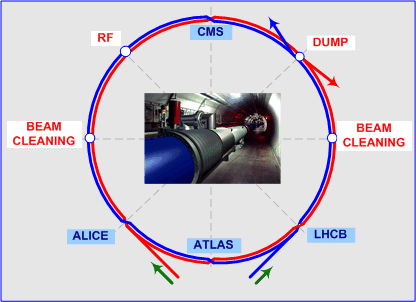
\includegraphics[width=360pt]{Figures/lhc-schematic-ml.png} 
  \end{center}
  \caption[\fixspacing Diagram of the LHC layout]
	  {\fixspacing Diagram of the LHC layout.}
  \label{fig:LHCDiagram}
 \end{figure}


\section{Compact Muon Solenoid}
\label{exp:CMS}
%SUBDETECTORS: material, coverage, resolution (spatial and energy/mom/whatever)

%Important stats on CMS: height, weight, etc.  diagram of detector.  
%Current status on detector, data-taking, event display -- here? or after everything explained?  
%At collision energy (7 TeV), CMS recorded 35 pb-1 of good data (but 43 recorded sez lumi plot)

The Compact Muon Solenoid (CMS) \cite{CmsExperimentAtCernLHC}
is one of the two general-purpose experiments for the LHC.  
Figures \ref{fig:CMSDiagram3D} and \ref{fig:CMSDiagramFlat} 
show the structure of the CMS detector.  
It is cylindrical, 21.5 m long and with a 15-m diameter, and weighs 12,500 tons.  
The overall structure of the detector is formed by the iron yoke framework surrounding the inner detector,
with the central section, the ``barrel'', divided into five ring-shaped slices, 
while each end of the cylinder, or ``endcap'', consists of several circular plates.  
These sections fit around the solenoid and inner detector, enclosing it completely.  

Particle detection is done by several dedicated subdetectors.  
The electromagnetic and hadronic calorimeters fit inside the solenoid, 
with the tracking system inside the calorimeters.  
The three components of the muon system are outside the solenoid,
integrated with the iron magnetic field return yoke:
the drift tube chambers, resistive plate chambers,
and cathode strip chambers.  

%Figure: CMS diagram, Fig. \ref{fig:CMSDiagram}
% also nice one in HLT paper

 \begin{figure}[htb]
  \begin{center}
    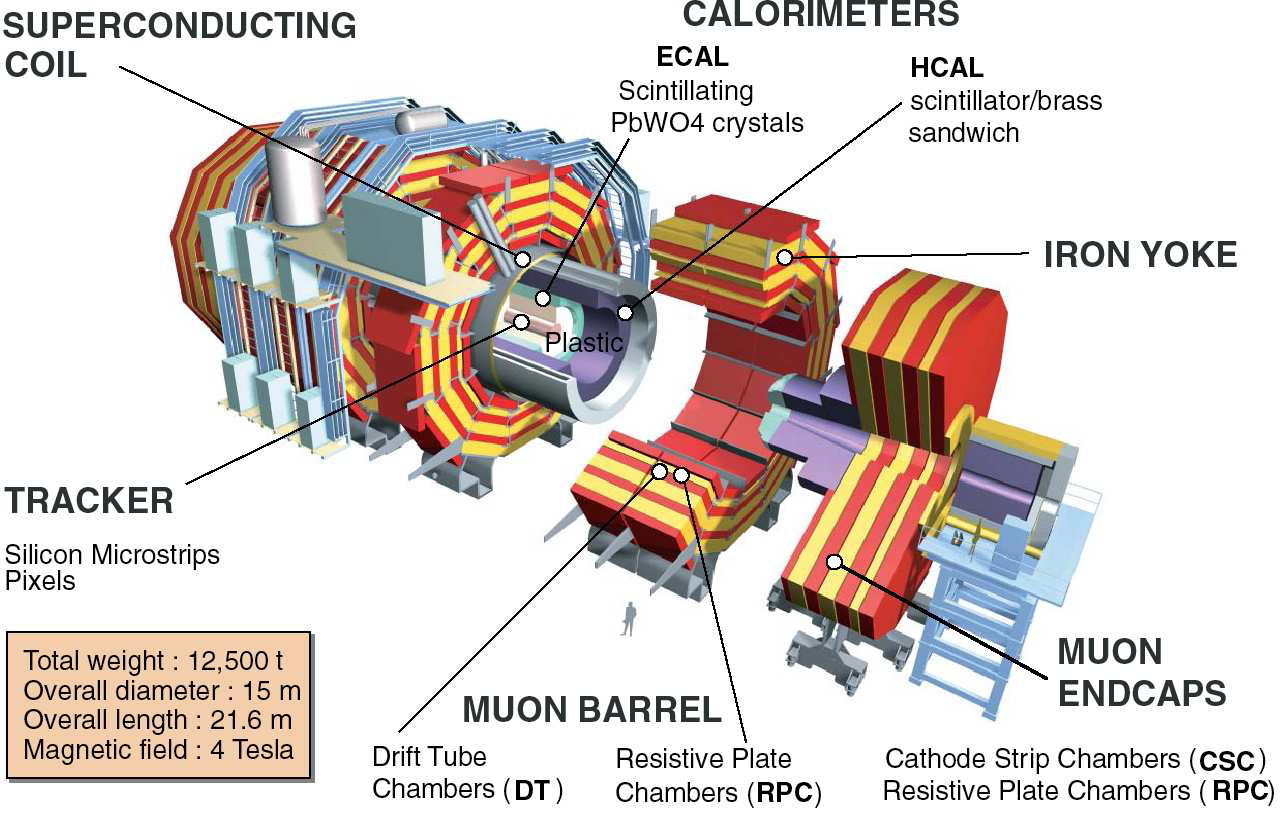
\includegraphics[width=360pt]{Figures/CMSncLabels.png}
  \end{center}
  \caption[\fixspacing Expanded view of the CMS detector]
	  {\fixspacing Expanded view of the CMS detector, showing the ring and slice structure as well as the placement of each subsystem.}
  \label{fig:CMSDiagram3D}
 \end{figure}

 \begin{figure}[htb]
  \begin{center}
    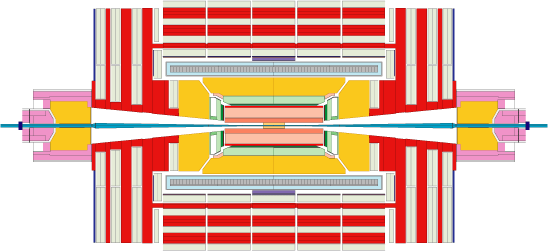
\includegraphics[width=360pt]{Figures/Longnc.png}
  \end{center}
  \caption[\fixspacing Cross-sectional view of the CMS detector]
	  {\fixspacing Cross-sectional view of the CMS detector.}
  \label{fig:CMSDiagramFlat}
 \end{figure}

\subsection{Detection of Particle Interactions}
\label{exp:particleDetection}
%Figure: Particle detection in CMS, Fig. \ref{fig:CMSParticles}

 \begin{figure}[htb]
  \begin{center}
    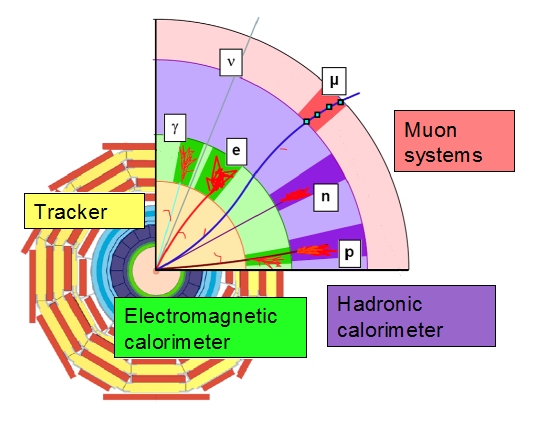
\includegraphics[width=360pt]{Figures/CMSParticles.png}
  \end{center}
  \caption[\fixspacing Detection of particles in the CMS detector]
	  {\fixspacing Detection of particles in the CMS detector.}
  \label{fig:CMSParticles}
 \end{figure}

The various parts of the CMS detector work together to differentiate
the final particles produced in proton interactions.  
As 
%the end-product 
these % I think; Wesley
particles traverse their outward trajectory,
they pass through the different subdetectors in turn.
Figure \ref{fig:CMSParticles} shows how 
%end-product 
final % Wesley
particles 
interact with the subsystems of the CMS detector.  
The innermost subdetector is the tracker, 
which reconstructs a particle's track through it
from a set of points where it detected an interaction.  
The tracker only registers particles with an electric charge; %, 
%such as electrons or muons;
neutral particles pass through undetected.  
The electromagnetic calorimeter detects particles that interact
primarily electromagnetically. %, 
%such as electrons and photons.
%Since pions, which are hadrons, can interact in the ECAL like eg particles, 
%have ES in endcap BUT PUT THIS IN ECAL SECTION
In this way the first two ``layers'' of the detector can differentiate
electrons from photons: 
both are seen in the electromagnetic calorimeter, 
but only electrons leave traces in the tracker.
Outside of the electromagnetic calorimeter is the hadronic calorimeter,
which primarily detects hadrons.  
Hadrons are also detected in the electromagnetic calorimeter,
but they leave the largest signature in the hadronic calorimeter,
which differentiates the hadrons from the electromagnetic particles
like electrons and photons.  
Hadrons are often found in large quantities called ``jets'' 
(see Section~\ref{theory:HigherOrderDiagrams}),
so summing together the energy deposits from sizable electromagnetic 
and hadronic calorimeter regions is important in event reconstruction.  
Surrounding the tracker and the calorimeters is the solenoid,
which generates the magnetic field.
The charge of a particle can be determined from which way it
bends in the magnetic field.
Finally, outside the solenoid and interwoven with the panels of the 
iron return yoke, is the muon system.  
Muons leave traces in the inner subdetectors, 
but they are the only particles to live long enough to reach the
muon system.
This differentiates them from the other particles detected by 
the inner subdetectors.  
Since the muon system is outside the solenoid, 
the magnetic field points in the opposite direction,
and hence the muon trajectories bend in the other direction
from what they had inside the solenoid.  
The last category of end-product, neutrinos, 
generally cannot be detected.
However, their direction and energy in the radial plane 
can be reconstructed 
by summing the energy of all the particles in the event.
Because the initial protons have zero momentum in the radial plane, 
and momentum is always conserved, 
any significant ``missing'' component to the final energy
can be taken to be due to a neutrino.  

A CMS event display from 2010 running can be seen in Fig. \ref{fig:EventDisplay}.  

 \begin{figure}[htb]
  \begin{center}
    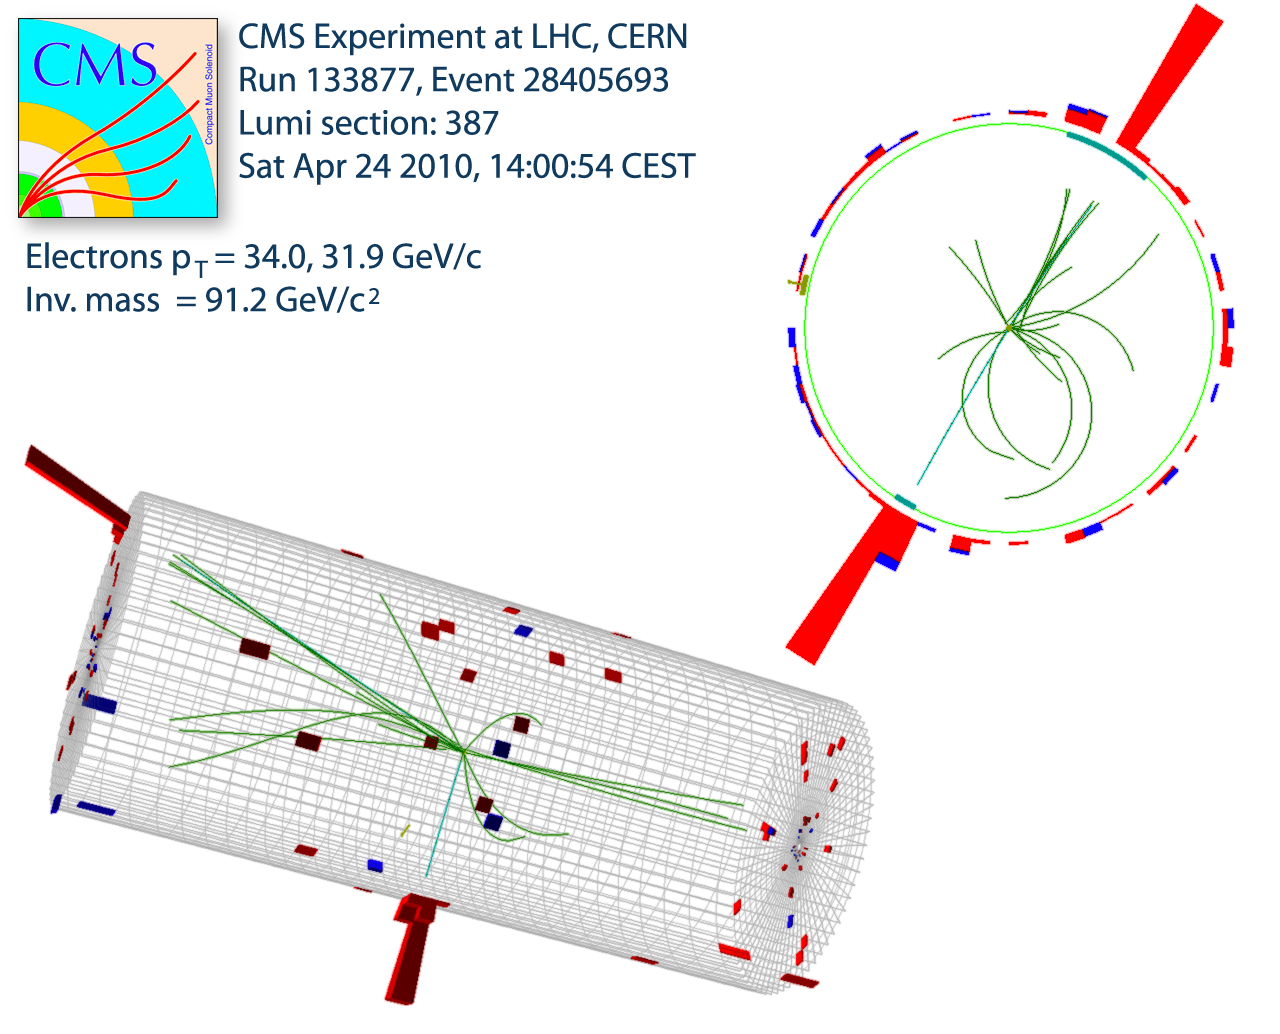
\includegraphics[width=360pt]{Figures/zee-133877-28405693-full.png}
  \end{center}
  \caption[\fixspacing Three-dimensional display of a \Zee event in the CMS detector]
	  {\fixspacing Three-dimensional display of a \Zee event in the CMS detector.}
  \label{fig:EventDisplay}
 \end{figure}

\subsection{Coordinate System} %define eta and phi earlier? YES
\label{exp:coords}
A standardized set of coordinates is used to describe points and directions within the CMS detector.  
The origin of the coordinate system is at the interaction point,
with the $x$-direction pointing horizontally south towards the LHC center
(ignoring the slight tilt of the LHC ring with respect to the vertical),
and the $y$-direction pointing directly upwards.  
The $z$-axis points horizontally west along the beam direction,
and the magnetic field inside the solenoid points in the positive $z$-direction.  
The azimuthal angle $\phi$, measured in the $x$-$y$ plane and ranging from $-\pi$ to $+\pi$ radians, 
is oriented such that $ \phi = 0 $ is equivalent to the positive $x$-axis
and $ \phi = \pi/2 $ is equivalent to the positive $y$-axis.  
The longitudinal angle $\theta$ is measured from the positive $z$-axis, 
and the sign of $ \eta = -\ln\tan(\theta/2)$ is equal to the sign of $z$.  

\subsection{Magnet}
\label{exp:magnet}
%Stats about the magnet!  how much field, how much current, weight, what it's made of,
%what makes it special

Since charged particles bend in a magnetic field, 
particle detectors use some sort of magnetic field to determine 
the charges of decay products.  
CMS uses a solenoid, or electromagnet in the shape of a coil, 
to produce a uniform magnetic field in the detector's inner region.  
The magnet coil is 12.5 m long with a 6 m diameter, 
and it weighs 220 metric tons.  
The CMS solenoid is made of a superconducting material, 
a niobium-titanium alloy, 
to handle the large amount of current necessary: 
it generates a field of 4 Tesla using 
a current of almost 20 kA in a four-layer winding.

The magnetic field is returned through a 10,000 metric ton iron yoke, 
which also serves as a support structure for the detector.  
The yoke consists of three concentric cylinders divided into the same 
5-ring barrel and 3-disk endcap structure as mentioned previously.  

\subsection{Tracker}
\label{exp:tracker}
The purpose of the tracker is to detect the 
tracks from end-product particles;
only those which are charged can be detected in the tracker.  
The CMS tracker contains 75 million channels
and is specifically designed to get good performance 
using only a small number of hits per track.
%very fine accuracy (10 um) in order to reconstruct vertices and decays (?)
It is the innermost layer of the CMS detector
and is made up of two different systems: 
the pixel detector, 
which is closest to the interaction point and hence has the finer granularity, 
and the strip tracker, 
covering the volume out to the calorimeter. 
Both systems are made of silicon and register charged particles in the same way. 
When a charged particle passes through the silicon,
it knocks electrons out of the material, 
creating a net positive charge.  
The electric current needed to return the silicon
to its neutral state is measured and amplified
by the readout electronics.  
This readout technology is fast compared to the 
25 ns bunch spacing of the LHC.  
A single track is reconstructed by stringing together
the measurements from each of the layers.  

\subsubsection{Pixels}
\label{exp:pixels}
The silicon pixel detector 
%has 
requires % Wesley
a very fine accuracy
due to the high density of tracks near the interaction point.  
It consists of 65 million readout channels 
arranged on modules in several layers around the interaction point.
In the barrel, the layers are cylindrical and situated at
radii of 4, 7, and 11 cm, 
while each endcap has two disks, at 6 and 15 cm from the
interaction point. 
Each module consists of a rectangular array of 100 $\mu$m x 150 $\mu$m pixels, 
with a resolution of \~15 $\mu$m.  
The pixels on each module are read out by a dedicated chip attached 
to the module. 
The chip contains readout unit cells, one corresponding to each pixel,
which are connected to the pixels with a small bump of solder 
in the so-called bump-bonding method.  

 \begin{figure}[htb]
  \begin{center}
    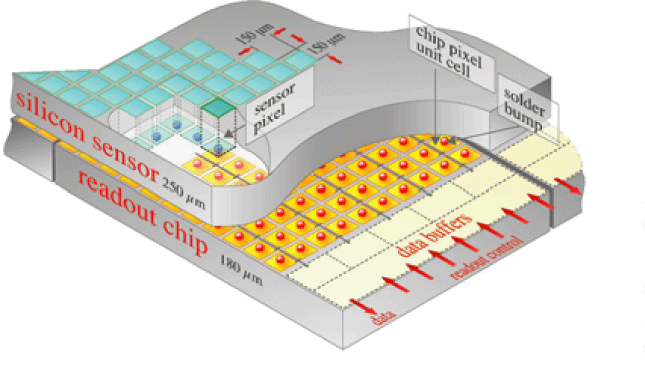
\includegraphics[width=360pt]{Figures/tracker-Pixelement.png}
  \end{center}
  \caption[\fixspacing Structure of pixel detector layers]
	  {\fixspacing Structure of pixel detector layers.}
  \label{fig:PixelLayers}
 \end{figure}

\subsubsection{Strips}
\label{exp:strips}
The silicon strip detector consists of 10 million channels
arranged in 10 layers of strips, 
in both the barrel and the endcap,
and extends to a radius of 130 cm from the interaction point
and to an $|\eta|$ value of 2.5.  
The track density at this stage is much less than in the pixel detector,
so the granularity does not need to be as fine.
%don't need to have quite as minute accuracy here, since particles are already on their way out.
%detection principle same as for pixels.
Each strip is between about 12 and 16 cm long,
with a resolution ranging from \~15 $\mu$m in the inner barrel
to \~50 $\mu$m in the outer tracker.  
The strips are arranged in modules of 6 inches in length, 
with the geometry of each module dependent 
on its position in the tracker.  
The strip tracker consists of four different parts: 
the tracker inner barrel (TIB) with four layers of strips reaching to a radius of 50 cm, 
the tracker inner endcap disks (TID) with three layers to +-90 cm in $z$, 
the tracker outer barrel (TOB) with six layers to 1.16 m radially, 
and the tracker outer endcap (TEC) with nine layers, extending to +-2.8 m in $z$. 
Several of the layers are double-sided: 
they contain two sets of silicon modules.  
The two sets of modules are arranged in a stereo
geometry to accurately measure the longitudinal
(or radial, in the endcap) coordinate of the hit 
as well as the azimuthal.  
%explain each, including double-layered stuff.

%cooled to -20 C (also pixels?) to prevent radiation damage (damage doesn't propagate, look up details)

 \begin{figure}[htb]
  \begin{center}
%    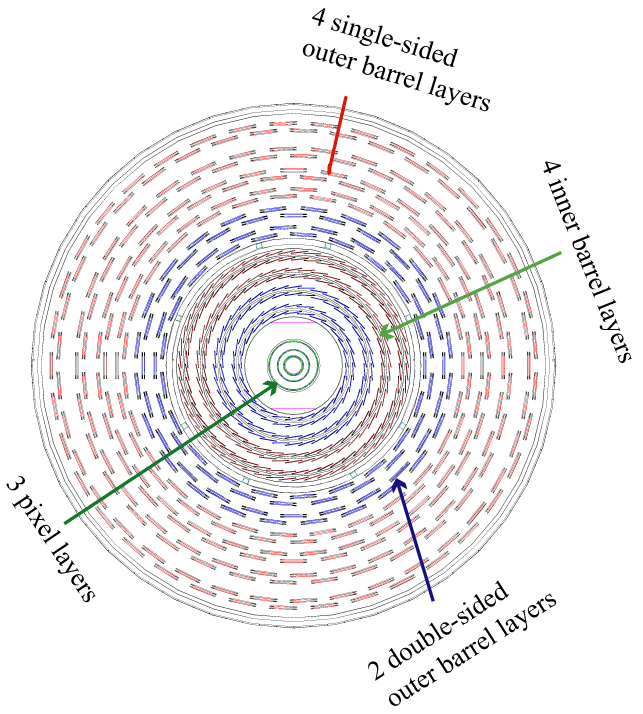
\includegraphics[width=360pt]{Figures/tracker-Barrel.png}
    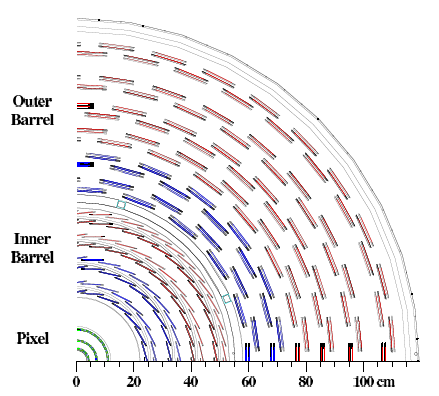
\includegraphics[width=360pt]{Figures/tracker-schematic.png}
  \end{center}
  \caption[\fixspacing Diagram of layers in tracker barrel]
	  {\fixspacing Diagram of layers in tracker barrel.}
  \label{fig:TrackerBarrel}
 \end{figure}

\subsection{Calorimeters}
\label{exp:cal}
The general purpose of a calorimeter 
is to measure energy passing through it.  
CMS measures %the energy of decay products 
particles' energies 
with a scintillating electromagnetic calorimeter (ECAL),
situated just outside the tracker,
and a sampling hadronic calorimeter (HCAL),
surrounding the ECAL.  
Both calorimeters are contained within the solenoid.  
This solves a problem seen in other detector designs, 
in which energy lost in the magnet material leads 
to an uncertainty in the energy measurement.  

\subsubsection{ECAL}
\label{exp:ECAL}
The ECAL is made up of \~76,000 lead tungstate crystals,
arranged in a cylindrical barrel and disk-shaped endcap geometry.  
The barrel is divided into 18 sections in $\phi$ and 
two in $\eta$, called supermodules.  
Each endcap is divided into two half-disks, called dees.  
Each lead tungstate crystal is 
2.2 cm x 2.2 cm wide and 23 cm long for the barrel, 
and 3 cm x 3 cm wide and 22 cm long in the endcap.  
The dimensions were chosen such that the width 
of each crystal is approximately the characteristic size of 
an electromagnetic shower within it 
(Moliere radius of 2.19 cm),
and the length is \~25 times the radiation length 
of the material (0.89 cm for lead tungstate).  
In the barrel, the crystals are oriented with the long axis
directed towards the interaction point.  
However, to avoid particles being lost in the cracks 
between the crystals,
the crystals are offset by 3 degrees in both the 
$\phi$ and $\eta$ directions.  
An electromagnetically-interacting particle will 
induce a shower inside the crystals, 
and the resulting light is captured by 
photodetectors situated at the back of each crystal.  
The energy resolution was measured to be 
\[
%INSERT LONG FUN EQUATION FROM P.120(147) OF DETECTOR PAPER HERE
\left(\frac{\sigma}{E}\right)^2 = \left(\frac{2.8\%}{\sqrt{E}}\right)^2 + \left(\frac{0.12}{E}\right)^2 + \left(0.30\%\right)^2
\]

A preshower detector, consisting of lead radiators 
and silicon sensors, 
is situated on the face of each endcap.  
The preshower serves to identify electron pairs due to low-energy 
pion decays and differentiate them from more 
interesting signatures.  
Pions typically decay on the scale 
of the distance between the interaction point and the 
ECAL endcap;
therefore there is no preshower detector for the barrel, 
which is too close to the interaction point.  

\subsubsection{HCAL}
\label{exp:HCAL}
%HCAL resolution of energy: CMS NOTE 2006/036, but it's only
%MC and also not just one equation.  can give value
%quoted in abstract.  also, incl ecal: it's for reco jets
%OR can take value from prelim, but don't remember where it came
%from: look in HCAL TDR
%ORRRR: not important because not in detector paper, and
%couldn't find it in tdr? (which is confusing in any case)
The hadronic calorimeter surrounds the ECAL and 
covers $|\eta| < 3$ in the barrel and endcap (HB/HE) 
and up to $|\eta| < 5$ in the forward calorimeter (HF),
both within the magnet coil.
Additionally, the outer calorimeter (HO) is situated 
outside the solenoid and serves to detect 
and measure any leak-through.
In general HCAL uses sampling calorimeter technology, 
with brass and scintillator layers interleaved 
in the barrel and endcap, 
and steel plates and quartz fibers for HF; 
quartz was used in the forward region 
because of its ability to 
withstand very high particle fluxes.  
In a sampling calorimeter, the layers of metal absorber 
induce particle showers, which are then 
``sampled'' by the layers of scintillator 
attached to photodetectors.  
Not all of the energy is directly detected, 
some being lost in the metal,
so the energy measurement is scaled using 
experimentally-determined factors.  
The depth of the HCAL 
in terms of interaction length 
varies between 5.82 $\lambda_I$ at $\eta = 0$ and 
10.6 $\lambda_I$ at the edge of HB and throughout 
the endcap, 
with the ECAL adding 1.1 $\lambda_I$.  
The HO extends the HCAL depth to at least 
11.8 $\lambda_I$ in the barrel, 
with the magnet material acting as the absorber for 
the HO scintillator layer.  
(An additional layer of iron and 
a second scintillator exist
at the $\eta = 0$ ring, 
where the HB depth is the least.)
Since there is no ECAL in the forward region, 
the HF is equipped to distinguish electromagnetic 
objects from hadronic jets with different 
lengths of quartz fibers.  
The long fibers reach the entire depth of HF, 
while the short fibers only start halfway through 
the detector.
Since electromagnetic showers tend to occur in the 
first half of the detector, 
and hadronic showers throughout the full HF, 
a shower detected only by the long fibers 
is likely to be electromagnetic in nature.  

\subsection{Muon System}
\label{exp:muons}
The CMS muon system serves to identify muons, 
which are the only particles that leave a signature 
very far from the interaction point,
and also to measure their momentum.  
The system is situated outside the magnet coil, 
within the iron return yoke, 
and provides coverage up to $|\eta| < 2.4$.  
The return yoke also functions as an absorber 
to filter out backgrounds to the muon signal.  
The muon system consists of three separate subsystems: 
drift tube chambers (DTs) in the barrel up to $|\eta| < 1.2$, 
cathode strip chambers (CSCs) in the endcap 
with an $\eta$ range $ 0.9 < |\eta| < 2,4$, 
and resistive plate chambers (RPCs) %providing redundancy 
in the region $ |\eta| < 1.6$.  

The DTs are used in the barrel due to 
relatively low muon rates in this area, 
in addition to a uniform magnetic field in the 
return yoke.  
Four stations of chambers are interspersed 
within the iron frame to form % within instead of with -- Wesley
concentric cylinders around the beam pipe, 
with a total of \~172,000 detection wires.  
Orthogonal positioning of the wires 
within each chamber provides measurement of 
both azimuthal and longitudinal position.  
Each wire detects charge that drifts toward it 
due to an applied voltage when a muon ionizes 
the surrounding gas, as illustrated in 
Figure \ref{fig:DTconcept}.  
Neighboring chambers overlap 
to ensure full coverage.  

 \begin{figure}[htb]
  \begin{center}
    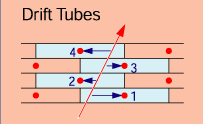
\includegraphics[]{Figures/muon-DT-concept.png}
  \end{center}
  \caption[\fixspacing Conceptual diagram of drift tube chambers]
	  {\fixspacing Conceptual diagram of drift tube chambers.}
  \label{fig:DTconcept}
 \end{figure}

The CSCs are used in the endcap, 
where the muon rate and overall particle flux 
are higher.  
Cathode strips in each chamber 
measure the $\phi$-position of a hit, 
while anode wires oriented perpedicularly measure 
the $\eta$-position.  
There are on the order of 200,000 readout channels 
for each type of measurement.  
Four stations of CSCs are used in each endcap; 
each muon in the range $1.2 < |\eta| <2.4$ crosses either 
3 or 4 stations.  
For $|\eta|$ between 0.9 and 1.2, muons are detected 
both by the CSCs in the endcap and the DTs in the barrel.  
Coverage is provided by overlapping layers of chambers 
at each station.  

 \begin{figure}[htb]
  \begin{center}
    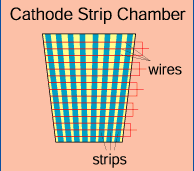
\includegraphics[]{Figures/muon-CSC-structure.png}
  \end{center}
  \caption[\fixspacing Diagram of cathode strip chamber]
	  {\fixspacing Diagram of cathode strip chamber, 
	    showing the cathode strips and anode wires 
	    for measuring the $\phi$ and $\eta$ coordinates, respectively.}
  \label{fig:CSCstructure}
 \end{figure}

The RPCs provide redundancy for the previous 
two systems as well as a faster response time 
in place of a highly accurate position measurement.  
The RPCs measure the timing of a hit with a 
1 ns resolution, compared to the 25 ns LHC bunch spacing 
and hundreds of ns drift time in the drift chambers.  
Six layers of RPCs are interspersed with the 
drift tubes in the barrel, 
while three layers are used in the endcap 
with the CSCs.  
Again, overlapping chambers ensures full coverage.  
Each chamber consists of two or three double-gap 
modules, each of which has a single readout module 
between two thin gas chambers.  
The readout module consists of metal strips, 
which capture the electric charge created when 
a muon ionizes the gas, causing an avalanche of charge.  
Figure \ref{fig:RPClayers} shows a diagram of the structure.  

 \begin{figure}[htb]
  \begin{center}
    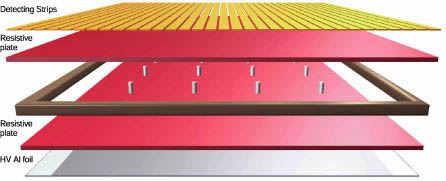
\includegraphics[width=360pt]{Figures/muon-RPClayers.jpg}
  \end{center}
  \caption[\fixspacing Diagram of resistive plate chamber]
	  {\fixspacing Diagram of resistive plate chamber.}
  \label{fig:RPClayers}
 \end{figure}

Overall, the muon system has a momentum resolution 
of 9\% for relatively moderate-$p_T$, low-$\eta$ muons, 
and ranging from 15\% to 40\% for very-high-$p_T$ muons.  
When combined with the information from the inner tracker, 
however, this resolution improves to \~1\% and 5\%, respectively.  

\subsection{Trigger}
\label{exp:trigger}
The purpose of the CMS trigger is to 
identify potentially interesting events.  
Storing the data from every collision is unfeasible; 
resources allow only a very small fraction of events to be kept.  
Therefore the trigger reduces the effective event rate, 
keeping only the events with an interesting signature, 
for example a large energy deposit.  
There are two levels to the CMS trigger.  
The Level-1 Trigger uses hardware-implemented algorithms to 
reduce the event rate from the LHC collision frequency of 40 MHz 
to a maximum of 100 kHz; 
this must be done quickly since the initial event rate is high. 
The High-Level Trigger reduces the rate further to \~200 Hz, %(OR 100??)
using a computer farm to process each event in more detail; 
having a lower input rate, it can afford more processing time per event.  

%Picture: Overall diagram of trigger

\subsubsection{Level-1 Trigger}
\label{exp:L1}
%General L1 information, specific electron algorithms in online selection section.  
%time-of-flight stuff!

The Level-1 trigger (L1) \cite{TriggerTDR} 
uses mostly programmable, hardware-based algorithms 
to identify and roughly reconstruct possibly interesting physics objects, 
such as electrons and muons.  
This is done within 3 $\mu$s.  
The structure of the L1 is shown in Figure \ref{fig:L1Structure}.  
Parallel chains process the muon system and calorimeter objects separately. 
Tracking information is not included in the L1, 
which means the L1 algorithms do not distinguish 
between electrons and photons. 
%Subsections on that?  Need to talk about the muon parts, as well as the multi-level calo part.  
The first step of the Level-1 trigger is the generation 
of coarse versions of the readout information 
from each of the muon and calorimeter channels; 
this information is called trigger primitives.  
The trigger primitives are passed to regional trigger systems, 
which combine them into trigger objects.  
The objects for each region are then passed to a global system, 
which picks out the highest-energy (and therefore most interesting) 
objects of each type.
The final set of objects gets passed on to the last level, 
the global trigger, which combines information from both 
the calorimeter and muon chains 
and makes a single decision based on the set of criteria implemented.  
%(Ooh boy, go back to RT2010 stuff!)  

The trigger system must combine all the pieces of information 
according to which bunch crossing they originate from.   
This is complicated by the fact that the time it takes particles 
to reach the outer edge of the muon system 
is 
%about 
more than % Wesley
that of the bunch crossing interval.  
In addition, the cable lengths between the subdetectors 
and the trigger subsystems and within the trigger are 
all different, 
and each of the trigger systems has a different processing time.  
Despite these challenges, the timing of each piece of 
the L1 trigger has successfully been tuned to keep everything running 
synchronously.  

%(from ecal section) PICTURES OF SUPERMODULE GEOMETRY -- maybe just for trigger section?

%nice picture of L1 architecture from detector paper

 \begin{figure}[htb]
  \begin{center}
    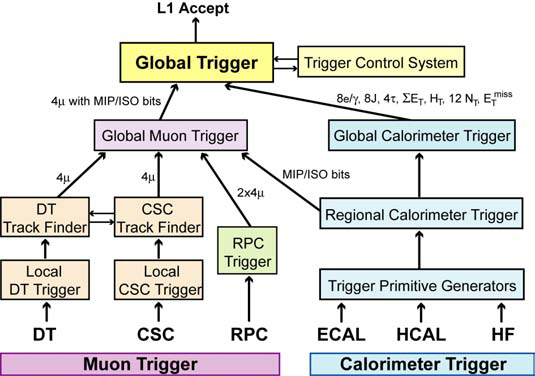
\includegraphics[width=360pt]{Figures/L1structure.png}
  \end{center}
  \caption[\fixspacing Structure of the Level-1 trigger]
	  {\fixspacing Structure of the Level-1 trigger.}
  \label{fig:L1Structure}
 \end{figure}

\subsubsection{Regional Calorimeter Trigger}
\label{exp:RCT}
The Regional Calorimeter Trigger (RCT) \cite{rctTriggerSystem}
was designed and built and is maintained 
by the University of Wisconsin at Madison.  
It sits in eighteen crates in nine racks in the CMS underground electronics room.  
Each crate deals with one slice of $\eta$-$\phi$ space.  
The general purpose of the RCT is to take 
energy information from ECAL and HCAL and combine it 
to generate electron/photon candidates as well as energy sums for 
jet-finding.  
A diagram illustrating the structure of the RCT processing 
is shown in Fig.~\ref{fig:RCTStructure}.  

\begin{figure}[htb]
  \begin{center}
    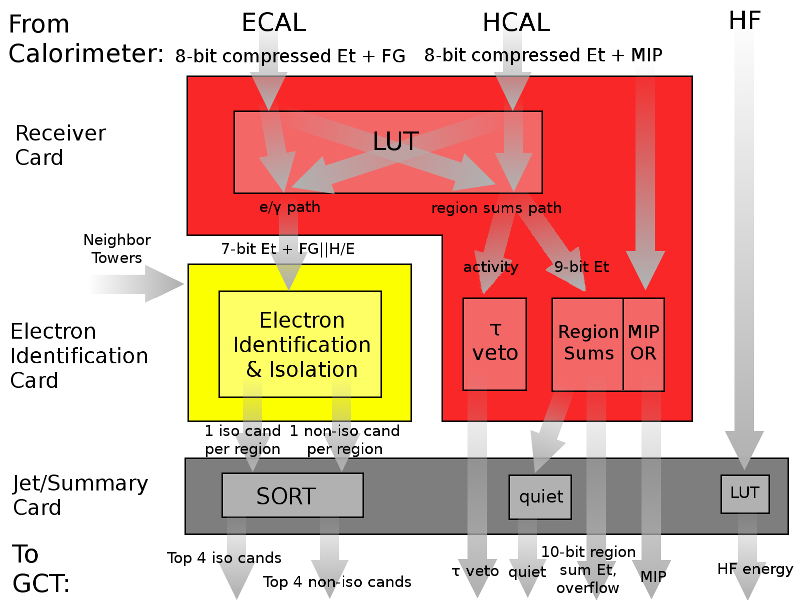
\includegraphics[width=400pt]{Figures/RCT-structure-new-small.png} 
  \end{center}
  \caption[\fixspacing Diagram of the RCT structure]
	  {\fixspacing Diagram of the RCT structure.
	    The RCT (Regional Calorimeter Trigger) takes energy 
	    information at the tower level from the electromagnetic 
	    and hadronic calorimeters.  
	    It processes this information to produce 
	    regional energy sums, electron candidates, 
	    and other regional information to be 
	    used in the GCT (Global Calorimeter Trigger) 
	    processing further downstream.
	  }
	  \label{fig:RCTStructure}
\end{figure}

The information from the calorimeters arrives at the level of trigger towers, 
a larger granularity than that sent to the full readout.  
Each ECAL tower corresponds to an HCAL tower behind it.  
For each ECAL+HCAL tower, the RCT uses memory lookup tables (LUTs) to 
calculate the total energy sum 
as well as the ratio of HCAL energy to ECAL energy.  
If that ratio is higher than a certain value, 
too much energy has been deposited in the HCAL tower for it to 
contain a probable electron or photon.  
The electron/photon candidates are constructed starting from 
towers whose energy deposit is higher than any of their 
four immediate neighbors.  
This primary tower must not have the ECAL fine grain bit set; 
this fine grain bit indicates a structure in the energy deposit 
inconsistent with an electron or photon.  
The tower's energy is then combined with that of its highest-energy 
neighbor, to account for particles that deposite energy 
in more than one tower; 
this is the energy of the candidate.  
The candidate is then determined to be either ``isolated'' or 
``non-isolated'' depending on the character of the deposits 
in the neighboring towers.  
If the eight towers forming a square around the primary tower 
have two full sides (five contiguous towers) with 
deposits below a configurable threshold (the ``quiet'' threshold), 
and these towers' fine grain bits are not set, 
then the candidate is isolated.  
Otherwise, it is non-isolated.  
The algorithm is illustrated in Figure~\ref{fig:RctEgAlgo}.  
Each crate sorts the isolated and non-isolated candidates found 
according to energy, 
and the four highest-energy of each type are kept and passed on.  

 \begin{figure}[htb]
  \begin{center}
    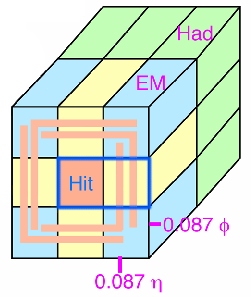
\includegraphics[width=240pt]{Figures/RCT-EG-algo.png} 
  \end{center}
  \caption[\fixspacing Diagram of the RCT electron/photon algorithm]{
    \fixspacing Diagram of the RCT electron/photon algorithm. 
    The candidate is defined as a tower whose four 
    immediate neighbor towers have lower energies.  
    The candidate tower's energy is combined with 
    the energy of its highest-energy neighbor.  
    The candidate is defined as ``isolated'' if 
    five contiguous towers out of the eight 
    surrounding it (two full sides of the square) 
    have energies below a ``quiet'' threshold 
    and do not have the fine grain bit set.  
    Otherwise the candidate is ``non-isolated.''  
  }
  \label{fig:RctEgAlgo}
 \end{figure}

The RCT also calculates the total energy sums 
of square regions of the calorimeter, 
4 trigger towers to a side.  
The topology of the energy deposits in each region 
is examined to determined whether or not the 
deposit is consistent with that from 
a $\tau$ particle that has decayed hadronically, 
i.e. decayed into a jet of hadrons.  
Only deposits above a configurable threshold 
are considered.  
If the deposits in the region make up a 
single, small, contiguous area as shown in 
Figure~\ref{fig:RctTauAlgo},
then they are consistent with a tau.  
In this case the $\tau$ veto bit associated 
with the region is set to false; 
in all other cases, it is set to true.  
In addition, the HCAL sends a bit for each 
HCAL tower indicating whether the deposit 
is consistent with a minimum ionizing particle 
(MIP) or muon.  
If any individual tower's MIP bit is true, 
then the overall MIP bit associated with the region 
is also set to true.  
Otherwise it is set to false.  

 \begin{figure}[htb]
  \begin{center}
    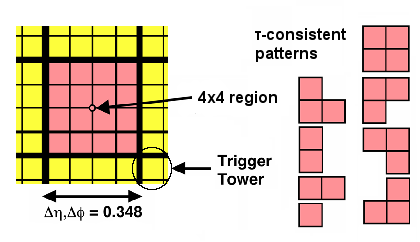
\includegraphics[width=400pt]{Figures/RCT-tau-algo.png} 
  \end{center}
  \caption[\fixspacing Diagram of the RCT $\tau$ algorithm]{
    \fixspacing Diagram of the RCT $\tau$ algorithm. 
    The energy deposits in each region are 
    examined to determine whether they are 
    consistent with that from a $\tau$ 
    that has decayed hadronically.  
    A single small, contiguous region 
    is consistent with a $\tau$. 
  }
  \label{fig:RctTauAlgo}
 \end{figure}

Finally, the RCT sends the regional energy sums 
and the list of possible 
electrons or photons, 
along with the associated bits (MIP, $\tau$), 
to the 
Global Calorimeter Trigger (GCT) level.  
The GCT groups the regional energy sums into jets 
and collects the four highest-energy isolated and 
non-isolated electron/photon candidates, 
and sends this information to the Global Trigger (GT), 
the last step in the chain.  
The Global Trigger makes the final decision on 
whether to accept or reject an event at the Level-1.  
% NEED THE GCT/GT stuff?  talked about it earlier a little


\subsubsection{High-Level Trigger}
\label{exp:HLT}
%General HLT information, specific electron algorithms in online selection section.  

The High-Level Trigger (HLT) \cite{hlt-0512077} 
is implemented on a computer farm in the 
CMS above-ground control room building.  
It serves to reduce the L1 output event rate from \~100 kHz to a rate suitable 
for transfer and storage to disk, around 200 Hz.  
An event must pass the HLT to be analyzed offline.  
The input rate at this stage is lower than that at the Level-1, 
so more time can be 
%afforded to spend 
spent % Wesley
on the decision, 
and more detailed reconstruction can be done.  
The HLT uses versions of the standard offline physics-object reconstruction algorithms 
optimized for fast performance.  
The algorithms need to be more accurate than those of the L1, 
but absolute accuracy at the offline reconstruction level is not necessary.  
Still, the HLT algorithms are kept as close to the offline ones as possible.  
Specific algorithms are dealt with in more detail in 
%a later chapter.  
Section~\ref{evSel:HLT}.  

\subsubsection{Trigger Menus}
\label{exp:trigMenus}
Both the L1 and High-Level Triggers use the concept of a trigger menu.  
There are different sets of criteria defining an ``interesting'' event 
at any one time;  
each set of criteria is called a trigger path.  
When an event fulfills all the criteria for a given path, 
that path ``fires'' and the event is accepted.  
Some paths may fire at a higher rate than desired, 
so a prescaling factor is implemented: 
only a fraction of events firing that path is kept.  
For example, a path with a prescale of 5 only 
has 1/5 of its passing events actually saved.  
In this way, events passing a certain path can still 
be studied without taking too much of the available resources.  
The set of paths that are being checked at any given time,
along with their prescale factors,  
is called the trigger menu.  
The Level-1 and High-Level Triggers each have their own 
trigger menus.  
Since the L1 must do things quickly, 
its criteria are simple, 
whereas the HLT may have more complex criteria.  
Passing a given L1 path causes 
related HLT paths to be run on that event.  

%algorithms evolve with luminosity
At the beginning of collision running, 
the event rate was low enough to allow very loose trigger 
menus to be used.  
At the HLT, a ``keep-everything'' pass-through menu 
recorded essentially all activity.  
As the luminosity increased, however, more stringent criteria had 
to be applied to maintain an acceptable event rate, 
for example, raising the amount of energy needed to accept an 
``interesting'' object.  
The successive algorithms have been studied in detail and 
commissioned successfully throughout the 2010 running conditions.  

\subsection{Luminosity}
\label{exp:lumi}
%How the luminosity is measured (definition? or that done earlier in general particle physics section? recap here?)
%What's actually used: HF?? that's in the detector paper, but not much else.  go to twiki, I guess (and that HN thread)

CMS measures luminosity with the forward calorimeter, which sits 
between $|\eta|$ of 3 and 5, close to the beam pipe.  
Two different methods of measurement are used.  
The first method counts the number of occupied towers in the HF 
(above some energy threshold to avoid noise), 
using the principle that that number is proportional to the luminosity.  
However, at high luminosity the number of occupied towers may begin to 
saturate, making this method less accurate.  
The second method does not saturate in this way: 
it measures the total energy deposited in the HF, 
which is also proportional to the luminosity.  
The information from both of these methods is combined into one 
luminosity value.  

Fig. \ref{fig:LuminosityVsTime} shows the total integrated luminosity at CMS 
as a function of time for the 2010 running period \cite{LumiPublicResults2010}.  
The amount of data validated for physics analysis was 
%36.1 $pb^{-1}$.  
36.1 \pb.  

 \begin{figure}[htb]
  \begin{center}
    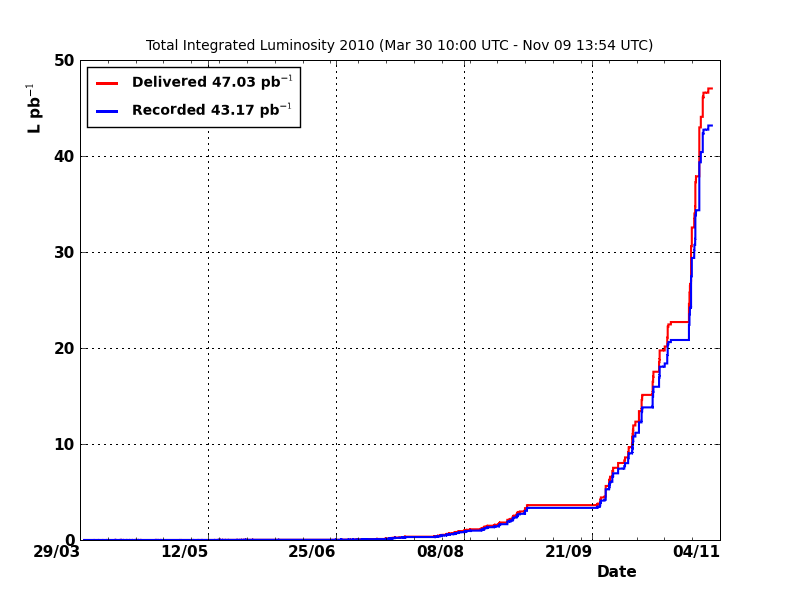
\includegraphics[width=360pt]{Figures/totallumivstime2010.png}
  \end{center}
  \caption[\fixspacing Luminosity collected by CMS as a function of time, 2010]
	  {\fixspacing Luminosity collected by CMS as a function of time, 2010.}
  \label{fig:LuminosityVsTime}
 \end{figure}

% need the DAQ someplace??  online event selection?  or don't really need it?
% really don't need too much in the way of specifics, methinks


\chapter{Event Simulation}
\section{Monte Carlo Event Generation}
\subsection{some explanation of the black box}
\subsection{Monte Carlo Generators}
\subsubsection{PYTHIA}
\subsubsection{POWHEG}
\section{Detector Simulation}
%\subsection{GEANT Detector Model/Modeling of Particle Interactions in Detector Material}
\subsection{GEANT Detector Model}
\subsection{Level-1 Trigger Emulator}

\chapter{Event Reconstruction}
\label{evReco}
%a little on daq, event building here?

%Only dealing with parts of event relevant to \Zee analysis.  

The information from the detector for any given event 
gets read out over millions of channels 
from the many different subdetectors.  
These signals must be combined to provide 
meaningful physics information 
%that can be analyzed
about the interaction that took place 
within the detector, 
namely the measurable quantities 
(like direction and energy) 
of the outgoing decay products.  

\section{Detector Object Reconstruction}
\label{evReco:detReco}
%This is for the basic objects only. 
%BUT, basic object reconstruction is so integrated with 
%physics object reconstruction, maybe combine them?

The first step of the particle reconstruction 
involves translating the information from each 
detector channel, 
such as position and electronics signal, 
into useful quantities such as position in 
$\eta$-$\phi$ space and energy or momentum.  
This is done by algorithms 
mapping each individual 
detector cell to its $\eta$-$\phi$ placement 
and calculating its energy, 
which necessarily takes into account 
the position of each cell.  
The second step involves 
connecting information from different channels 
to build up a more complex picture of 
the particles that passed through the detector.  

\subsection{Electromagnetic Calorimeter Reconstruction}
\label{evReco:ECAL}
%\subsection{Electromagnetic Calorimeter Clustering}
%reconstruction of position of energy deposits, 
%rechits and that stuff: digitization, calibration?
% where to go for this stuff?? well, reco principles or
% ecal local reco to start...

The information coming directly from the ECAL 
is read out in terms of each cell's electronics response.  
The ECAL reconstruction algorithms translate this into 
an energy value, which is then calibrated 
according to the cell's energy %as well as its 
and 
$\eta$-position.  
The algorithms also calculate quantities 
relevant to the quality of the deposit, 
in particular whether or not the deposit happened 
at a time consistent with the LHC 
bunch collisions, i.e. if it was ``in time'' or ``out of time''.  
%bunch collisions, i.e. if it was ``in time''.  
This information is especially useful in 
identifying apparent energy deposits that have 
been found to come from the 
%electronics themselves; 
signal-conversion electronics theselves (the transducers); % Wesley
these fake deposits were discovered during 
commissioning and are known as ``ECAL spikes''.  
Since the spikes can imitate energy deposits from 
actual 
%decay products, 
particles, % Wesley
they must be removed from the information used 
to reconstruct electrons and other particles.  
They can be distinguished from real particle deposits 
due to their timing 
as well as the fact that the surrounding crystals 
have no trace of a deposit.  
Therefore, if a high-energy deposit has no or 
very little energy in its neighboring crystals, 
or if its timing is not consistent with a bunch 
crossing, 
it is considered a spike and taken out of the 
reconstruction.  

%\subsubsection{ECAL Spike Removal}
%ALSOOOOO need to talk about spikes and spike removal
%(since that's now automatic, but also wasn't previously. 
%then talk about in event selection, because that was 
%a criterion...? no, because it's not a criterion for 
%e.g. newest datasets)
% HAVEN'T FOUND REFERENCE FOR WHAT'S INCLUDED IN RECO
% except for, like, swiss cross and out of time, is that enough?

%\subsection{Pixel Hits} % need?

\subsection{Track Reconstruction}
\label{evReco:track}
A track is a sequence of hits in the tracker, 
reconstructed to trace the trajectory of a passing 
particle.  
The Kalman Filter algorithm is used by default for CMS tracks, 
but is not good at catching abrupt changes in the 
electron trajectory due to bremsstrahlung.  
Therefore, the Gaussian Sum Filter algorithm 
is used for electrons, 
because it is able to find 
those hits in unexpected directions.  

\subsubsection{Kalman Filter}
\label{evReco:KF}
% CMS Note 2006/041
% CMS Note 2006/026 for seeding
The Kalman Filter (KF) tracking method \cite{CMS-NOTE-2006-041} 
is seeded \cite{CMS-NOTE-2006-026}
by pairs of hits in the pixel detector.  
The seeding algorithm first searches for a hit 
in one of the outer layers of the pixel detector.  
If a hit is found, another hit is sought in a 
layer closer to the interaction point, 
looking in an $\eta$-$\phi$ window around 
the original hit.  
Only two out of the three pixel layers are 
required to have hits 
in order to maintain a high efficiency.  
Once a track seed is found, 
further hits are sought in each successive tracking layer. 
The Kalman filter method is used to predict possible 
locations for hits in the next layer based on 
the currently-known track parameters. % and their 
%uncertainties.  
Hits in that area are then sought and included 
in the track, combining each hit with the 
predicted location for that layer and weighting 
each value depending on the value's uncertainty.  
If there are multiple candidate hits in the next layer, 
a possible trajectory is calculated for each hit, 
along with a trajectory accounting for the case 
in which the hit in that layer was lost.  
This procedure is repeated for each layer: 
each of the calculated trajectories for a given layer 
is matched to hits in the next layer, 
for which new trajectories are calculated.  
To prevent the number of necessary calculations 
from growing too large, 
the number of possible trajectories at each step 
is capped at five.  
%(BUT HOW DETERMINED WHICH ONES???)
%at each layer
In the case of multiple possible trajectories 
for a given fully-reconstructed track, 
defined by two trajectories sharing more than 
half of each of their hits,
the track candidate with fewer hits 
(or, in the case of the same number of hits, 
the track with the worse fit)
is discarded.  

\subsubsection{Gaussian Sum Filter}
\label{evReco:GSF}
% CMS Note 2005/001

The Kalman Filter track-fitting does not accurately 
account for the behavior of particles in a material, 
specifically energy lost in the material 
and changes in direction due to radiation.  
The KF description is in particular inadequate 
for electrons, which 
readily interact with matter in these ways.  
%are prone to these interactions with matter.  
The Gaussian Sum Filter (GSF) algorithm 
\cite{CMS-NOTE-2005-001} was 
therefore developed:
essentially a Kalman Filter 
with a more sophisticated energy loss modeling.   
Instead of approximating the energy loss 
(which is non-Gaussian)
with a Gaussian distribution, 
which KF implicitly does, 
the GSF method models it as a 
weighted sum of Gaussian distributions.  
This greatly improves the performance 
of the track-fitting for electrons.  
%PICTURE? trk-gsf-QoverP.png shows charge-to-momentum
% ratio for KF and GSF -- but figure out 
% WHAT Q/P ACTUALLY TELLS YOU

\section{Electron Reconstruction}
\label{evReco:elec}
% https://twiki.cern.ch/twiki/bin/view/CMS/ElectronRecoPrinciples
% https://twiki.cern.ch/twiki/bin/view/CMS/SWGuideEcalRecoClustering
%here's where we start talking about electrons
%CMS Note 2006/040
As an electron 
%from an interaction 
passes through the CMS detector, 
it leaves a signature pattern in the subdetectors.  
Characteristically, electrons produce a track 
in the tracker system, 
as well as an energy deposit in the 
electromagnetic calorimeter.  
Therefore an electron is reconstructed 
by matching tracks and energy clusters 
that appear to have been made by the same particle 
\cite{CMS-NOTE-2006-040}.  
There are currently two approaches used to 
initiate electron reconstruction: 
the ``ECAL-driven'' method and 
the ``tracker-driven'' method, 
named according to which subdetector's 
information initiates the reconstruction.  
%one starts with ECAL information 
%while the other begins with information from 
%the tracker.  
Each method produces a collection of 
basic electron candidate objects, 
each consisting of a calorimeter cluster 
and hits in the first few layers of the tracker.  
These collections are then combined into one 
and used as seeds to reconstruct the electron tracks, 
producing fully-reconstructed electrons.  
%how many electrons are one vs other vs both?

\subsection{ECAL-driven Electron Seeding}
\label{evReco:ecalDrv}

The ECAL-driven electron reconstruction method 
starts with an energy deposit (or ``supercluster'') 
in the ECAL 
and searches for hits in the 
pixel system that matches the 
position of the calorimeter deposit.  

\subsubsection{Superclusters}
\label{evReco:SC}
%Hybrid and multi5x5 (hybrid doesn't start with basic clusters, 
%so probably combine detector object and physics object sections)

The calorimeter energy deposit used in the electron 
reconstruction is called a supercluster: 
a cluster of clusters.  
A single electron or photon deposits most of its energy 
in a 5x5 square of ECAL crystals, 
as shown in Fig. \ref{fig:BasicCluster}.  
However, an electron passing through the tracker material 
in a strong magnetic field produces 
bremsstrahlung and electrons from converted photons, 
causing the original electron's energy to 
have spread out in $\phi$ once it reaches the calorimeter.  
The process of creating a supercluster gathers these 
energy deposits to form the initial energy of the electron.  

 \begin{figure}[htb]
  \begin{center}
%    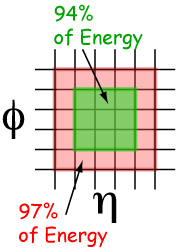
\includegraphics[width=360pt]{Figures/elec-BasicCluster-opaque.png}
    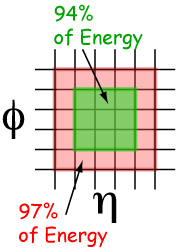
\includegraphics[width=180pt]{Figures/elec-BasicCluster-opaque.png}
  \end{center}
  \caption[\fixspacing Typical energy distribution in a basic cluster]
	  {\fixspacing Typical energy distribution in a basic cluster.}
  \label{fig:BasicCluster}
 \end{figure}

% need pretty picture!

The electron reconstruction currently uses two different 
superclustering methods, 
the ``hybrid'' supercluster method in the barrel, 
and the ``multi5x5'' clustering method in the endcap.  
The hybrid algorithm forms superclusters 
and basic clusters from the same energy deposit 
information, 
while the multi5x5 algorithm first forms 
a single collection of basic clusters, 
which are then separately combined into superclusters.  

%Hybrid
%``hybridSuperClusters''
%hybrid: (dynamic phi road turned OFF)
%http://cmssw.cvs.cern.ch/cgi-bin/cmssw.cgi/CMSSW/RecoEcal/EgammaClusterProducers/python/hybridSuperClusters_cfi.py?revision=1.10&view=markup
%http://cmssw.cvs.cern.ch/cgi-bin/cmssw.cgi/CMSSW/RecoEcal/EgammaClusterProducers/src/HybridClusterProducer.cc?revision=1.32&view=markup
%http://cmssw.cvs.cern.ch/cgi-bin/cmssw.cgi/CMSSW/RecoEcal/EgammaClusterAlgos/src/HybridClusterAlgo.cc?revision=1.61&view=markup


The hybrid algorithm starts with a list of all 
ECAL crystals with an energy greater than a threshold; 
these crystals are considered seeds.  
Beginning with the highest seed crystal, 
the area around each seed is searched for 
energy deposits in steps of one crystal in $\phi$.
For each $\phi$ step, a ``domino'' of crystals is 
formed in $\eta$: 
one crystal to each side of the central crystal, 
or, if the energy sum of those three crystals is 
greater than a threshold, 
two crystals to each side of the central crystal, 
for a total of five crystals per domino.  
The process is done for a given number of $\phi$ 
steps in both the positive and negative directions 
(currently 17 steps).  
As other seeds are encountered in this process, 
they are removed from the list of available seeds.  
Each domino with a higher energy than its two neighbors 
is considered as the seed for a basic cluster, 
and the collection of dominos formed by the search 
process is the basis for the supercluster.  
The basic clusters are formed by summing the 
energy of each local-maximum domino with 
those of its neighboring lower-energy dominos, 
excluding dominos that have already been used.  
The supercluster is then formed by summing the energies 
of the constituent basic clusters, 
with its seed considered to be the highest-energy 
basic cluster 
and its position given by the energy-weighted positions 
of the constituent clusters.  
%PICTURE

%Multi5x5:
%``multi5x5SuperClustersWithPreshower''

%https://twiki.cern.ch/twiki/bin/view/CMS/ECALDPGClusterization  also talks about supercluster energy corrections
%http://cmssw.cvs.cern.ch/cgi-bin/cmssw.cgi/CMSSW/RecoEcal/EgammaClusterProducers/python/multi5x5SuperClusters_cfi.py?revision=1.2&view=markup
%http://cmssw.cvs.cern.ch/cgi-bin/cmssw.cgi/CMSSW/RecoEcal/EgammaClusterProducers/src/Multi5x5ClusterProducer.cc?revision=1.5&view=markup
%http://cmssw.cvs.cern.ch/cgi-bin/cmssw.cgi/CMSSW/RecoEcal/EgammaClusterAlgos/src/Multi5x5ClusterAlgo.cc?revision=1.9&view=markup
%http://cmssw.cvs.cern.ch/cgi-bin/cmssw.cgi/CMSSW/RecoEcal/EgammaClusterProducers/src/Multi5x5SuperClusterProducer.cc?revision=1.2&view=markup
%http://cmssw.cvs.cern.ch/cgi-bin/cmssw.cgi/CMSSW/RecoEcal/EgammaClusterAlgos/src/Multi5x5BremRecoveryClusterAlgo.cc?revision=1.8&view=markup SCORE

The multi5x5 algorithm first creates a collection 
of basic clusters from seeds, 
which are ECAL crystals with an energy higher than 
a given threshold.  
If a seed represents a local maximum, 
then its energy deposit is combined with those 
from the crystals in the surrounding 5x5 square 
to form a basic cluster, 
ignoring any crystals that have already been 
used to form the central 3x3 part of another cluster.  
The basic clusters are then used as seeds for the 
superclustering algorithm.  
For each seed cluster with energy higher than a threshold, 
the energies of any other clusters within an $\eta$-$\phi$ 
window of the seed (longer in $\phi$ than in $\eta$)
are combined with its own energy to create the supercluster, 
leaving out clusters that have already been used to 
form another supercluster. 
The position of the supercluster is given by the 
energy-weighted position of the individual clusters.  

%also preshower cluster info in endcap... how?
%what kind of energy corrections done? 
%or is that for energy scale section?
%at least SC corrections are in dpg clusterization twiki

\subsubsection{Pixel Hit-matching}
\label{evReco:pixMatch}

To reconstruct the full electron, 
the supercluster must be matched with a track.  
% where exactly to split ecal-driven and tracker-driven?
This is done by extrapolating the probable position of 
tracker hits from the supercluster's position, 
%given the supercluster energy.  
as illustrated in Fig. \ref{fig:PixMatch}.  
Given the supercluster energy and the fact that a 
non-radiating electron would have hit the calorimeter 
at the energy-weighted center of the supercluster's 
energy spread, 
the electron's initial (pre-radiation) trajectory 
through the tracker can be calculated 
for both the positive and negative electron 
charge cases.  
The reconstruction algorithm then looks for a matching 
hit in the first pixel detector layer 
within a $\phi$-$z$ window of this position 
for each charge case.  
If a hit is found, another hit is sought in the second 
pixel layer within a different $\phi$-$z$ window 
of the hit in the first layer.  
%This set of pixel hits is the seed(??)

%PICTURE from my old talk or something!  

 \begin{figure}[htb]
  \begin{center}
%    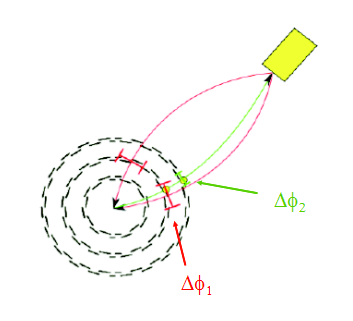
\includegraphics[width=360pt]{Figures/elec-pixmatch.png}
    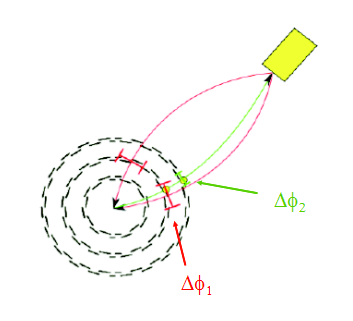
\includegraphics[width=240pt]{Figures/elec-pixmatch.png}
  \end{center}
  \caption[\fixspacing Schematic of pixel-hit search algorithm in electron-seeding]
	  {\fixspacing Schematic of pixel-hit search algorithm in electron-seeding. 
	    For both the positive and negative electron charge cases, 
	    a possible trajectory is extrapolated back from the calorimeter deposit 
	    given the deposit's energy. 
	    A hit is sought along either trajectory in either the inner or 
	    middle pixel layer within a window ($\Delta\phi_1$). 
	    If a hit is found, a second hit is sought along that trajectory 
	    in the next pixel layer(s) ($\Delta\phi_2$).}
  \label{fig:PixMatch}
 \end{figure}

\subsection{Tracker-driven Electron Seeding}
\label{evReco:trkDrv}
% AN 2008/032 michele pioppi
In the tracker-driven electron seeding method, 
electron-finding is seeded by tracks, 
which are followed out to the 
ECAL to search for calorimeter clusters 
associated with each track.  
This method was developed to better deal with 
low-\pT electrons, for which the energy deposits 
from bremsstrahlung may be too widely separated 
to be matched,  
and non-isolated electrons within jets, 
whose energy deposits are not necessarily 
distinguishable from those of surrounding hadrons.  
For these electrons the calorimeter cluster-based 
seeding does not perform as well as for 
isolated, high-\pT electrons.  

The tracker-driven electron seeding method 
takes as input the default collection 
of tracks, obtained by an iterative usage 
of the KF algorithm.  
The method first tries to follow each track 
all the way to the calorimeter and search 
for nearby energy clusters.  
All clusters with an acceptable E/p ratio 
with respect to the track are tested, 
and the cluster closest in $\eta$-$\phi$ 
space to the track is the one chosen. 
 
Out of the tracks that were not 
well associated to any energy cluster, 
a preselection is applied to select 
those tracks that may have resulted from 
radiating electrons, 
which would not have been found 
by the cluster-matching method.  
If the track was not matched because it had 
too few tracker hits and could not be traced 
to the calorimeter, 
or if the KF algorithm did not fit the 
track well enough because of possible 
bremsstrahlung, the tracks are passed 
on to the next step of the selection.  
A reduced GSF track-fitting algorithm 
is then run on these tracks, 
in an attempt to recover the 
bremsstrahlung-induced changes in track direction. 
This reduced version of the GSF algorithm runs 
much faster than that with the default parameters, 
but the performance is slightly reduced.  

Finally, a multi-variate analysis (MVA) using 
boosted decision trees 
is performed on these candidates.  
The MVA algorithm is 
%trained 
calibrated 
on a sample of electrons from 
$b \bar{b}$ events, which are primarily non-isolated, 
and a sample of \Zee events, 
which provides high-\pT electrons.  
%List of MVA variables?: ...
The output of the MVA is a number indicating 
the likelihood of the object being an electron.   
Those objects whose MVA output is greater than a threshold 
are considered electron candidates. 
These candidates are then combined with those 
previously identified from the cluster-matching 
to produce the final collection of 
tracker-driven electron seeds.  

\subsection{Electron Track Reconstruction}
\label{evReco:elecTrk}

The full collection of electron seeds, 
both ECAL- and tracker-driven, 
are used as the basis for reconstructing 
the electron track and hence 
completing the electron reconstruction.  
As mentioned previously, 
the electron reconstruction uses the 
GSF algorithm to reconstruct tracks.  
The electron kinematics are 
assigned to be a weighted combination 
of those of the constituent supercluster 
and track, 
and the final electron collection 
is saved for further analysis.  

%%%%%%%\subsection{Z Reconstruction}

%\subsection{Electron Energy Scale and Resolution} %???

%\subsection{Electron Isolation Variables} %???? here, or in electron selection????
%\subsection{Electron Identification Variables} %???? again, here????

\section{Beam Spot Reconstruction}
\label{evReco:BS}
%maybe include just to talk about primary vertex correction
% https://twiki.cern.ch/twiki/bin/view/CMSPublic/SWGuideFindingBeamSpot
% cms note 2007/021
The region where the beams overlap and protons may interact, 
the ``luminous region'', is called the beam spot.  
Typically this area is a few centimeters long, 
with a width of 20-50 microns.  % Wesley
The beam spot location can be used as an estimate 
for the initial position of tracks measured in the detector, 
and is therefore useful in track-seeding.  
Its position %and width %how? necessary?
%in all three dimensions %how is it done for z?
can be determined from measurements of tracks in the 
general track collection 
\cite{CMS-NOTE-2007-021}.  
%This is done by applying a fit to the distance of 
%the tracks' closest approach to the nominal beam spot (0,0,0), 
%plotted as a function
This is done by making a distribution of each track's distance of 
closest approach to the nominal beam spot (0,0,0) 
as a function of the track's $\phi$ angle at its 
closest approach.  
If the beam spot is far from (0,0,0), 
the distribution looks sinusoidal.  
This distribution is then fit with a sine curve 
parametrized in the beam spot's actual 
$x$- and $y$-positions, 
and these values are extracted.  
Initially, one beam spot position was calculated    % Wesley (I think this is what he wanted)
for a full run.  
The calculation switched to using smaller run segments 
called ``luminosity sections'' (LS) 
in order to account for changes in the beam spot position 
during a run.  

\section{Primary Vertex Reconstruction} % ? probably
\label{evReco:PV}
% few twikis with some info (most don't have much):
% https://twiki.cern.ch/twiki/bin/view/CMSPublic/WorkBookVertexReco
% https://twiki.cern.ch/twiki/bin/view/CMSPublic/SWGuideVertexReco
% https://twiki.cern.ch/twiki/bin/view/CMSPublic/WorkBookOfflinePrimaryVertexFinding
% http://twiki.cern.ch/twiki/bin/view/CMSPublic/SWGuideOfflinePrimaryVertexProduction has like the most info
% possibly cms note 2006/026 section 7 (reference in kf paper) using pixels for pv reco
% also cms note 2006/029, section 3.1 - vertex finding

Since protons may collide anywhere within the region of 
beam overlap, 
the main interaction in a given event may not necessarily 
happen at the exact center of the detector.  
In particular, there may be a significant displacement 
in the $z$-direction.  
Determining the location of the main interaction, 
also called the primary vertex, 
is an integral part of reconstructing the event.  
For example, an electron may leave a deposit in 
a given calorimeter cell that has a fixed $\eta$ position 
relative to the nominal interaction point, 
the very center of the detector (0,0,0).  
However, if the interaction producing the electron 
actually takes place at a different point, 
the electron's actual $\eta$ position will be 
different relative to the interaction.  
Therefore the position of the primary vertex 
should be taken into account when calculating $\eta$.  

% GENERAL PROCESS FOR VERTICES, BUT PV SIMPLE CASE!(?)
%The process of reconstructing the primary vertex consists 
%of two steps: vertex-finding and vertex-fitting.  
%In the first step primary vertex candidates 
%are created from the tracks in the event, 
%matching each track to the interaction 
%that likely produced it.  
%In the second, 
%the resulting vertices are fit and examined 
%to determine various parameters, 
%like the goodness of the fit to the vertex.  
%BLAH, fix if actually need
%ACTUALLY, PV reco does some fitting anyhow, 
%looks like it's already in ``pv-finding'' algo
%as described in that cms note

The process of the reconstructing the primary vertex 
\cite{CMS-NOTE-2006-026}, 
\cite{CMS-NOTE-2006-029} 
involves creating primary vertex candidates
from the tracks in the event,
matching each track to the interaction
that likely produced it.
This is done by grouping the tracks according 
to their $z$-position at the point at which they pass 
most closely to the beam spot.  
The tracks are required to pass relatively close 
to the beamline, 
and they are also required to have a \pt greater 
than some threshold (with a default of 1.5 GeV).  
Tracks within a small distance (default 1 mm) of each other 
at the beam spot are considered to have come from 
the same vertex, 
and the primary vertex candidates are formed from these 
groups of tracks.  
At this point a fit is applied to each primary vertex candidate, 
and tracks found to be incompatible with the candidate are discarded 
until all tracks meet a given compatibility level.  
Finally, vertices that are incompatible with the position 
of the beam spot are discarded.  
(A second algorithm uses the beam spot as constraint on the 
position of the vertex fit itself, 
but this algorithm was not fully commissioned at the time 
of this study.)  
If no reconstructed primary vertex candidates are found in 
an event, 
a ``fake'' primary vertex is added at the position 
of the beam spot.  
Since more than one interaction per event is possible 
but generally only one is of interest (the ``primary'' interaction), 
multiple candidates are ordered according to transverse energy of 
their constituent tracks, 
and the highest of these is taken to be the primary vertex.  

\clearpage

\newcommand{\AVal}{0.423}
\newcommand{\AEcalVal}{0.387}

\chapter{Event Selection}
\label{evSel}
Most analyses, including this one, are only interested in particle 
interactions that happen relatively rarely during proton collisions.  
Therefore, methods have been developed to sort through all the 
events and select the interesting ones for further study.  
This selection takes place both ``online'', in real time as the 
detector is running, and ``offline'', after the previously-selected data has 
been stored.  
%The selection done online is primarily for the purpose of reducing 
%the volume of data enough to store it
The online selection serves primarily for reducing the 
volume of data enough to feasibly store it, and so it is done centrally. 
In addition, the online selection is fairly general, 
while the offline selection is much more detailed and specific to individual 
analyses, and hence it is mostly done by the user of the data.  


\section{Online}
\label{evSel:online}
The online selection consists mainly of the trigger system, 
described in technical detail in Section~\ref{exp:trigger}.  
%The implementation of the trigger's analysis-oriented f;adsjkl
%is discussed in the following sections, 
%especially the aspects relevant to this analysis.  
The implementation of the trigger system's algorithms 
that are relevant to this analysis 
is discussed in the following sections, 
including both the Level-1 and the High-Level Triggers.  
Both levels reconstruct possible physics objects 
%(in this analysis $e/\gamma$ or electron objects)
and apply criteria to select the interesting events.  
In general, the processing at the Level-1 is quicker 
and coarser in order to sort through a larger volume of data, 
while the High-Level Trigger processing can afford to be 
longer and more thorough because it only deals with 
data not already discarded by the Level-1.  
In addition, as a last step, the information 
from the High-Level Trigger is used to 
group the data into primary datasets
which are used as the basis for the offline selections.  

\subsection{Trigger Eras}
\label{evSel:triggerEras}
%\subsection{Electron Trigger}
%\subsubsection{Electron Algorithms}
%\subsubsection{Trigger Performance}
Since the LHC began taking data the event rate has changed by several orders of magnitude,  
%In order to keep up with the changing rate, 
and the trigger menus have evolved accordingly to deal with the changes.  
Initially, the collision rate was so low that minimum bias triggers ran unprescaled.  
However, it soon increased to the point where the minimum bias trigger rate became too high
and had to be prescaled, and photon triggers were used instead.  
Eventually the photon trigger rate at the desired threshold also became too high,
necessitating the extra constraints of the electron trigger at the same threshold.  
The rate for that trigger also increased, so to avoid prescaling the rate or increasing the threshold,
tighter selection criteria were applied to the objects that fired the trigger.  
These criteria are looser than those applied in the course of analysis and so are not expected
to seriously affect the trigger efficiency.  


%% TALK ABOUT SOMEWHERE PREVIOUSLY: <strike>TRIGGER MENUS + PRESCALES,</strike> *MINIMUM BIAS*

\subsection{Level-1 Trigger}
\label{evSel:L1}
%\subsubsection{Description of Algorithm}
%Description of egamma algorithm, along with diagrams.  
%The electron-reconstruction algorithm for the Level-1 trigger is implemented in the Regional Calorimeter Trigger (see detector section).
Reconstructing and triggering on an electron with the Level-1 Trigger 
involves information from the calorimeters, 
Regional Calorimeter Trigger, Global Calorimeter Trigger, and 
Global Trigger.  
Electrons and photons are indistinguishable in the L1 and are therefore 
treated the same, as ``$e/\gamma$'' objects.  

The ECAL trigger primitive generation system (TPG) combines the energy deposits 
from a 5x5 square of ECAL crystals into a single energy value corresponding to 
one trigger tower. % and sends it, 
%compressed, to the RCT.  
In addition, for each tower the ECAL TPG calculates a ``fine grain veto'' bit: 
if most of the tower's energy is deposited in a 2x5 strip of crystals, 
then the energy pattern is considered inconsistent with that of an electron
or photon, 
and the veto bit is set.  
% HOW EXACTLY IS SPIKE-KILLING DONE -- FG or zeroed?
Similarly, the HCAL also combines energy deposits into trigger towers; 
however, the HCAL fine grain structure bit is not used in electron-finding.  
The information from the ECAL and HCAL is compressed and sent to the 
Regional Calorimeter Trigger.  
The RCT does the main job of electron finding using several algorithms.  
The decompressed ECAL energy of each trigger tower is examined and 
compared to that of its four adjacent neighbors.  
If the energy of the tower is greater than that of its neighbors, 
it is considered an $e/\gamma$ candidate.  
The candidate energy is set to the energy of the tower in question 
plus that of its highest-energy neighbor.  
However, if the tower's fine grain bit is set, 
or if the ratio of the tower's HCAL energy to ECAL energy is too high, 
it is vetoed as a candidate.  
A candidate is additionally considered ``isolated'' if, 
out of the eight towers directly surrounding it, 
there are five contiguous towers forming an L-shape whose 
energies are low and who pass the fine grain and HCAL/ECAL ratio veto.  
Otherwise, the candidate is ``non-isolated''.  
The RCT sends the collections of isolated and non-isolated candidates to the 
Global Calorimeter Trigger, 
which sends the highest-energy ones to the final step, the Global Trigger.  
The Global Trigger then applies the criteria determining whether or not 
this event passes the current set of trigger paths,
for example, ``two $e/\gamma$ objects with energy above 10 GeV'' 
or ``one $e/\gamma$ object with energy above 17 GeV''.  

% PUT THE PICTURE!!!!


%% \subsubsection{Performance}
%% This is where I want to put distributions, resolutions, efficiencies of Level-1 electron/photon objects, 
%% when/if I make/get them.  Made some with old code a long time ago, but those are outdated.  
%% Redo my own?

%% Figures: Trigger Electron/Photon Pt, eta, phi spectra for L1, Fig. \ref{fig:L1TriggerObjectSpectra}

%%  \begin{figure}[htb]
%%   \begin{center}
%%     
\includegraphics[width=360pt]{CMS-BW.pdf}
%%   \end{center}
%%   \caption[Trigger Electron/Photon Pt, eta, phi spectra for L1]{Trigger Electron/Photon Pt, eta, phi spectra for L1.}
%%   \label{fig:L1TriggerObjectSpectra}
%%  \end{figure}


%% Figures: \DR for L1 trigger object matching, Fig. \ref{fig:L1TriggerObjectDeltaR}

%%  \begin{figure}[htb]
%%   \begin{center}
%%     
\includegraphics[width=360pt]{CMS-BW.pdf}
%%   \end{center}
%%   \caption[\DR for L1 trigger object matching to offline]{\DR for L1 trigger object matching to offline-reconstructed objects.}
%%   \label{fig:L1TriggerObjectDeltaR}
%%  \end{figure}

%% Figures: L1 trigger Pt resolution plots using offline reference, Fig. \ref{fig:L1TriggerObjectResolutions}

%%  \begin{figure}[htb]
%%   \begin{center}
%%     
\includegraphics[width=360pt]{CMS-BW.pdf}
%%   \end{center}
%%   \caption[L1 trigger Pt resolution plots using offline reference]{L1 trigger Pt resolution plots using offline reference.}
%%   \label{fig:L1TriggerObjectResolutions}
%%  \end{figure}

%% Figures: L1 trigger electron/photon efficiency turn on using offline reconstructed electrons and MC, Fig. \ref{fig:L1TriggerObjectEfficiencies}

%%  \begin{figure}[htb]
%%   \begin{center}
%%     
\includegraphics[width=360pt]{CMS-BW.pdf}
%%   \end{center}
%%   \caption[L1 trigger electron/photon efficiency turn on using offline reconstructed electrons and MC]{L1 trigger electron/photon efficiency turn on using offline reconstructed electrons and MC.}
%%   \label{fig:L1TriggerObjectEfficiencies}
%%  \end{figure}


\subsection{High-Level Trigger}
\label{evSel:HLT}

%\subsubsection{Description of Algorithms}
%Description of algorithms.

The algorithms used to reconstruct trigger objects 
in the High-Level Trigger are the same as those 
used in the offline analysis and are described in Chapter~\ref{evReco}.  
However, because of timing considerations, 
the algorithms are combined and configured differently at the HLT.  
The HLT has a limited amount of time in which to 
make a keep/discard decision for a given event 
in order to keep up with the flow of events.  
Therefore the algorithms are optimized for the best 
performance in the shortest time, 
which in practice means fewer steps and less 
complexity than the implementation at the offline level, 
where no such constraint exists.  
In particular, while offline-reconstructed electrons 
include tracker-driven electrons, 
those reconstructed at the HLT are ECAL-drive only, 
and the supercluster reconstruction algorithm uses 
a lower number of steps in the search process.  
Also, the size of the windows in which to search for 
hits in the pixel-matching part of the 
reconstruction is larger than that used offline.  

%% However, these algorithms are used in different ways at the HLT 
%% because of differences in performance considerations.  
%% Namely, the algorithms as implemented in the HLT tend to be 
%% configured to require 
%% fewer steps and less complexity than at the offline level.  
%% This includes in particular timing considerations.  
%% The HLT has a time constraint in which to make its decision 
%% to save or discard an event.  

%% Another theme: evolution of triggers, from photon to electron to calo eID to full eID/isol, 
%% for purpose of keeping rate down (manageable) as L goes up.  

%%    * short summary of each sort of thing?  (with reference to event reco chapter)
%% YES, just the things that are used in the relevant paths.  
%% have short mentions also of e.g. eid vars and give reference to future section


%Table of triggers used
\begin{table}[htbp]
%  \centering
  \begin{center}
    \caption{Trigger paths used to select data.}
    \label{TableTriggerPaths}
%    \begin{tabular}[]{ | l | c | c | }
    \begin{tabular}[]{ | l | }
      \hline
      Trigger  \\ \hline \hline
      HLT\_Photon15\_Cleaned\_L1R  \\ \hline
      HLT\_Ele15\_LW\_L1R  \\ \hline
      HLT\_Ele15\_SW\_L1R  \\ \hline
      HLT\_Ele15\_SW\_CaloEleId\_L1R  \\ \hline
      HLT\_Ele17\_SW\_CaloEleId\_L1R  \\ \hline
      HLT\_Ele17\_SW\_TightEleId\_L1R  \\ \hline
      HLT\_Ele17\_SW\_TighterEleIdIsol\_L1R  \\ \hline
    \end{tabular}
  \end{center}
\end{table}

%% things common to all paths used: L1 match, SC reco, spike, et cut

%% somewhere say how even with additions of criteria, 
%% less complicated than offline still, and show why

The luminosity increase and consequent evolution of trigger menus 
described in Section~\ref{evSel:triggerEras} required incremental changes 
in the definitions of the current HLT paths.  
However, a few requirements remained common to all the paths used.  
In particular, the execution of each path begins by taking 
the Level-1 objects that passed the given L1 seed path 
and retrieving the information from the ECAL regions % make sure we're in context of MY HLT paths
around those objects.  
From this information, 
clusters of energy deposits are identified, 
and clusters having too narrow a spatial distribution are 
rejected as being spikes.  
%........???????
The trigger paths used in this analysis, shown in Table~\ref{TableTriggerPaths} 
all required (at least) one 
$e/\gamma$ or electron candidate above a certain energy threshold, 
with possible other criteria applied to the candidate as well.%, 
%depending on the path.  

Initially, the LHC collision rate was low enough that loose 
requirements and low thresholds could be used without 
overwhelming the system.  
The first trigger used did not require any matches to 
hits in the pixel part of the tracker, 
in contrast to all subsequent trigger paths used -- 
without tracking requirements, it was by definition a 
photon trigger.  
In addition, after a few menu iterations 
the energy threshold applied to the candidate 
increased from 15 GeV to 17 GeV.  
The size of the window used to search for potential pixel 
matches also decreased (from ``large-window'' to ``startup-window'').%, 
%and various further criteria were applied to 
Later, various further criteria were applied to 
the shape of the total energy deposit (\sieie, $H/E$) and 
to the quality of the match between the energy cluster and the track 
that make up the electron (\detain, \dphiin), 
as well as to the amount of energy surrounding 
the electron candidate (isolations).  
These further criteria are described in more detail in 
Section~\ref{evSel:elec}; 
%Sections~\ref{evSel:eid}~and~\ref{evSel:isol}; 
in the current section it is sufficient to say that they 
were added in steps to the trigger paths to gradually tighten the 
selection.  


%% Basically the same as reco algo's, but with fewer steps and stuff to save time.  
%% Do reduced version (and reference event reconstruction chapter) and 
%% explain differences.  
%% Also explain anything particular to HLT -- like farm, timing, etc 
%% (although maybe that stuff should go in detector chapter).  

%ALSO make these trigger plots.  


%% e/gamma stuff: they added a 1/E - 1/p filter since the last time I did
%% egamma HLT stuff.  probably also added other stuff.  
%% READ UP ON.  Useful-looking talk on egamma trigger strategy 
%% from alessio linked from SWGuideEgammaHLT


%% THEME FOR HLT: like offline, but optimized for good timing (not critical issue offline).  


%% already in reco chapter:

%%    * ecal reco -- rec hits

%%    * spike cleaning based on timing and shape

%%    * track reco, like KF and GSF

%%    * electron reco

%%       * ecal-driven: SC's from BC's (both algos used), pixel-hit matching to make seeds, then make tracks from them

%%       * tracker-driven: 

%% SO, HLT doesn't use tracker-driven stuff, just ECAL-driven








%% \subsubsection{Performance}
%% Distributions, resolutions, efficiencies of HLT electron/photon objects.


%% Figures: Trigger Electron/Photon Pt, eta, phi spectra for HLT, Fig. \ref{fig:HLTriggerObjectSpectra}

%%  \begin{figure}[htb]
%%   \begin{center}
%%     
\includegraphics[width=360pt]{CMS-BW.pdf}
%%   \end{center}
%%   \caption[Trigger Electron/Photon Pt, eta, phi spectra for HLT]{Trigger Electron/Photon Pt, eta, phi spectra for HLT.}
%%   \label{fig:HLTriggerObjectSpectra}
%%  \end{figure}


%% Figures: \DR for HLT trigger object matching, Fig. \ref{fig:HLTriggerObjectDeltaR}

%%  \begin{figure}[htb]
%%   \begin{center}
%%     
\includegraphics[width=360pt]{CMS-BW.pdf}
%%   \end{center}
%%   \caption[\DR for HLT trigger object matching to offline]{\DR for HLT trigger object matching to offline-reconstructed objects.}
%%   \label{fig:HLTriggerObjectDeltaR}
%%  \end{figure}

%% Figures: HLT trigger Pt resolution plots using offline reference, Fig. \ref{fig:HLTriggerObjectResolutions}

%%  \begin{figure}[htb]
%%   \begin{center}
%%     
\includegraphics[width=360pt]{CMS-BW.pdf}
%%   \end{center}
%%   \caption[HLT trigger Pt resolution plots using offline reference]{HLT trigger Pt resolution plots using offline reference.}
%%   \label{fig:HLTriggerObjectResolutions}
%%  \end{figure}

%% Figures: HLT trigger electron/photon efficiency turn on using offline reconstructed electrons and MC, Fig. \ref{fig:HLTriggerObjectEfficiencies}

%%  \begin{figure}[htb]
%%   \begin{center}
%%     
\includegraphics[width=360pt]{CMS-BW.pdf}
%%   \end{center}
%%   \caption[HLT trigger electron/photon efficiency turn on using offline reconstructed electrons and MC]{HLT trigger electron/photon efficiency turn on using offline reconstructed electrons and MC.}
%%   \label{fig:HLTriggerObjectEfficiencies}
%%  \end{figure}


\subsection{Primary Datasets}
\label{evSel:PD}
The final step done centrally is the grouping of events passing similar 
HLT bits into primary datasets for storage.  
For example, in early running, all events passing a minimum-bias trigger 
were put into the MinimumBias dataset.  
Once the event rate increased and physics triggers fired more often, 
events were put into more specific datasets such as 
EG for all events passing $e/\gamma$ (electron or photon) triggers, 
or later, Electron for all events specifically passing 
electron triggers.  
These primary datasets are the groupings of stored data 
that the offline analyses begin with.  

\clearpage
\section{Offline}
\label{evSel:offline}
%Dataset (trig requirements), good vertex selection, etc
The offline selection consists of any criteria applied to the data 
after it has already been stored, 
i.e. criteria applied to an already-existing primary dataset.  
This analysis uses data from two consecutive primary datasets: 
the EG dataset gathered during earlier data-taking 
(Run2010A, from run 135821 to run 144114), 
and the Electron dataset from later data-taking 
(the Run2010B era, runs 146240 to 149711).  
In addition, it was required that the primary vertex of 
each event be ``good'': 
that is, within 24 cm of the nominal interaction point 
in the longitudinal direction
and 2 cm in the transverse direction, 
and having a minimum of 4 degrees of freedom,
which is a measure of the quality of the vertex fit.  %EXPLAIN WHAT THIS MEANS MORE?
More detailed selections were made on the event contents, 
which will be discussed in the following sections.  
The electrons in these events were required to pass 
a series of criteria to determine ``good'' electrons.  
Finally, specific selections were made to the 
characteristics of the event as a whole 
in order to get the final collection of \Zee candidate 
events.  

\subsection{Electron Selection}
\label{evSel:elec}
The electron selection starts with the full set of objects reconstructed as electrons, 
i.e. ECAL energy deposits with nearby tracks.  
The objects in this collection are not necessarily real electrons 
%but energy deposits consistent with those from electrons at a low-level.  
but are consistent with the electron signature at a low level.  
%(talk about def of GSF electron etc so know what kinds of cuts have already been applied)   % to be done in eventReconstruction!
In order to select the reconstructed objects most likely to be real electrons from a Z, 
sets of further conditions are applied.  
%First electrons are matched to trigger objects passing an egamma trigger with a Level-1 threshold of 5 GeV.  
First the electrons are required to be within the $\eta$ region of ECAL in which 
they can be fully measured, in the barrel, $0. < |\eta| < 1.4442$, 
and in the endcap, $1.566 < |\eta| < 2.5$.  
A 25-GeV cut on the supercluster transverse energy is applied,
followed by a set of cuts designed to reject electrons from photon conversions.  
Another set of cuts aims to distinguish real electrons from other energy deposits which may mimic electrons, 
and finally a set of cuts to make sure the electron is isolated, i.e. not part of a jet unrelated to the Z.  

%All the different wp's for different purposes and efficiencies.  WP95 looser than trigger cuts by the end!  put other reasons too for wp80
The collaboration (or egamma group) created several different electron selections of varying tightness of cuts,
based on a given efficiency of the cuts (ref to iterative algo stuff).  
A tighter selection in general results in a purer sample of true electrons, but throws away many more
real electrons than a looser selection.  
These ``working points'' have target efficiencies ranging from 95\%-efficient at the loosest (WP95) to 60\% at the tightest (WP60).  
For early data-taking the WP95 and WP80 selections were chosen as the baseline selections for the Zee and Wenu analyses, respectively.
As more data accumulated, it became clear that WP80 provided better performance than WP95 for the Zee analysis, as well.  
A deciding factor in the switch was the fact that the evolving trigger paths eventually used selections that were
tighter than those used in the offline (WP95) analysis.  
This analysis uses the WP80 set of cuts for the complete dataset.  

The selection cuts are displayed in the following cuts applied only to simulated data.  
The QCD Monte Carlo sample has effective electron isolation cuts already applied, 
so until the corresponding selection cuts are applied to data, 
the data does not agree with the Monte Carlo distributions.  
However, after all cuts have been applied the agreement is good; 
this will be demonstrated in a later section.  

%ETA AND ET CUTS!!!

\subsubsection{Conversion Rejection}
\label{evSel:convRej}
The conversion rejection step of the electron selection aims to eliminate photons that have converted into electron pairs.  
Several variables have been chosen to distinguish between conversions and prompt electrons, focusing on the track properties.  
Since prompt electrons are expected to hit the first layer of the tracker, 
any electron-associated track that is missing initial hits can be rejected as a conversion that occurred within the tracker.  
The looser requirements of the 95 percent efficient working point allow an electron to have one missing hit;
tighter working points such as WP80 require zero missing hits.  
Fig. \ref{fig:MissHitsConvRejVars} shows the number of missing hits for each electron.  
In addition, the conversion rejection algorithm searches for candidate electron-pair partner tracks, 
i.e. track pairs that appear to come from the same point.  
Every electron track is compared to all opposite-charge tracks within a dR cone of 0.3, and two values are calculated: 
a measure of the difference in the angles in the r-z plane between the two tracks (\dCotTheta, Fig. \ref{fig:DCotConvRejVars}), 
and the distance of closest approach between the two tracks in the x-y plane ($dist$, Fig. \ref{fig:DistConvRejVars}).  
Electron pairs from conversions are expected to have low values for both quantities, 
since both electron tracks begin at the point of conversion and initially have the same direction as the converting photon.  
The WP80 requirements apply a threshold at 0.02 for both quantities.  
%The 95-percent efficient working point is looser than the other working points in that it does not apply cuts on these quantities.  
%The other working points reject electrons having a value of less than 0.02 for both.  
%If an electron track corresponds to a track pair having values below that threshold for both variables, 
%it is assumed to be a conversion and is rejected.  

 \begin{figure}[htb]
  \begin{center}
    \subfloat[Missing Hits]{\label{fig:MissHitsConvRejVars}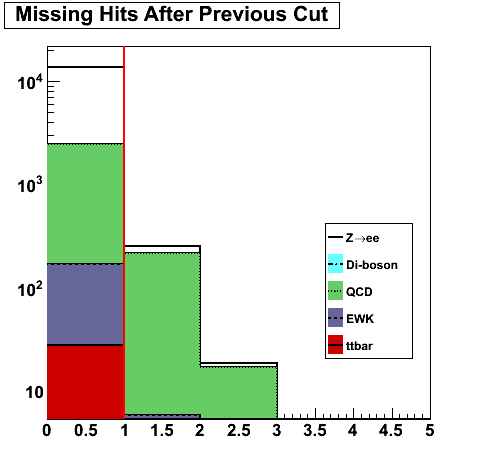
\includegraphics[width=180pt]{Figures/missHits-14Apr11.png}}
    \subfloat[$\Delta\cot\theta$]{\label{fig:DCotConvRejVars}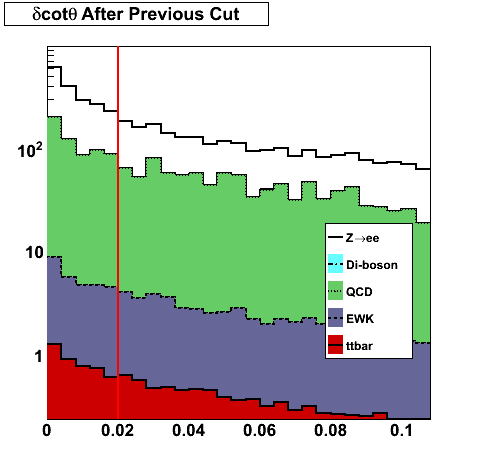
\includegraphics[width=180pt]{Figures/dCotTheta-14Apr11.png}}
    \subfloat[Dist]{\label{fig:DistConvRejVars}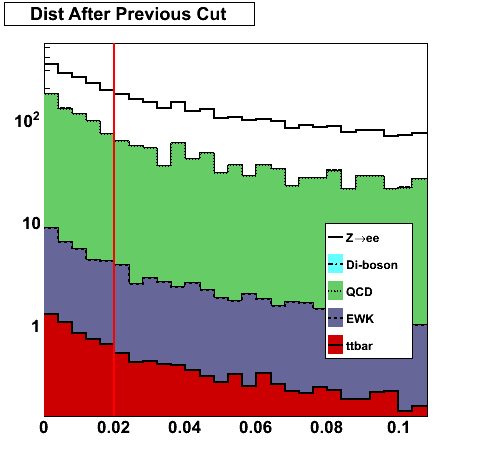
\includegraphics[width=180pt]{Figures/dist-14Apr11.png}}
  \end{center}
  \caption[Conversion rejection variables after previous cuts]{Conversion rejection variables after previous cuts.}
  \label{fig:ConvRejVars}
 \end{figure}


\subsubsection{Electron Isolation}
\label{evSel:isol}
It is expected that the products of a Z decay will not 
exit the interaction region  
in the vicinity of many other particles, 
since the Z decay products are not part of a jet.
We want to select those real electrons that are most likely to be prompt decay products,
not those that come from some secondary interaction with many other end products.  
Therefore we apply a set of cuts requiring little detector activity 
in the area immediately surrounding the reconstructed electron.  
The so-called isolation cuts look at the energy deposits 
in the electromagnetic and hadronic calorimeters separately,
as well as the total \pt of neighboring tracks, 
within specified \DR cones around the electron-associated deposit/track.  
These energies are divided by the \pt of the electron itself to arrive at a relative value,
which allows for higher-energy particles that may deposit more energy in the surrounding area.  
The thresholds for each of the three types of isolation is set separately for barrel and endcap, 
as given in Table \ref{TableEisoCuts}.  
Plots of the separate isolation distributions for both barrel and endcap 
are shown after previously-applied selection cuts in 
Fig.~\ref{fig:trkElecIsoVars} for track isolation, 
Fig.~\ref{fig:ecalElecIsoVars} for ECAL isolation, and 
Fig.~\ref{fig:hcalElecIsoVars} for HCAL isolation.  

%Conditions to require that electrons found are isolated, i.e. not contained in a jet with other particles.  
%We want (``prompt''?) electrons that come directly from the Z, 
%not from some other interaction with lots of other end products packaged along with the electron.  


%%%%  ISOLATION VALUES

\begin{table}[htbp]
%  \centering
  \begin{center}
    \caption{Thresholds for WP80 relative isolation.}
    \label{TableEisoCuts}
    \begin{tabular}[]{ | l | c | c | }
      \hline
      Cut variable & Barrel & Endcap  \\ \hline \hline
      Track & 0.09 & 0.04 \\ \hline
      ECAL & 0.07 & 0.05  \\ \hline
      HCAL & 0.10 & 0.025  \\ %\hline
%      $ H/E $ & 0.04 & 0.025  \\
      \hline
    \end{tabular}
  \end{center}
\end{table}


%%%% ISOLATION DISTROS

 \begin{figure}[htb]
  \begin{center}
    \subfloat[Barrel]{\label{fig:trkBarrelElecIsoVars}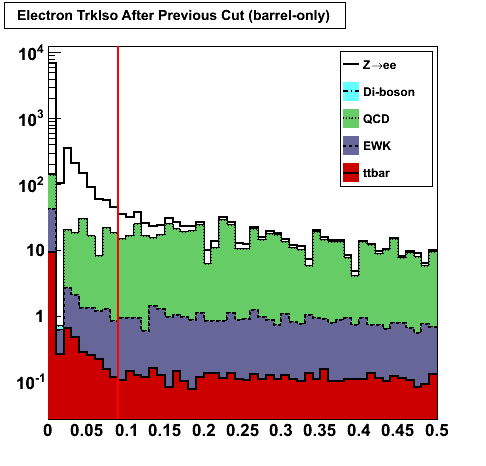
\includegraphics[width=180pt]{Figures/trkIso-barrel-14Apr11.png}}
    \subfloat[Endcap]{\label{fig:trkEndcapElecIsoVars}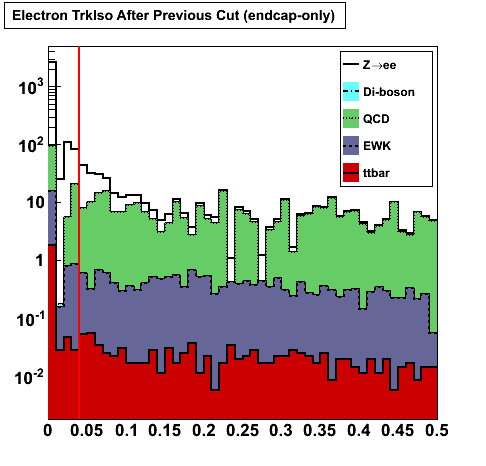
\includegraphics[width=180pt]{Figures/trkIso-endcap-14Apr11.png}}
  \end{center}
  \caption[Electron tracker isolation variables before respective cuts]{Electron tracker isolation variables before respective cuts.}
  \label{fig:trkElecIsoVars}
 \end{figure}



 \begin{figure}[htb]
  \begin{center}
    \subfloat[Barrel]{\label{fig:ecalBarrelElecIsoVars}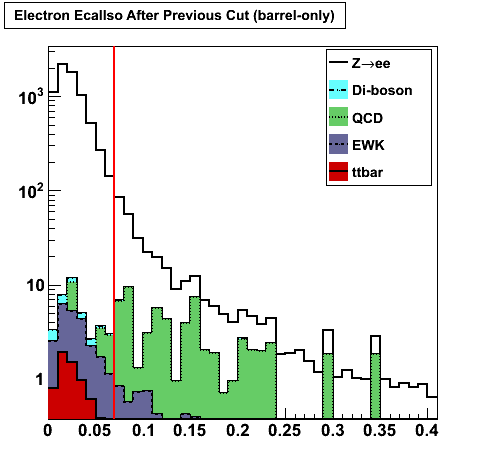
\includegraphics[width=180pt]{Figures/ecalIso-barrel-14Apr11.png}}
    \subfloat[Endcap]{\label{fig:ecalEndcapElecIsoVars}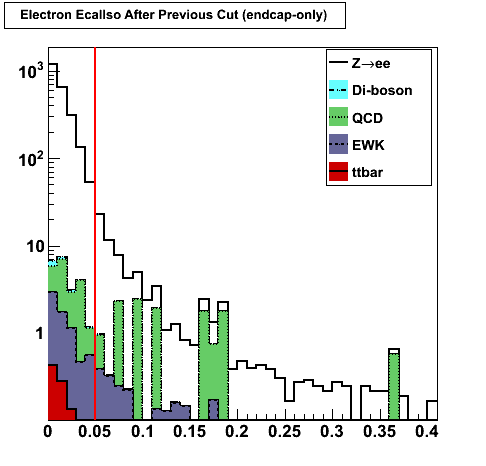
\includegraphics[width=180pt]{Figures/ecalIso-endcap-14Apr11.png}}
  \end{center}
  \caption[Electron ECAL isolation variables before respective cuts]{Electron ECAL isolation variables before respective cuts.}
  \label{fig:ecalElecIsoVars}
 \end{figure}



 \begin{figure}[htb]
  \begin{center}
    \subfloat[Barrel]{\label{fig:hcalBarrelElecIsoVars}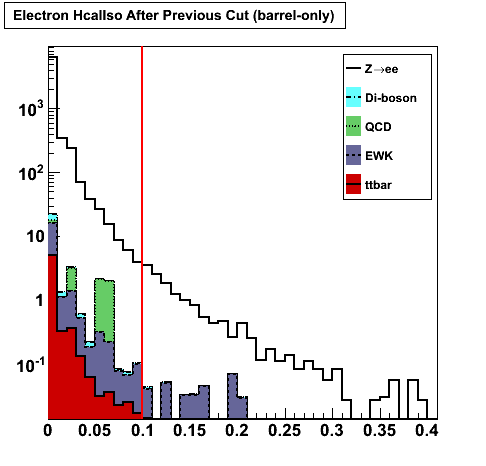
\includegraphics[width=180pt]{Figures/hcalIso-barrel-14Apr11.png}}
    \subfloat[Endcap]{\label{fig:hcalEndcapElecIsoVars}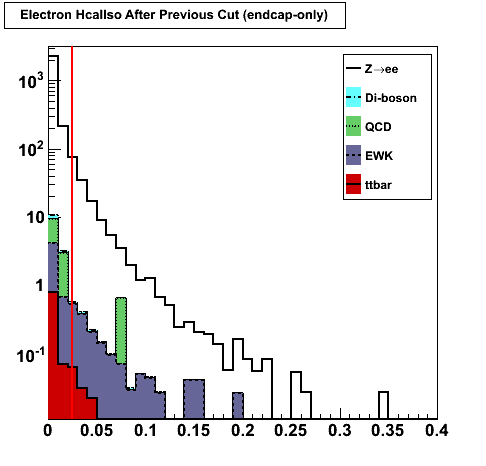
\includegraphics[width=180pt]{Figures/hcalIso-endcap-14Apr11.png}}
  \end{center}
  \caption[Electron HCAL isolation variables before respective cuts]{Electron HCAL isolation variables before respective cuts.}
  \label{fig:hcalElecIsoVars}
 \end{figure}



%Figures: Reconstructed electron/photon Pt, eta, phi spectra after isolation, Fig. \ref{fig:RecoSpectraAfterEidEiso}

% \begin{figure}[htb]
%  \begin{center}
%    
\includegraphics[width=80pt, angle=90]{CMS-BW.pdf}
%  \end{center}
%  \caption[Reconstructed electron/photon Pt, eta, phi spectra after isolation]{Reconstructed electron/photon Pt, eta, phi spectra after isolation.}
%  \label{fig:RecoSpectraAfterEidEiso}
% \end{figure}


\subsubsection{Electron Identification}
\label{evSel:eid}
Several ``electron identification'' variables are used to differentiate genuine electrons 
from other particles or conditions that may mimic electron behavior.  
Since an electron is reconstructed from a supercluster matched to a track, it is desired that the match is a good one.
The quality of matching can be estimated by looking at measures of the distance between the two components.
The position in $ \eta $ and $ \phi $ of the supercluster is compared with 
the $ \eta $ and $ \phi $ position of the track extrapolated back to the vertex, 
with the differences being labeled \detain and \dphiin, respectively.  
It is expected that a supercluster and track from the same electron will be close together, 
so upper limits on these quantities are defined as in Table \ref{TableEidCuts}.  
Distributions of electron \detain and \dphiin, 
each plotted after the previous selection step,% (conversion rejection),
are shown in Fig.~\ref{fig:dEtaInElecIdVars} and 
Fig.~\ref{fig:dPhiInElecIdVars}.  

The electron's energy deposit is also expected to be narrow relative to that of a jet.
A measure of the width in the $ \eta $ direction is therefore calculated 
using the energies and positions of the individual ECAL crystals, \sieie,
and this quantity is required to be below the thresholds listed in Table \ref{TableEidCuts}.  
(The $ \phi $ direction is not examined because bremsstrahlung from the electron 
can cause a significant spread of the energy in $ \phi $.)  
The \sieie distribution for electrons after all previous cuts is shown in 
Fig.~\ref{fig:sieieElecIdVars}.  
In addition, an electron is expected to deposit most of its energy in the 
electromagnetic portion of the calorimeter.  
A large hadronic energy deposit is more likely to come from a jet, 
so a limit on the ratio of the energy deposit in the electromagnetic calorimeter 
to that in the hadronic calorimeter, $ H/E $, is applied (values given in the table).  
The distribution of $H/E$ for electron candidates is plotted after 
all previous selection steps in Fig.~\ref{fig:hOeElecIdVars}.  


%%%% EID CUTS

\begin{table}[htbp]
%  \centering
  \begin{center}
    \caption{WP80 electron identification cuts.}
    \label{TableEidCuts}
    \begin{tabular}[]{ | l | c | c | }
      \hline
      Cut variable & Barrel & Endcap  \\ \hline \hline
      \sieie & 0.01 & 0.03  \\ \hline
      \dphiin & 0.06 & 0.03  \\ \hline
      \detain & 0.004 & 0.007 \\ \hline
      $ H/E $ & 0.04 & 0.025  \\
      \hline
    \end{tabular}
  \end{center}
\end{table}
%


%%%% EID DISTROS

\begin{figure}[htb]
  \centering
  %%  \begin{center}
  \subfloat[Barrel]{\label{fig:dEtaInBarrelElecIdVars}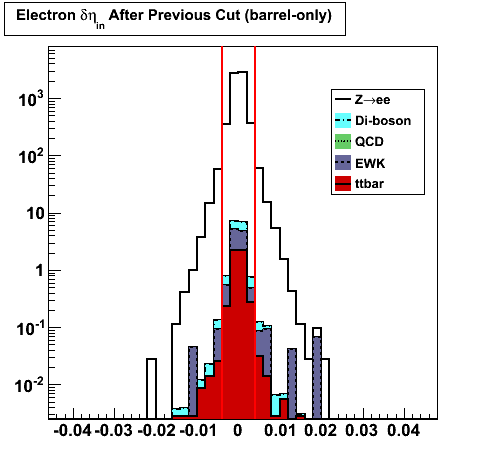
\includegraphics[width=180pt]{Figures/detain-barrel-14Apr11.png}}
  \subfloat[Endcap]{\label{fig:dEtaInEndcapElecIdVars}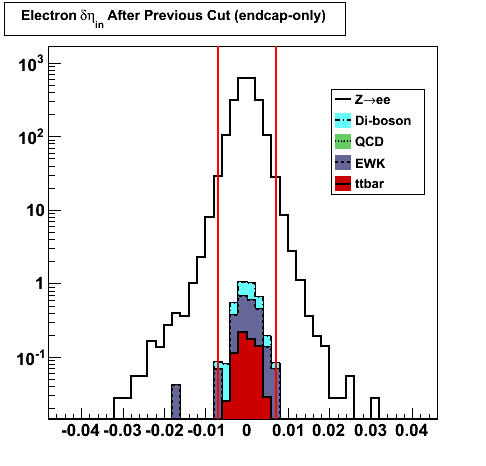
\includegraphics[width=180pt]{Figures/detain-endcap-14Apr11.png}}
  \caption[\detain electron identification variables after previous cuts]{
    \detain electron identification variables after previous cuts. 
    A low \detain indicates a good match between an electron candidate's 
    supercluster and track.  
    Values shown for \subref{fig:dEtaInBarrelElecIdVars} barrel and 
    \subref{fig:dEtaInEndcapElecIdVars} endcap.
  }
  \label{fig:dEtaInElecIdVars}
\end{figure}
  
  

 \begin{figure}[htb]
  \begin{center}
    \subfloat[Barrel]{\label{fig:dPhiInBarrelElecIdVars}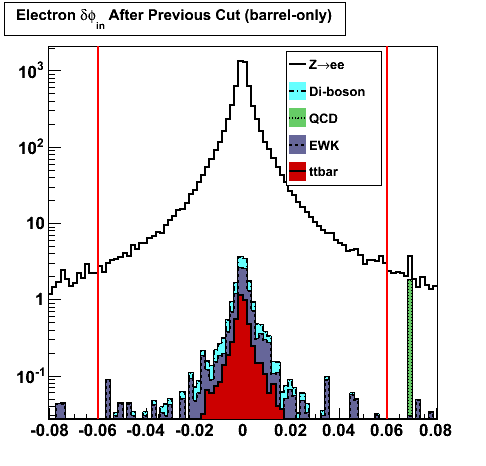
\includegraphics[width=180pt]{Figures/dphiin-barrel-14Apr11.png}}
    \subfloat[Endcap]{\label{fig:dPhiInEndcapElecIdVars}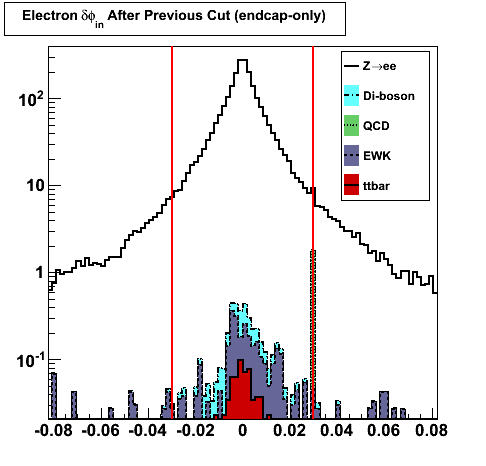
\includegraphics[width=180pt]{Figures/dphiin-endcap-14Apr11.png}}
  \end{center}
    \caption[\dphiin electron identification variables after previous cuts]{
      \dphiin electron identification variables after previous cuts.  
      A low \dphiin indicates a good match between the electron candidate's 
      supercluster and track.  
      Values shown for \subref{fig:dPhiInBarrelElecIdVars} barrel and 
      \subref{fig:dPhiInEndcapElecIdVars} endcap.
    }
  \label{fig:dPhiInElecIdVars}
 \end{figure}



 \begin{figure}[htb]
  \begin{center}
    \subfloat[Barrel]{\label{fig:sieieBarrelElecIdVars}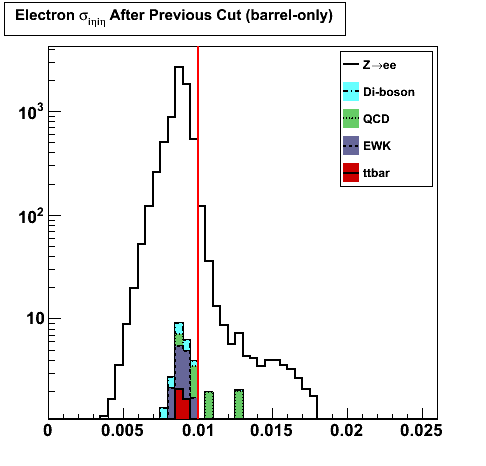
\includegraphics[width=180pt]{Figures/sieie-barrel-15Apr11.png}}
    \subfloat[Endcap]{\label{fig:sieieEndcapElecIdVars}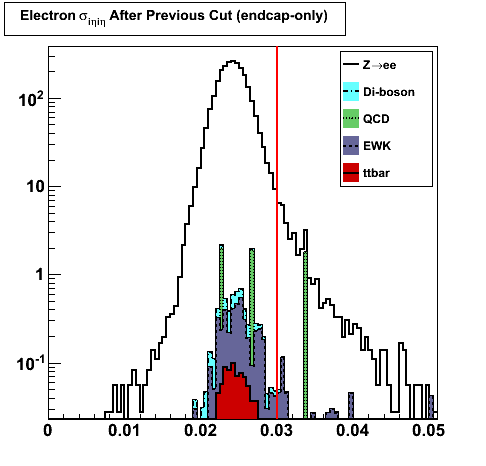
\includegraphics[width=180pt]{Figures/sieie-endcap-14Apr11.png}}
  \end{center}
    \caption[\sieie electron identification variables after previous cuts]{
      \sieie electron identification variables after previous cuts.  
      \sieie is a measure of the spread of the electron candidate's energy deposite in $\eta$.  
      A true electron is expected to be relatively narrow in $\eta$.  
      Values shown for \subref{fig:sieieBarrelElecIdVars} barrel and 
      \subref{fig:sieieEndcapElecIdVars} endcap.
    }
  \label{fig:sieieElecIdVars}
 \end{figure}



 \begin{figure}[htb]
  \begin{center}
    \subfloat[Barrel]{\label{fig:hOeBarrelElecIdVars}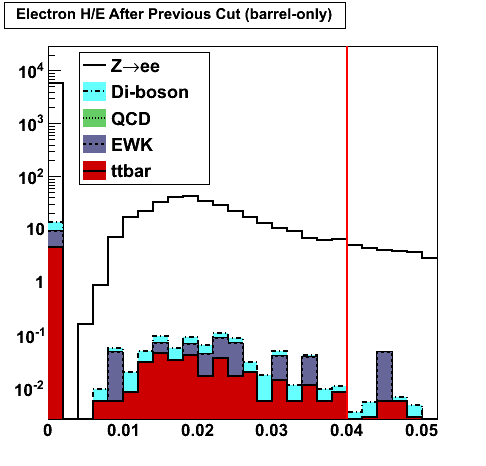
\includegraphics[width=180pt]{Figures/hoe-barrel-15Apr11.png}}
    \subfloat[Endcap]{\label{fig:hOeEndcapElecIdVars}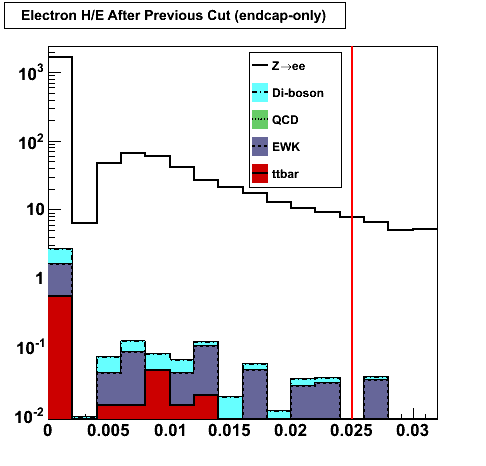
\includegraphics[width=180pt]{Figures/hoe-endcap-14Apr11.png}}
  \end{center}
    \caption[H/E electron identification variables after previous cuts]{
      H/E electron identification variables after previous cuts.  
      H/E is the ratio of the electron candidate's energy deposited 
      in HCAL to that deposited in ECAL.  
      A true electron is expected to deposit relatively little energy in the HCAL.  
      Values shown for \subref{fig:hOeBarrelElecIdVars} barrel and 
      \subref{fig:hOeEndcapElecIdVars} endcap.
    }
  \label{fig:hOeElecIdVars}
 \end{figure}



%Figures: Reconstructed electron/photon Pt, eta, phi spectra after ID, Fig. \ref{fig:RecoSpectraAfterEid}

 \begin{figure}[htb]
  \begin{center}
%    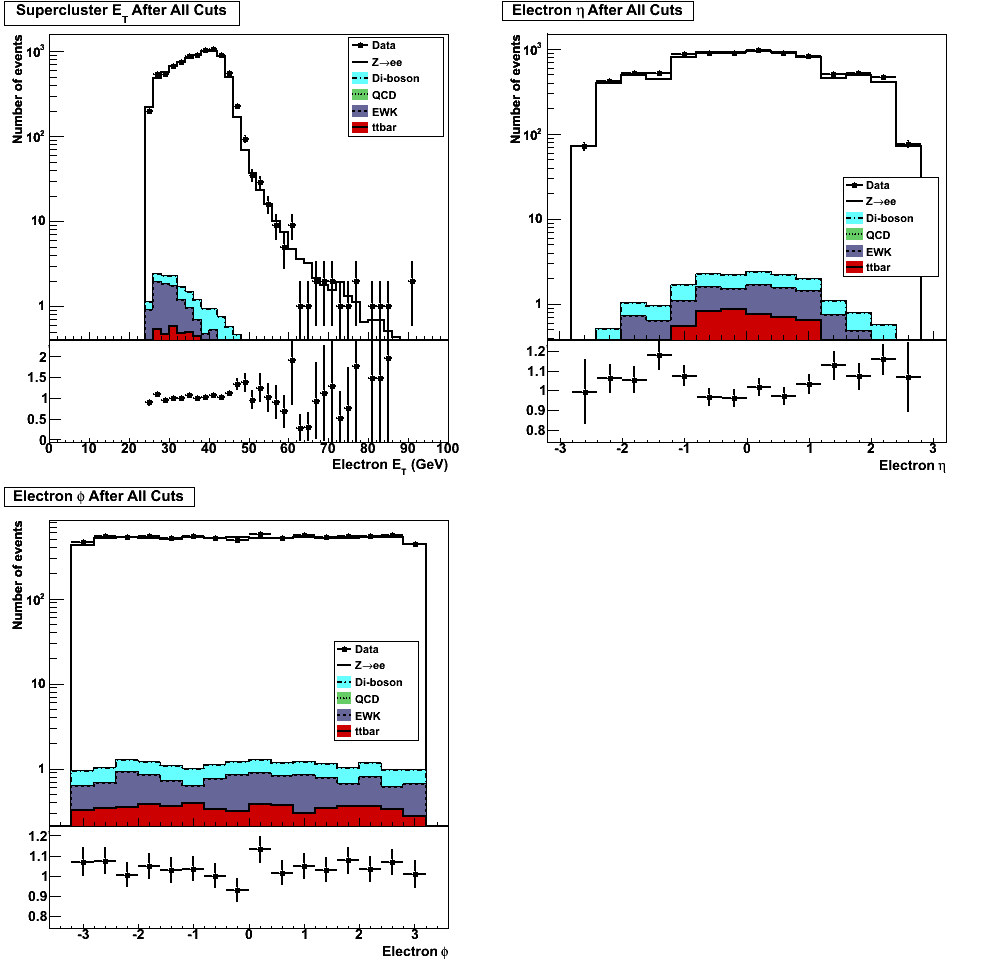
\includegraphics[width=180pt]{Figures/elecQuant-22Apr11.png}
%    \includegraphics[width=360pt]{Figures/elecQuant-22Apr11.png}
    \subfloat[Transverse Energy]{\label{fig:ElectronEtAfterCuts}\includegraphics[width=180pt]{Figures/elecScEt-18May11.png}}
    \subfloat[Pseudorapidity]{\label{fig:ElectronEtaAfterCuts}\includegraphics[width=180pt]{Figures/elecEta-18May11.png}}
    \subfloat[Azimuthal Angle]{\label{fig:ElectronPhiAfterCuts}\includegraphics[width=180pt]{Figures/elecPhi-18May11.png}}
  \end{center}
%  \caption[Reconstructed electron/photon Pt, eta, phi spectra after ID]{Reconstructed electron/photon Pt, eta, phi spectra after ID.}
   \caption[Reconstructed electron \pt, $\eta$, $\phi$ spectra after full selection]{
   Spectra of reconstructed electron kinematic quantities after all electron selection cuts. 
   The plots show distributions for electron \pt, $\eta$, and $\phi$ respectively.  
   The agreement between real data and the simulated sample is good, demonstrating 
   that the effects of the cuts on the data are understood.  
  }
  \label{fig:RecoSpectraAfterEid}
 \end{figure}


\subsubsection{Matching Offline-Reconstructed Objects to Trigger Objects}
\label{evSel:matching}
In order to ensure that the offline-reconstructed objects being examined were also reconstructed by the trigger, 
each offline object is compared with the list of trigger objects firing a given path.  %%% L1 also, or something?!
If the offline object lies close enough to a trigger object (measured by \DR{}), 
it is considered to have passed the trigger.  
%All electrons used in this analysis are required to be trigger-matched in this way.  
Each event in this analysis was required to have at least one electron trigger-matched in this way, 
within a \DR distance of 0.2.  
This demonstrates that the constituent objects in the event did in fact fire an appropriate trigger.  
%According to distribution of \DR between offline and trigger objects shown in Fig. \ref{fig:TriggerObjectSelectionDeltaR}, 
%the threshold was chosen to be NUMBER.

%Figures: \DR for L1 and HLT trigger object matching, Fig. \ref{fig:TriggerObjectSelectionDeltaR}

% \begin{figure}[htb]
%  \begin{center}
%    \includegraphics[width=360pt]{CMS-BW.pdf}
%  \end{center}
%  \caption[\DR for L1 and HLT trigger object matching to offline for electron selection]{\DR for L1 and HLT trigger object matching to offline-reconstructed objects.}
%  \label{fig:TriggerObjectSelectionDeltaR}
% \end{figure}


%\subsubsection{Electron Selection Performance} %wesley comment
%Figures: Reco PT resolution plots using MC reference for Z MC, Fig. \ref{fig:RecoPtResolution}

% \begin{figure}[htb]
%  \begin{center}
%    \includegraphics[width=80pt, angle=90]{CMS-BW.pdf}
%  \end{center}
%  \caption[Reco PT resolution plots using MC reference for Z MC]{Reco PT resolution plots using MC reference for Z MC.}
%  \label{fig:RecoPtResolution}
% \end{figure}


\subsection{\Zee Event Selection}
\label{evSel:zee}
%trigger (including list of good triggers), mass window... that might be all

In order to be included in the final selected sample of \Zee events, 
an event must have two electrons passing the selection cuts 
described in Section~\ref{evSel:elec}.  
Only one of the electrons is required to match to a trigger object, however; 
even if only one electron fires the trigger, 
the event is kept and the trigger's purpose is served, 
and there is no extra necessity for both electrons to fire the trigger.  
The two electrons are also required to have an invariant mass 
between 60 and 120 GeV; 
this defines a window around the Z mass peak at about 91 GeV.  
% TALK ABOUT INV MASS SOMEWHERE, PREV CH?

\subsubsection{Acceptance for \Zee Events}
\label{evSel:acc}
%full criteria, results
%discussion on acceptance: def, det acc vs ECAL acc, 
%systs due to theoretical vs other BUT PROB DON'T NEED SYSTS YET (do in separate ch)

% maybe end up putting def of acceptance in some more general place, like intro with that formula

The acceptance (abbreviated $A$) 
is the factor representing the fraction of events 
theoretically able to be detected with the given experiment.  
It includes considerations related to a particle's kinematic quantities 
(its position and momentum)
as well as to the precise definition of the signal interaction.  
In particular, the particle-detecting elements of any given 
detector, including CMS, do not fully cover the area around 
the interaction point -- 
by necessity, some of that area is taken up by the beam pipe.  
This means that any end-product particle that goes into a 
``dead'' space instead of a detecting element will not be 
detected.  
Therefore the acceptance factor takes into account the 
actual solid-angle area covered by the relevant parts of the detector.  
In addition, it is generally more difficult to distinguish 
very low-energy objects from background noise, 
so the acceptance also includes a lower limit on the 
energy of the particle.  
%It also must take into account the specific definition of the interaction.  
% 2 electrons w/in fiducial region, etc

In this analysis, the signal was defined to be those \Zee events 
whose invariant mass was between 60 and 120 GeV; 
this captures the Z peak around 90 GeV.  
The acceptance was defined as the fraction of those signal events 
whose electron end products fall into the $\eta$ region used for the 
analysis, 
%|eta| < 1.4442 || 1.5660 < |eta| < 2.4, %%%%%%%%%% FORMULIFY
$|\eta| < 1.4442$ or $1.566 < |\eta| < 2.5$,
and whose transverse energies were both above 25 GeV.  
These values can also be found in Table~\ref{TableAccCuts}.  

%Make table with those criteria 

\begin{table}[htbp]
%  \centering
  \begin{center}
    \caption{Criteria for determining acceptance.}
    \label{TableAccCuts}
    \begin{tabular}[]{ | l | c | }
      \hline
      Kinematic quantity & Requirement  \\ \hline \hline
      $\eta$ & $|\eta| < 1.4442$ or $1.566 < |\eta| < 2.5$  \\ \hline
      \Et & $ < 25 GeV$  \\ 
      \hline
    \end{tabular}
  \end{center}
\end{table}


%determined by MC estimates; room for theoretical uncertainties

Acceptance cannot be calculated from data, 
because it is impossible to know how many events were missed -- 
the only events we have are those which were not missed.  
Instead acceptance is determined by applying the defining 
criteria to a sample of simulated data, 
a sample large enough that statistical uncertainties become 
small enough to ignore.  
Since the simulated sample is expected to model real data well enough, 
this number is taken as the true acceptance for real data.  
However, the information used to generate the simulated sample 
is only a theoretical model; 
there are many ways in which it may actually differ slightly from 
what is used in the generation.  
These possible differences are taken into account in the 
uncertainty calculated for the acceptance, 
% OR JUST DO IT HERE??????
which will be detailed in a later section.  %FIXME add section number

It is also useful to combine the 
supercluster reconstruction efficiency with the acceptance. 
The supercluster reconstruction efficiency is impossible 
to determine from data for the same reason as for 
the acceptance -- 
it would require knowing about 
events that were missed, in this case 
electrons that had impacted the detector 
(specifically ECAL) but which had 
not resulted in the formation of a supercluster.  
% what about test-beam data??  I guess doesn't 
% take into account brem or pileup or non-isolation 
% or any of that stuff that could affect it
Therefore this is also determined from simulated data.  
Effectively it is combined with the acceptance 
by applying an additional requirement on the acceptance: 
the simulated event should have two electrons 
passing the $\eta$ and transverse energy requirements, 
and those electrons should also both be matched 
to reconstructed superclusters.  
The fraction of total events passing these combined criteria 
is referred to as 
``ECAL acceptance'' or $A_{ECAL}$.  

The pure kinematic acceptance for this analysis
was determined 
with the POWHEG-generated Monte Carlo sample 
to be 
\AVal{} %0.423 %BLAH1
and the ECAL acceptance was likewise calculated as 
\AEcalVal. %0.387. %BLAH2.  
These values can also be found in Table~\ref{TableAccValues}.  


%also make table with calculated values

\begin{table}[htbp]
%  \centering
  \begin{center}
    \caption{Acceptance values.}
    \label{TableAccValues}
    \begin{tabular}[]{ | l | c | c | }
      \hline
      Quantity & Value  \\ \hline \hline
      $ A $ & \AVal  \\ \hline
      $ A_{ECAL} $ & \AEcalVal  \\
      \hline
    \end{tabular}
  \end{center}
\end{table}



% MAYBE ALSO PUT THIS SECTION SOMEWHERE ELSE, even the results part

% PREV CH: DEFINE SIGNAL, BACKGROUND.  MAYBE HAVE A GLOSSARY???

\subsubsection{Efficiency of Selection for \Zee Events}
\label{evSel:eff}
%Def of efficiency (you have to know about events that were missed, could put before acc if necessary but might not be necessary...); 
%talk about different steps; 
%trigger effs done here or in trigger section (maybe easier here, because introduce T\&P here)

It is important to know how well the selection steps perform their task of 
keeping signal events;  
any signal events that are 
missed %cut out 
must be accounted for in the final 
calculation to get an accurate result.  
This factor is quantified in the efficiency, which is defined as 
the fraction of total objects or events passing a given selection. % is called 
%the selection efficiency.% and is used to 
Simulated data can be used to calculate efficiency, 
since it contains the ``truth'' information -- 
the true total number of events, 
whether or not they survive a given selection step.
However, the simulation may not correctly model some 
aspect of the real data, which would cause a discrepancy 
with the real-data efficiency 
and a corresponding inaccuracy in the final result.  
Therefore it is desirable to use so-called ``data-driven'' 
methods, % of determining efficiency, 
determining the efficiency as closely as possible 
using only the data itself.  
Because the truth information does not exist in real data, 
%another way must be used to determine how many 
the number of events passing or failing a given selection 
must be determined with another method.  

%Tag and Probe:  
The tag-and-probe method is used to determine the efficiency of a given set of electron selection steps.  
In this method, a set of data events is identified which appear to be good 
%Z->ee 
\Zee
candidate events.  
One of the electrons in each of these events must pass 
all selection cuts and essentially be identified as a golden electron; 
%some stringent
this is the tag.  
%The other electron must 
%pass some less stringent criteria
%be identified at least as a supercluster; 
The criteria applied to the other electron are looser: 
it is not required to pass the selection cuts being tested.  
This is the probe electron.  
The event's status as a Z candidate is determined by enforcing 
a mass window cut on the invariant mass of the tag-probe system 
(this is sufficient %(enough?) 
to select a high-purity sample of 
events in which both legs are real electrons).
% -- REFERENCE??).  
The naive selection efficiency is then given by the fraction 
of probe electrons that pass the requirement being tested.  

However, a more sophisticated analysis of the efficiency can 
be performed by fitting the invariant mass spectra of the
tag-probe pairs for both passing and failing probes to a 
lineshape representing both the signal and the background.  
Then the distribution of passing probes can be represented as 
the signal lineshape multiplied by the efficiency and the
total number of signal events added to the background lineshape 
multiplied by the number of passing background events.  
The failing probe distribution can be represented in the 
analogous way, using (1 - efficiency) instead.  
From this pair of fits the total number of events as well as 
the efficiency can be extracted simultaneously.  

However, the tag-and-probe may possibly introduce a bias 
into the calculation, 
in particular if observing one leg makes it more likely that 
the other leg is observed. 
For example, if the electrons are essentially back-to-back, 
one is more likely to fall within the detector coverage 
if the other one does as well.  
In addition, there is a slight discrepancy between the efficiencies 
calculated using data and those using the standard Monte Carlo sample.  
Therefore, the strategy in this analysis is to calculate the 
``true'' efficiency from the simulation sample, 
as well as the tag-and-probe efficiencies from the real data 
and simulation samples.  
The ``true'' efficiency is then corrected by the ratio of the 
data and simulation tag-and-probe efficiencies:
\[
\epsilon = \epsilon_{MC}^{true} \times \left( \frac{\epsilon_{data}^{T\&P}}{\epsilon_{MC}^{T\&P}} \right)
\]
This implies a certain amount of trust in the generator-level simulation of the interaction.  
The corresponding uncertainty in the efficiency due to the generator-level simulation 
is dealt with in a later chapter.  %FIXME say which

The event selection efficiency in this analysis is determined 
by first obtaining the efficiencies of the individual 
selection steps given above.%, using the tag-and-probe method.  
This also includes the initial step of reconstructing 
the electron objects from superclusters.  
Since each selection step is applied one after the other, 
the overall selection efficiency is given by the product 
of the individual efficiencies.  
In addition, since most steps are required to apply to both electrons, 
the single-electron efficiencies of these steps 
(the result of the tag-and-probe method)
are squared to get 
the efficiency of both electrons passing that step.  
The trigger step, however, is a special case since only one electron is 
required to pass.  
In this case, the quantity used is the probability that at least 
one electron passes, 
which is equivalent to the probability both electrons fail 
subtracted from 1.  

% cute little genetics probability diagram illustration??  I kind of like that idea

The formula used to calculate the overall event selection efficiency 
from the individual step efficiencies is therefore 
\[
%BIG FAT FORMULA
\epsilon_{total} = \epsilon_{reco}^2 \times \epsilon_{isol}^2 \times \epsilon_{ID}^2 \times \left( 1 - \left( 1 - \epsilon_{trig} \right)^2 \right)
\]

%explain MC truth vs MC T\&P vs data T\&P (plot illustrating problem??  not really, I guess)




The efficiencies are given for each selection step in Table~\ref{TableEfficiencies} %.   %FIXME ALSO DO FOR BARREL/ENDCAP
and for all the triggers used in data individually in Table~\ref{TableTriggerEfficiencies}.  

\begin{table}[htbp]
  \begin{center}
    \caption{Efficiencies of electron selection steps.}
    \label{TableEfficiencies}
    \begin{tabular}[]{ | l | l | l | l | l | l | }
      \hline
%      STUFF \\ \hline
      Step & True MC & MC T\&P & Data T\&P & Ratio & Efficiency \\ \hline \hline
      %SC to Gsf & 0.965 & 0.972 & 0.971 +/- 0.002 & 0.999 +/- 0.002 & 0.964 +/- 0.002 \\ \hline
      Reconstruction & 0.965 & 0.972 & 0.971 +/- 0.002 & 0.999 +/- 0.002 & 0.964 +/- 0.002 \\ \hline
      %Gsf to Iso & 0.926 & 0.927 & 0.910 +/- 0.003 & 0.976 +/- 0.003 & 0.905 +/- 0.003 \\ \hline
      Isolation & 0.926 & 0.927 & 0.910 +/- 0.003 & 0.976 +/- 0.003 & 0.905 +/- 0.003 \\ \hline
      %Iso to Id & 0.906 & 0.907 & 0.897 +/- 0.003 & 0.989 +/- 0.003 & 0.896 +/- 0.003 \\ \hline
      Identification & 0.906 & 0.907 & 0.897 +/- 0.003 & 0.989 +/- 0.003 & 0.896 +/- 0.003 \\ \hline
      %Id to HLT & 0.959 & 0.941 & 0.972 +/- 0.001 & 1.032 +/- 0.001 & 0.991 +/- 0.001 \\ \hline
      Trigger & 0.959 & 0.941 & 0.972 +/- 0.001 & 1.032 +/- 0.001 & 0.991 +/- 0.001 \\ \hline
      Full Event selection & 0.654 & 0.665 & 0.621 +/- 0.005 & 0.933 +/- 0.007 & 0.610 +/- 0.005 \\ \hline
    \end{tabular}
  \end{center}
\end{table}


%Figures: Efficiency table and supporting plots

%   * tag and probe fit plots (most in an appendix, I'd say) %FIXME

%   * BIG GIANT EFFICIENCY TABLES for each step/barrelvsendcap/datavsMC(/differentMCsamples?NO)

%   * do trigger effs separately, I guess!  Under trigger section.  or just put table here

\begin{table}[htbp]
  \begin{center}
    \caption[Efficiencies of data trigger paths]{Efficiencies of all the triggers used in data as determined with the tag-and-probe method.}
    \label{TableTriggerEfficiencies}
    \begin{tabular}[]{ | l | l | l | }
      \hline
      Trigger	& Efficiency & Error (fit) \\ \hline \hline
      HLT\_Photon15\_Cleaned\_L1R & 0.976 & 0.002 \\ \hline
      HLT\_Ele15\_LW\_L1R & 0.961 & 0.005 \\ \hline
      HLT\_Ele15\_SW\_L1R & 0.981 & 0.003 \\ \hline
      HLT\_Ele15\_SW\_CaloEleId\_L1R & 0.986 & 0.003 \\ \hline
      HLT\_Ele17\_SW\_CaloEleId\_L1R & 0.992 & 0.002 \\ \hline
      HLT\_Ele17\_SW\_TightEleId\_L1R & 0.973 & 0.002 \\ \hline
      HLT\_Ele17\_SW\_TighterEleIdIsol\_L1R\_v1 & 0.973 & 0.003 \\ \hline
      HLT\_Ele17\_SW\_TighterEleIdIsol\_L1R\_v2 & 0.977 & 0.002 \\ \hline
      HLT\_Ele17\_SW\_TighterEleIdIsol\_L1R\_v3 & 0.974 & 0.003 \\ \hline
      Overall & 0.9763 & 0.0009 \\ \hline
    \end{tabular}
  \end{center}
\end{table}

\subsubsection{Distribution of Z Kinematic Variables}
\label{evSel:Zquants}
%Some amount of text explaining what this is for!  
Since a significant number of \Zee candidate events have been identified, 
it is useful to examine the kinematic properties of these events.  
Even though this analysis does not depend on these properties, 
comparing the distributions from the data with those from the simulated samples 
can provide an additional check of validity of the simulation.  

Fig. \ref{fig:Zquantities} shows the distributions of standard kinematic 
variables for the reconstructed Z candidates: transverse momentum, rapidity, and azimuthal angle. 
The data (black dots) is compared with the simulation including 
background samples (lines/filled areas).  
As the ratio plots show, the agreement is good in general; 
large error bars indicate bins where the event count is not 
high enough to give a very precise estimate 
(such as the higher range of the Z \pt plot).  
However, there are areas in which there is an evident discrepancy 
between the data and the simulation, 
most notably along the outer edges of the Z rapidity plot.  
Possible causes might include a slightly inaccurate description of the particle 
interaction in the generator, 
or a slight miscalibration of the detector.  
Since the difference is slight and does not affect this analysis, though, 
it can safely be ignored and the general agreement accepted.  

%Dude, what else to say here?  

 \begin{figure}[htb]
  \begin{center}
%    \includegraphics[width=360pt]{Figures/Zquantities-04Apr11.png}
    \subfloat[Transverse Momentum]{\label{fig:ZPt}\includegraphics[width=180pt]{Figures/Zpt-18May11.png}}
    \subfloat[Rapidity]{\label{fig:ZRap}\includegraphics[width=180pt]{Figures/Zrap-18May11.png}}
    \subfloat[Azimuthal Angle]{\label{fig:ZPhi}\includegraphics[width=180pt]{Figures/Zphi-18May11.png}}
  \end{center}
  \caption[Kinematic quantities of Z candidates after full selection]{
  Kinematic quantities of Z candidates after full event selection.
  }
  \label{fig:Zquantities}
 \end{figure}



\clearpage

\newcommand{\nevents}{8453}

\chapter{Analysis Method}
\label{anMeth}
I guess this is the part of the analysis that's not included in event selection.  
SO, how to get the cross section, like the main formula, 
and where all the numbers came from (especially the ones we haven't calculated yet).

%recap of invariant mass?

\section{This all should have its own section}

As explained in Section FIXME, 
the invariant mass of a set of decay-product particles is 
%CONCEPTUAL EXPLANATION.
essentially the mass of the original particle that decayed. 
%to form the end-products.  
It is defined mathematically as 

INV MASS FORMULA

where p momentum, E energy, etc. 
In our case, for a two-particle system, it can be written as 

MORE FORMULA (this one necessary??)

The invariant mass distribution for the electron pairs 
in the events surviving all selection cuts is shown in 
Fig.~\ref{fig:InvMass}.  
The peak around the Z mass (\~91 GeV) is clearly visible 
in both the Monte Carlo and data distributions.  

%yield plot first, since this is what the rest is based on.  

%%Figures: Electron-pair invariant mass for trigger objects/ID only/ID+isolation, Fig. \ref{fig:InvMassAfterEachStep}
%Figures: Electron-pair invariant mass after full selection, Fig. \ref{fig:InvMass}

 \begin{figure}[htb]
  \begin{center}
    \includegraphics[width=360pt]{Figures/invMass-04Apr11.png}
  \end{center}
  \caption[Electron-pair invariant mass after full selection]{Electron-pair invariant mass after full selection.}
  \label{fig:InvMass}
 \end{figure}

% Also add plots for OS and SS??  Had them at one point!  
% WELL, last OS plot I have does not show good data/MC agreement

%% Figures: Same-sign dielectron invariant mass for electrons passing all selection steps, Fig. \ref{fig:SameSignInvMass}

%%  \begin{figure}[htb]
%%   \begin{center}
%%     \includegraphics[width=360pt]{CMS-BW.pdf}
%%   \end{center}
%%   \caption[Same-sign dielectron invariant mass for electrons passing all selection steps]{Same-sign dielectron invariant mass for electrons passing all selection steps.}
%%   \label{fig:SameSignInvMass}
%%  \end{figure}

Ooh, I do also have inv mass by eta plots

 \begin{figure}[htb]
  \begin{center}
%    \includegraphics[width=360pt]{Figures/invMass-04Apr11.png}
    \subfloat[Barrel-barrel]{\label{fig:InvMassEtaDivBarrelBarrel}\includegraphics[width=180pt]{Figures/invMassEtaDiv-barrel-barrel-19May11.png}}
    \subfloat[Barrel-endcap]{\label{fig:InvMassEtaDivBarrelEndcap}\includegraphics[width=180pt]{Figures/invMassEtaDiv-barrel-endcap-19May11.png}}
    \subfloat[Endcap-endcap]{\label{fig:InvMassEtaDivEndcapEndcap}\includegraphics[width=180pt]{Figures/invMassEtaDiv-endcap-endcap-19May11.png}}
  \end{center}
  \caption[Electron-pair invariant mass by $\eta$]{
    Electron-pair invariant mass by $\eta$ after full selection.
    Each combination of electron $\eta$-positions is 
    distributed separately: 
    both electrons in the barrel 
    %(Fig.~\ref{fig:InvMassEtaDivBarrelBarrel}), 
    \subref{fig:InvMassEtaDivBarrelBarrel}, 
    one electron each in the barrel and the endcap 
    %(Fig.~\ref{fig:InvMassEtaDivBarrelEndcap}),
    \subref{fig:InvMassEtaDivBarrelEndcap},
    and both electrons in the endcap 
    %(Fig.~\ref{fig:InvMassEtaDivEndcapEndcap}).
    \subref{fig:InvMassEtaDivEndcapEndcap}.
    In each case the agreement between data and Monte Carlo simulation is good.  
  }
  \label{fig:InvMassEtaDiv}
 \end{figure}

The total number of data events surviving 
the selection cuts is \nevents{}. %8453.  
% mention slight upward shift in data of peak position here?

ALSO TALK ABOUT HOW PLOTS SCALED??!!  somewhere, like in event selection?


The formula to calculate the cross section from Section FIXME is

FORMULA

where the terms refer to blah blah blah.  
Essentially it means that. %FIXME
Most of the required numbers have been dealt with 
in other chapters.  % remove?

Explain formula in detail here?  
It really is the analysis method.  
You plug in the numbers and get the cross section.  
Some of the pieces have been done in other 
chapters, like acceptance and efficiency 
(ntotal is done above, I guess, just from 
looking at inv mass plot which isn't strictly 
necessary, either!)  
Should they instead all be done here?  

recap of formula:

THE FORMULA

   * ntotal
   * nbg -- THE DIFFERENT METHODS OF BACKGROUND SUBTRACTION
   * acc (event sel)
   * eff (event sel) -- but talk about correcting for data/MC difference
   * Lumi (exp chapter or sth)

ntotal comes from inv mass plot just shown, nbg is what you need to calculate.
3 methods: 
   * MC estimate
   * template method
   * sideband subtraction

You know, I don't think my analysis needs a whole giant section on data vs MC comparison.  
I didn't do a whole lot on that.  
Well, just write up what I did do, I guess.  

%\section{Comparison of Monte Carlo and Data}
\section{Background Subtraction}
\label{anMeth:BGSub}
It is expected that some number of non-signal events %, 
%or background events, 
will look enough like signal events to pass the full selection.  
These background events need to be accounted for 
in the final calculation to arrive 
at the most accurate result.  
Therefore, the number of background events should 
be estimated and subtracted from the total number 
of events; 
This estimation can be done in a variety of ways.  
The methods used in this analysis are detailed 
in the following sections.  

Figures: Background subtracted yield versus eta with a MZ mass window - comparison to MC, Fig. \ref{fig:YieldVsZEtaComparedToMC}

 \begin{figure}[htb]
  \begin{center}
    \includegraphics[width=360pt]{CMS-BW.pdf}
  \end{center}
  \caption[Background subtracted yield versus eta with a MZ mass window - comparison to MC]{Background subtracted yield versus eta with a MZ mass window - comparison to MC.}
  \label{fig:YieldVsZEtaComparedToMC}
 \end{figure}

Figures: Background subtracted Z PT distribution with a MZ mass window - comparison to MC, Fig. \ref{fig:YieldVsZPtComparedToMC}

 \begin{figure}[htb]
  \begin{center}
    \includegraphics[width=360pt]{CMS-BW.pdf}
  \end{center}
  \caption[Background subtracted Z PT distribution with a MZ mass window - comparison to MC]{Background subtracted Z PT distribution with a MZ mass window - comparison to MC.}
  \label{fig:YieldVsZPtComparedToMC}
 \end{figure}

\subsection{Monte Carlo Estimation}
\label{anMeth:BGSubMC}
One estimate of the number of background events can be made 
directly from the Monte Carlo simulation, 
by counting the number of simulated events that pass 
the full selection.  
The numbers of passing events for the simulated background 
samples used are shown in Table~\ref{TableBackgroundMC}, 
with a total of 18.5 events.  
The accuracy of this method may be questionable due to 
unaccounted differences between the simulation and real data, however.  
In particular, 
the detector may not be correctly modeled in the simulation, 
causing slight differences in event numbers 
that are non-negligible at this level.  
Therefore, data-driven methods of background subtraction 
are also used, 
and the results from all the methods are checked against each other 
to confirm the accuracy of each method.  

%TABLE with MC-estimated number of events from each background source

\begin{table}[htbp]
%  \centering
  \begin{center}
    \caption{Number of events passing full selection 
      for each background, estimated from 
      Monte Carlo simulation.}
    \label{TableBackgroundMC}
%    \begin{tabular}[]{ | l | c | c | }
    \begin{tabular}[]{ | l | c | }
      \hline
      Background Sample & Number of Events  \\ \hline \hline
      Wenu & 0.36 \\ \hline % 0.35799
      Wtaunu & 0 \\ \hline % 0
      Ztautau & 6.4 \\ \hline % 6.3777
      Electroweak Total & 6.7 \\ \hline \hline % 6.73569
      ttbar & 5.8 \\ \hline \hline % 5.83397
      QCD & 0. \\ \hline \hline % Hah
      WW & 1.5 \\ \hline % 1.5382
      WZ & 1.4 \\ \hline % 1.4396
      ZZ & 3.0 \\ \hline % 2.9984
      Di-boson Total & 6.0 \\ \hline \hline % 5.9762
      Total Background & 18.5 \\ \hline % 18.54586
    \end{tabular}
  \end{center}
\end{table}



\subsection{Template Method}
\label{anMeth:BGSubTemplate}
The template method is a data-driven method 
to estimate the background contribution 
in a selected sample.  
In general, it uses modified cuts 
to select data events that are especially 
likely to be signal or background; 
these subsamples are called templates.  
Extra-tight cuts select a ``signal-rich'' sample, 
while a combination of loose and inverted cuts 
select a ``background-rich'' sample.  
A particular selection variable is chosen 
which has significantly different distributions 
for signal and background; 
here, the relative tracker isolation variable is used.  
The template method compares the 
distributions of that variable 
from the selected signal and background templates 
to the distribution from the full data sample. %, 
Essentially, the method determines what 
combination of the signal and background templates 
best fits the data distribution, 
in an effort to determine what fraction 
of the data sample is signal 
and what fraction is background.  
This method is only useful to determine the 
background from QCD; 
its technique relies on ``background'' electrons 
being qualitatively different from 
``good electrons'' 
(measured by the variable being used), 
but electrons from interactions similar 
to the signal interaction, 
such as \Wenu, 
are also ``good electrons.''  
Objects arising from QCD interactions that are 
identified as ``electrons'' are more likely 
clusters of hadronic particles 
that come out looking like electrons, 
so they can be distinguished from 
``good electrons'' and therefore 
%used in this method.  
%used for this method.  
the template method can identify 
them as background.  

\subsubsection{Template Definitions}
\label{anMeth:BGSubTemplateDefs}
%defs of tighter and looser selections (bleah), more tables?

Several new working points, based on WP80 
(defined in Section~\ref{evSel:elec}), were defined to select 
the signal-like and background-like template samples, 
as well as the data distribution used in the comparison.  

The first working point, used to select the data, 
is called ``Semi-Tight'' and is identical to WP80 
except for the removal of its relative track isolation 
requirement.  
This is solely to allow the full spectrum of track 
isolation values to be examined.   
All events with two electrons passing the 
Semi-Tight working point are 
included in the data sample.  

The working point used to select the ``signal-rich'' 
data sample is called ``Tight'' 
and is based on the Semi-Tight working point 
but with a few cuts made tighter.  
(This is to ensure a very pure sample; 
however, a very tight working point would not work 
for standard data selection because its 
efficiency is lower -- 
it cuts out too many good events.  
For the template method, though, a lower number 
of events is sufficient.)  
The tighter cut values were taken from WP70, 
another of the standard working points. %, 
%and the modified values are given in Table~\ref{TableWPs}.  
%In particular, 
Specifically, 
the values for 
\dphiin in both the barrel and the endcap, 
$H/E$ in the barrel, 
and \detain in the endcap 
were modified.  
To select the signal template sample, 
each event was required to have two electrons 
passing the Tight working point, 
and the two electrons were required to have 
opposite signs.  

The final working point used for the template method 
is the ``Loose'' working point, 
which is used in selecting the background template.  
The Loose working point is modeled on the 
Semi-Tight working point, as is the Tight, 
but for the Loose working point 
all the thresholds for the isolation 
and electron isolation variables 
are increased by a factor of 5.  
In addition, in order to get enough data 
for a reasonable background template, 
the ECAL isolation variable had to be further loosened, 
from 0.07 to 2.5 in the barrel and from 0.05 to 1.0 in the endcap, 
and the supercluster \Et cut had to be lowered 
from 25 GeV to 20 GeV.  
Events selected for the background template 
must have two electrons, 
one passing the Semi-Tight working point 
and one passing the Loose, 
and these two electrons are required to 
have the same sign in order to reject signal.  

%HOW TO DO TABLES: just one giant table showing all WP's?  
%highlight changed values?  HA, with italics
%(or tables of just changed values?)

Table~\ref{TableWPs} shows the cut values for 
WP80 and how each of the working points used 
in the template method is modified with 
respect to WP80.  
Cut values changed with respect to WP80 
are displayed in italics.  


% WP'S
\begin{table}[htbp]
%  \centering
  \begin{center}
    \caption{
      Summary of the standard working point as well as 
      the working point definitions used 
      in the template method.
      Italics indicates a cut changed relative to WP80.
    }
    \label{TableWPs}
%    \begin{tabular}[]{ | l | c | c | }
    \begin{tabular}[]{ | l | c | c | c | c | c | c | c | c | }
      \hline
      Cut Variable & \multicolumn{2}{|c|}{WP80} & \multicolumn{2}{|c|}{Semi-Tight} & \multicolumn{2}{|c|}{Tight} & \multicolumn{2}{|c|}{Loose}  \\ \hline \hline
      & Barrel & Endcap & Barrel & Endcap & Barrel & Endcap & Barrel & Endcap \\ \hline
%      Conversion Rejection    & & & & & & & &  \\ \hline % 
      \multicolumn{9}{|l|}{Conversion Rejection}   \\ \hline % 
      missing hits            & 0    & 0    & 0    & 0    & 0    & 0    & 0    & 0     \\ \hline % 
      dist                    & 0.02 & 0.02 & 0.02 & 0.02 & 0.02 & 0.02 & 0.02 & 0.02  \\ \hline % 
      $\delta\cot\theta$      & 0.02 & 0.02 & 0.02 & 0.02 & 0.02 & 0.02 & 0.02 & 0.02  \\ \hline % 
%      Relative Isolation & & & & & & & &  \\ \hline % 
      \multicolumn{9}{|l|}{Relative Isolation}   \\ \hline % 
      ECAL      & 0.07 & 0.05 & 0.07 & 0.05 & 0.07 & 0.05 & \textit{2.5} & \textit{1.0}  \\ \hline % 
      HCAL      & 0.1 & 0.025 & 0.1 & 0.025 & 0.1 & 0.025 & \textit{0.5} & \textit{0.125}  \\ \hline % 
      track     & 0.09 & 0.04 & \textit{N/A} & \textit{N/A} & \textit{N/A} & \textit{N/A} & \textit{N/A} & \textit{N/A}  \\ \hline % 
%      Electron Identification & & & & & & & &  \\ \hline % 
      \multicolumn{9}{|l|}{Electron Identification}   \\ \hline % 
      \sieie          & 0.01  & 0.03  & 0.01  & 0.03  & 0.01  & 0.03  & \textit{0.05} & \textit{0.15}  \\ \hline % 
      \dphiin         & 0.06  & 0.03  & 0.06  & 0.03  & \textit{0.03} & \textit{0.02} & \textit{0.3} & \textit{0.15}  \\ \hline % 
      \detain         & 0.004 & 0.007 & 0.004 & 0.007 & 0.004 & \textit{0.005} & \textit{0.02} & \textit{0.035}  \\ \hline % 
      $H/E$           & 0.04  & 0.025 & 0.04  & 0.025 & \textit{0.025} & 0.025 & \textit{0.2} & \textit{0.125}  \\ \hline % 
      Supercluster \Et & \multicolumn{2}{|c|}{25} & \multicolumn{2}{|c|}{25} & \multicolumn{2}{|c|}{25} & \multicolumn{2}{|c|}{\textit{20}}  \\ \hline % 
    \end{tabular}
  \end{center}
\end{table}

%\textit{italics}

%\subsubsection{TFractionFitter} %need a whole subsection??
%where to mention TFractionFitter itself, and give a little documentation?
%here, I guess
%ALSO NEED A REFERENCE TO TFRACTIONFITTER -- 
%look up the reference on that root page?  
%And/or just give URL of class page as reference?  
%they have some funky stuff to say about statistics and errors...
%AND, also find some way to have reference to the AN??  
%where I got some of this stuff from??

The mechanics of the fit are done by the ROOT class 
TFractionFitter, %.  % easy wy to make fixed-width?
whose purpose is to perform the exact sort of fit 
needed for the template method.  
It determines the composition of 
template distributions that best 
fits a given ``data'' distribution 
using a likelihood fit.  
%In the process, it takes into account 
%uncertainties in both the templates 
%and the data due to statistics.  
Statistical uncertainties in both the 
tempaltes and the data are 
taken into account in the fitting process.  

%http://root.cern.ch/root/html522/TFractionFitter.html  or just ``html'' instead of html522?  
%Is there some kind of permanent class reference??
%paper and stuff: Fits MC fractions to data histogram (a la HMCMLL, see R. Barlow and C. Beeston,
% Comp. Phys. Comm. 77 (1993) 219-228, and http://www.hep.man.ac.uk/~roger/hfrac.f).
%but I don't think that's about TFractionFitter itself.  

\subsubsection{Results}
\label{anMeth:BGSubTemplateResults}
%fit plots -- the signal/background template distribution, as well as full data and fit.  

%Also need to explain plots and results in this section

The relative tracker isolation distributions of the 
signal and background templates are shown in 
Fig.~\ref{fig:TemplateShapes}.  
Each curve independently integrates to 1
and shows the fraction of events of the given type
with relative tracker isolation in each bin.
The difference in shape between signal and background 
is clear:
the background has a much higher fraction of events
with higher values of isolation,
while the data has a much higher fraction of events
with lower values.
The lowest bin contains 90\% of signal compared with
around 65\% of background.
These features enable the template method in general 
and the TFractionFitter in particular 
to fit the shape of the templates to the 
distribution of the data.  
The data distribution is shown in 
Fig.~\ref{fig:TFractionFit} 
as the hollow circles (black), 
while the fit as determined by the
TFractionFitter is displayed as asterisks (red).  
The agreement is very good, showing that 
TFractionFitter was able to make a good 
match between the data and its combination 
of templates.  

 \begin{figure}[htb]
  \begin{center}
%    \includegraphics[width=360pt]{Figures/TemplateShapes-01Mar11.png}
    \includegraphics[width=360pt]{Figures/TemplateShapes-01Mar11-lines.png}
  \end{center}
  \caption[Shapes of signal and background templates used in 
    template method of background subtraction]{
    Shapes of signal and background templates 
    used in template method of background subtraction.
    Each curve independently integrates to 1 
    and shows the fraction of events of the given type 
    with relative tracker isolation in each bin.  
    The solid (black) curve represents signal 
    and the dotted (red) shows background.  
    The difference in shape between the two categories 
    is clear: 
    the background has a much higher fraction of events 
    with higher values of isolation, 
    while the data has a much higher fraction of events 
    with lower values.  
    The lowest bin contains 90\% of signal compared with 
    around 65\% of background.  
    This difference is exploited 
    in the template method 
    to determine the 
    signal vs. background composition of a given 
    data sample.  
  }
  \label{fig:TemplateShapes}
 \end{figure}

 \begin{figure}[htb]
  \begin{center}
    \includegraphics[width=360pt]{Figures/TFractionFitter-full-01Mar11.png}
  \end{center}
  \caption[Results of template fit to data]{
    Results of template fit to data.
    The relative track isolation distribution 
    for the data sample 
    is shown as the hollow circles (black), 
    while the TFractionFitter-determined 
    template fit, 
    using a combination of the signal 
    and background templates, 
    is shown as the asterisks (red).  
    The fit agrees very well to the data; 
    small deviations are visible but 
    are contained within the data error bars.  
  }
  \label{fig:TFractionFit}
 \end{figure}

Over the full range of the relative tracker isolation 
values used for the template fit, 
the fraction of signal was determined to be 
0.998 +/- 0.014, 
while the fraction of background was calculated to be 
0.0016 +/- 0.0020.  
However, the signal fraction over the full 
range is not useful, because this includes 
background events that would fail 
the tracker isolation selection cut.  
Therefore, the tracker isolation cut is effectively 
reapplied by only looking at events which 
pass the cut.  
In effect this is done by integrating 
the number of signal and background events 
below the threshold and redetermining the 
signal and background fractions.  
This is done with the following formula: 
\[
f_{sig}^{thresh} = \frac{ f_{sig} \times n_{sig}^{thresh} }{ f_{sig} \times n_{sig}^{thresh} + f_{bg} \times n_{bg}^{thresh} }
\]
which in essence scales the signal fraction 
according to the relative number of events 
below the threshold.  
In this case $f_{sig}$ and $f_{bg}$ are the 
signal and background fractions determined 
from the full isolation spectrum, 
while $f_{sig}^{thresh}$ is the signal fraction 
below the isolation threshold.  
$n_{sig}^{thresh}$ and $n_{bg}^{thresh}$ are the 
integrated signal and background event numbers 
below the threshold.  
Since the barrel and endcap thresholds 
for relative tracker isolation are different, 
the integration and fraction 
redetermination was performed with each 
threshold separately.  
However, the differences in the final fractions 
were negligible (non-existent within significant figures), 
so using the barrel threshold vs. the endcap threshold 
was determined not to be a significant factor.  
The signal fraction below the threshold was determined 
to be 1.000 +/- 0.014, and the background fraction 
0.000 +/- 0.002.  
It is expected that the background fraction below 
the cut threshold would be lower than over the 
entire spectrum, 
since more of the background distribution 
was above the cut threshold than the data distribution.  
The calculated values therefore agree with the 
expectation in that sense.  

The signal and background fractions of the data sample 
determined both from the full isolation spectrum and 
from the spectrum below the cut threshold are shown in 
Table~\ref{TableSignalBGFractions}.  

\begin{table}[htbp]
  \begin{center}
    \caption[Signal and background fractions of data sample]{
      Signal and background fractions of data sample, 
      for both the full relative tracker isolation 
      spectrum and for the part of the spectrum 
      below the cut threshold.  
    }
    \label{TableSignalBGFractions}
    \begin{tabular}[]{ | l | c | c | }
      \hline
      & Full spectrum & Below threshold  \\ \hline \hline
      Signal fraction & 0.998 +/- 0.014 & 1.000 +/- 0.014 \\ \hline 
      Background fraction & 0.0016 +/- 0.0020 & 0.000 +/- 0.002 \\ \hline
    \end{tabular}
  \end{center}
\end{table}

The background fraction for the data sample measured 
below the isolation cut threshold 
translates to a event count of 0 +/- 16.8 events.  
(It should be recalled that this method is only 
considered valid for estimating QCD background.)  
The relative uncertainty on the number of signal 
events corresponding to the error (16.8 events) 
is 0.2\%.  


\subsection{Sideband Subtraction}
\label{anMeth:BGSubSideband}
%Sort of like a template fit...

An additional method of estimating background was 
attempted, to cross-check the other two.  
This method involved fitting the invariant mass 
peak with a lineshape to model the signal plus 
one to model the background, 
in the standard sideband subtraction method.  
This is similar to the template method used in 
the previous section, 
in that a distribution is fitted to a composition 
of signal and background contributions.  
However, the sideband subtraction method 
uses a different variable distribution, 
the invariant mass peak, 
as well as a different set of components 
with which to fit the distribution.  
Getting the same results with such 
different methods adds strength to 
the claim that the results are accurate.  
The name ``sideband subtraction'' refers 
to taking the distribution in 
the areas away from the peak, the ``sidebands'', 
to represent the background part of the contribution, 
and extrapolating it into the peak area and 
subtracting it from the total distribution.  

explanations of what gozinta fits 
(how much did I explain 
about lineshapes in tag and probe?)

The data invariant mass spectrum is fitted with 
the same lineshapes used to determine the efficiency 
with the tag-and-probe method (see Section~\ref{evSel:eff}).  
That is, the data is fit with the \Zee spectrum 
shape taken from the generator-level, 
convolved with a Crystal Ball function 
times a Gaussian function, 
which represents the signal, 
while using an exponential function to represent 
the background.
EXPLAIN ALL THESE FUNCTIONS SOMEWHERE
The resulting fit is shown in Fig.~\ref{fig:ZFit}.  
Fig.~\ref{fig:ZFitLin} shows the fit in linear
scale, while Fig.~\ref{fig:ZFitLog} shows the
same plot in logarithmic scale.
The total composition of lineshapes is shown as the
solid line.
The background contribution is shown as a dotted line,
and is only visible in Fig.~\ref{fig:ZFitLin}, the
linear-scale plot.
In logarithmic scale the exponential contribution is
drawn around $10^{-3}$ and hence is not displayed
on the logarithmic-scale plot.


%plots of fit
 \begin{figure}[htb]
  \begin{center}
%    \includegraphics[width=360pt]{Figures/TemplateShapes-01Mar11.png}
%    \includegraphics[width=360pt]{Figures/TemplateShapes-01Mar11-lines.png}
    \subfloat[Linear scale]{\label{fig:ZFitLin}\includegraphics[width=180pt]{Figures/ZFit-lin-08Mar11.png}}
    \subfloat[Logarithmic scale]{\label{fig:ZFitLog}\includegraphics[width=180pt]{Figures/ZFit-log-08Mar11.png}}
  \end{center}
  \caption[Functional fit of \Zee invariant mass peak 
    for background subtraction]{
    Fit of \Zee invariant mass peak for the purpose 
    of background subtraction.  
    %Fig.~\ref{fig:ZFitLin} 
    \subref{fig:ZFitLin} 
    shows the fit in linear 
    scale, while 
    %Fig.~\ref{fig:ZFitLog} 
    Fig.~\subref{fig:ZFitLog} 
    shows the 
    same plot in logarithmic scale.  
    The peak is fit with a combination of 
    lineshapes representing the signal, 
    the generator-level lineshape convolved with 
    a Crystal Ball function convolved with a Gaussian, 
    and a Gaussian lineshape representing the background.  
    The total composition of lineshapes is shown as the 
    solid line.  
    The background contribution is shown as a dotted line, 
    and is only visible in 
    %Fig.~\ref{fig:ZFitLin}, 
    \subref{fig:ZFitLin}, 
    the linear-scale plot.  
    In logarithmic scale the exponential contribution is
    drawn around $10^{-3}$ on the vertical scale 
    and hence is not displayed 
    on the logarithmic-scale plot.  
  }
  \label{fig:ZFit}
 \end{figure}

%results/numbers/discussion of random little things

In general it appears that the agreement of the fit 
with the actual data points is quite good.  
However, there are certain features of the fit 
that bear explaining.  
In particular, 
at the lower and upper tails of the peak, 
the fit appears to be higher than the data points, 
and at the upper end an ``uptick'' in the fit 
curve appears.  
This is due to statistical fluctuations in 
the generator-level \Zee spectrum histogram.  
That histogram is very finely binned, 
and small fluctuations affect the shape of the final fit.  
The discrepancy at the lower end is likewise 
due to the shape of the generator-level histogram.  
The contribution of the background function to the 
overall fit is negligible.  
%what about the shoulder and the bump at 108?
In addition, there appears to be a ``shoulder'' 
in the data points between about 75 and 80 GeV, 
as well as a fluctuation around 108 GeV.  
At this point in time these features in the shape 
are not understood but have been seen in 
other analyses as well.  %REFERENCE??
However, since they involve relatively few events, 
and because the analysis does not largely 
depend on the shape of the spectrum, 
for this analysis they can be ignored.  

The composition of signal and background 
functions to the overall lineshape 
gives the number of background events 
to be 0 +/- 14 events.  


\subsection{Comparison of Background Subtraction Methods}
\label{anMeth:BGSubComp}
%Do overall analysis of comparison of background subtraction methods
%in its own section

The three methods of background estimation 
detailed in the previous sections have yielded 
roughly consistent results, 
summarized in Table~\ref{TableBGSub}.  
It is interesting that both of the methods 
that looked at data arrived at a total 
of 0 background events.  
The template method only gives an estimate for 
QCD events, 
but the estimate from invariant mass fit 
applies to all sources of background.  
These values of zero inherently look suspicious; 
a value of 0 anywhere in a fit 
means that something 
has hit its limit in the optimization 
algorithm.  
However, investigations into the two methods 
have yielded nothing inherently faulty.  
With the template method in particular 
it took many iterations of the criteria 
to obtain a ``background-like'' sample 
large enough to work with, 
supporting the idea that the selection 
cuts are very effective at eliminating background.  
In addition, more than one independent 
method of analysis is giving the same result.  
Furthermore, the errors on both of those numbers 
are approximately the value of the background 
predicted by Monte Carlo simulation.  
Therefore, the actual background number 
could be 0 or 19 or somewhere in between 
and still be basically consistent with 
all three methods.  
For the purposes of this analysis, 
the most conservative values obtained 
with any of the three methods were 
taken for both the estimated number 
of background events and the error estimate.  
This yielded a background estimate of 
19 events from the Monte Carlo estimate, 
and an error of 17 events from the template method.  

\begin{table}[htbp]
  \begin{center}
    \caption[Summary of background estimates from different methods]{
      Summary of background estimates from the three 
      different methods used in this analysis.  
      All three methods give roughly consistent results.  
      In general the most conservative values have been used.  
    }
    \label{TableBGSub}
    \begin{tabular}[]{ | l | c | c | }
      \hline
      Method & Background events & Error (events)  \\ \hline \hline
      Monte Carlo & 18.5 & N/A \\ \hline 
      Template Method & 0 & 16.8 \\ \hline 
      Sideband Subtraction & 0 & 14 \\ \hline 
    \end{tabular}
  \end{center}
\end{table}


\section{Estimation of Systematic Uncertainties}
\label{anMeth:Systs}
%MAYBE MAKE WHOLE OTHER CHAPTER???

\subsection{Introduction to Error Analysis}

When making any sort of measurement it is essential 
to know how accurate the result is.  
This accuracy can be quantified in the 
``error'' or ``uncertainty'' 
on a measurement, 
meaning the bounds around the measured value 
within which the true value can be assumed to lie.  
A measurement with a smaller error is 
therefore a more accurate or ``better'' result, 
and hence calculating the error on a result is 
an extremely important part of 
any analysis.  

An uncertainty on a quantity can be 
expressed in two different ways.  
The first way is as an absolute uncertainty, 
with the same units as the quantity, 
for example ``20.0 +/- 0.2 grams''.  
The second way is as an uncertainty 
relative to the value of the quantity itself, 
such as ``20.0 grams +/- 1\%''.  
The ``1\%'' comes from the value of the absolute 
uncertainty divided by the value of the quantity: 
$0.2/20.0 = 0.01 = 1\%$. 
The relative uncertainty is therefore unitless.  

%ADDING ERRORS IN QUADRATURE

In order to combine the effects of 
different (independent) uncertainties, 
it is necessary to add them 
in quadrature, as shown:
\[
\left(\frac{\delta X_{tot}}{X_{tot}}\right)^2 
= \sum_{i=1}^{N} \left(\frac{\delta X_i}{X_i}\right)^2 
= \left(\frac{\delta X_1}{X_1}\right)^2 + \left(\frac{\delta X_2}{X_2}\right)^2 + \ldots
\]
where 
$X$ is the given quantity and 
$\delta X$ is the absolute error, 
making $\frac{\delta X}{X}$ the relative error.  
Here, $tot$ denotes the total uncertainty 
and $i=1,2,\ldots$ the uncertainties from 
individual sources.  
Only the relative uncertainties 
can be combined in this way, 
due to the lack of different units.  
This formula may be understood 
conceptually by analogy to the 
x-y coordinate plane, in particular 
the formula for a given point's distance 
to the origin.  
%The x and y coordinates of the point 
%are independent of each other
In the same way the square of the total distance 
from zero is given as the sum of the squares 
of the (independent) component distances, 
the square of the ``total uncertainty'' 
is given by the sum of the squares of the 
individual (independent) component uncertainties.  
Instead of calculating a distance in x-y 
coordinate space, 
this distance is calculated in 
``uncertainty space''.
%For this formula to be true, 
%all sources of uncertainty 
%must be independent.  

In high energy physics the sources of uncertainty 
are generally divided into two categories: 
statistical and systematic.  
Statistical error arises from the fluctuations 
possible when counting elements in a population.  
The higher the number of elements used 
in the study, 
the more accurate the measurement is likely to be.  
%READ MORE ON STATISTICS!!!
In a high energy physics analysis 
this corresponds to the number of events used.  
FIXME SAY MORE ON THE WHY HERE 
The relative statistical error on a measurement 
is equal to the square root of the total number 
of events divided by the total number of events:
\[
\frac{\delta{}x}{x} = \frac{\sqrt{N}}{N}
\]
Where $x$ is the quantity being measured and 
$N$ is the total number of events used.  
In our case, the statistical error on the final 
result is given by 
\[
%\frac{\sqrt{8453}}{8453}
\frac{\sqrt{\nevents{}}}{\nevents{}} = 1.1\% % sqrt(8453)/8453 = 0.0108766
\]
The statistical error is fixed for a given number 
of events; 
the only way to reduce the statistical error 
is to analyze more events.  

The second type of error, systematic error, 
encompasses everything else that may 
inadvertently change the result of the analysis.  
The particular sources are specific to the analysis 
in question, 
ranging from slight differences 
in theoretical predictions, 
reflecting our incomplete knowledge of the subject, 
to possible miscalibrations of the detector, 
to possible biases inherent in reconstruction 
or identification algorithms.  
The error is evaluated by changing something 
in the analysis and seeing how much the 
result itself would change.  
Some changes have very little effect, 
while some have larger effects.  
In general, it is only necessary to account 
for the larger effects, 
``larger'' being defined by the scale 
of the statistical uncertainty.  
If the systematic error due to a particular 
source is much smaller than the 
overall statistical error, 
its contribution to the total uncertainty 
is relatively very small, 
and it can safely be ignored.  
It is therefore standard to try to adjust 
an analysis if necessary such that its 
systematic error is at most about the same as 
the statistical error.  
Such corrections might include using 
a reconstruction method whose errors 
are shown to be lower.  


Woohoo, the whole thing

   * lumi

   * stat (but that's not syst) -- should just go at end, I guess?  
OR, make a separate little section to explain the statistical stuff

   * theory systs (HOW TO REFERENCE??  Just reference VBTF paper, I guess...?)

my stuff: 

   * electron energy scale
  
   * MC sample for efficiency

   * efficiency fitting

   * background subtraction/modeling (variation among the methods)

\section{What Else?}
\label{anMeth:WhatElse}
Is this supposed to be random collection of methods used?  
e.g. tag and probe, template method, sideband fitting... 
although I guess the last two are actually background subtraction, 
which is somehow already determined to be part of this chapter.  
And Tag and probe is already part of event selection chapter, 
when talking about event selection efficiency.  
\chapter{Results}
\label{res}

The previous chapters have gone through the steps 
for each part of the analysis 
and arrived at the necessary ingredients 
for the cross section calculation.  
Now, the relevant distributions will be presented 
as a cross-check, 
and the components will be assembled into a 
final result: the \Zee cross section.  
The result should also be compared with 
a theoretical value and with other 
analyses' results to check its validity.  

\section{Distributions of Electron Kinematic Variables}
\label{res:elecQuants}

The spectra of the electron kinematic variables after the full 
event selection, including the invariant mass cut, 
are shown in Figure~\ref{fig:RecoSpectraAfterEid}: 
electron \pt, $\eta$, and $\phi$.  
In general the data distributions agree fairly well with the 
Monte Carlo distributions, 
especially in bins with many events (small relative error bars).  
%This suggests that the generated signal

%Figure~\ref{fig:RecoSpectraAfterEid} shows the electron \pt, $\eta$, and $\phi$ spectra 
%after the full electron selection.  

%Figures: Reconstructed electron/photon Pt, eta, phi spectra after ID, Fig. \ref{fig:RecoSpectraAfterEid}

 \begin{figure}[htb]
  \begin{center}
%    \includegraphics[width=180pt]{Figures/elecQuant-22Apr11.png}
%    \includegraphics[width=360pt]{Figures/elecQuant-22Apr11.png}
    \subfloat[Transverse Energy]{\label{fig:ElectronEtAfterCuts}\includegraphics[width=180pt]{Figures/elecScEt-18May11.png}}
    \subfloat[Pseudorapidity]{\label{fig:ElectronEtaAfterCuts}\includegraphics[width=180pt]{Figures/elecEta-18May11.png}}
    \subfloat[Azimuthal Angle]{\label{fig:ElectronPhiAfterCuts}\includegraphics[width=180pt]{Figures/elecPhi-18May11.png}}
  \end{center}
%  \caption[Reconstructed electron/photon Pt, eta, phi spectra after ID]{Reconstructed electron/photon Pt, eta, phi spectra after ID.}
   \caption[\fixspacing Reconstructed electron \pt, $\eta$, $\phi$ spectra after full selection]{
   \fixspacing Spectra of reconstructed electron kinematic quantities after all electron selection cuts. 
   The plots show distributions for electron \pt, $\eta$, and $\phi$ respectively.  
   The agreement between real data and the simulated sample is good, demonstrating 
   that the effects of the cuts on the data are understood.  
  }
  \label{fig:RecoSpectraAfterEid}
 \end{figure}


%recap of invariant mass?

\section{Invariant Mass Spectrum} % DON'T REALLY NEED ALL EXPLANATORY STUFF HERE, IF IN INTRO CH???
\label{anMeth:invmass}
As explained in Section~\ref{theory:Zprod}, % it's done in introductory material
the invariant mass of a set of decay-product particles is 
%CONCEPTUAL EXPLANATION.
essentially the mass of the original particle that decayed. 
%to form the end-products.  
It is defined mathematically by %as 
\[
M_{inv}^2 = \left( \sum E \right)^2 - \left\| \sum \mathbf{p} \right\|^2
\]
where $ \mathbf{p} $ is the momentum 
and $ E $ the energy for a given particle; 
$ \sum $ denotes the sum over all particles 
-- a vector sum in the case of momentum, 
while $\left\| \mathbf{p} \right\|$ denotes the momentum's magnitude.  
In our case, for a two-particle system, this can be written as 
\[
M_{inv} = \sqrt{ \left(E_1 + E_2\right)^2 - \left\|\mathbf{p}_1 + \mathbf{p}_2\right\|^2 }
\]
The invariant mass distribution within the mass window 
for the electron pairs 
in the events surviving all selection cuts is shown in 
Fig.~\ref{fig:InvMass}.  
There are a total of 8453 data events in the plot, 
which makes up the total number of events passing 
the full event selection.  
An explanation of how the different simulation 
samples were combined can be 
found in Section~\ref{sim:MCSamples}.  
To combine data with Monte Carlo samples, 
the ratio of the data and Monte Carlo selection efficiencies, 
0.933 (taken from Table~\ref{TableEfficiencies}), 
was used as the scale factor.  
The peak around the Z mass (91 GeV) is clearly visible 
in both the Monte Carlo (solid) and data (points) distributions.  
The background contributions estimated from Monte Carlo simulation 
are shown as the colored (grayscale) areas.  
A slight shift in the peak position along the x-axis is 
evident, due to slight miscalibrations of 
the calorimeter response to given energies.  
This difference is accounted for in the 
systematic uncertainty due to the electron energy scale 
(see Section~\ref{anMeth:SystsOtherEleEScale}).  
The selected events are also divided into categories according 
to which part of the detector, barrel or endcap, 
each of their electron legs were located, 
and the resulting invariant mass spectra are 
shown in Fig.~\ref{fig:InvMassEtaDiv}.  
Agreement in each case is good to within the 
uncertainty.  

%ALSO TALK ABOUT HOW PLOTS SCALED??!!  
%somewhere, like in event selection? 
%I guess also in this section (different chapter)

%yield plot first, since this is what the rest is based on.  

%%Figures: Electron-pair invariant mass for trigger objects/ID only/ID+isolation, Fig. \ref{fig:InvMassAfterEachStep}
%Figures: Electron-pair invariant mass after full selection, Fig. \ref{fig:InvMass}

 \begin{figure}[htb]
  \begin{center}
    \includegraphics[width=360pt]{Figures/invMass-04Apr11.png}
  \end{center}
  \caption[\fixspacing Electron-pair invariant mass after full selection]
  {\fixspacing Electron-pair invariant mass after full selection.
    The peak around the Z mass (91 GeV) is clearly visible
    in both the Monte Carlo (solid) and data (points) distributions.
    The background contributions estimated from Monte Carlo simulation
    are shown as the colored (grayscale) areas.
    A slight shift in the peak position along the x-axis is
    evident, due to slight miscalibrations of
    the calorimeter response to given energies.
    This difference is accounted for in the
    systematic uncertainty due to the electron energy scale.
  }
  \label{fig:InvMass}
 \end{figure}

%Ooh, I do also have inv mass by eta plots

 \begin{figure}[htb]
  \begin{center}
%    \includegraphics[width=360pt]{Figures/invMass-04Apr11.png}
    \subfloat[Barrel-barrel]{\label{fig:InvMassEtaDivBarrelBarrel}\includegraphics[width=180pt]{Figures/invMassEtaDiv-barrel-barrel-19May11.png}}
    \subfloat[Barrel-endcap]{\label{fig:InvMassEtaDivBarrelEndcap}\includegraphics[width=180pt]{Figures/invMassEtaDiv-barrel-endcap-19May11.png}}
    \subfloat[Endcap-endcap]{\label{fig:InvMassEtaDivEndcapEndcap}\includegraphics[width=180pt]{Figures/invMassEtaDiv-endcap-endcap-19May11.png}}
  \end{center}
  \caption[\fixspacing Electron-pair invariant mass by $\eta$]{
    \fixspacing Electron-pair invariant mass by $\eta$ after full selection.
    Each combination of electron $\eta$-positions is 
    distributed separately: 
    both electrons in the barrel 
    %(Fig.~\ref{fig:InvMassEtaDivBarrelBarrel}), 
    \subref{fig:InvMassEtaDivBarrelBarrel}, 
    one electron each in the barrel and the endcap 
    %(Fig.~\ref{fig:InvMassEtaDivBarrelEndcap}),
    \subref{fig:InvMassEtaDivBarrelEndcap},
    and both electrons in the endcap 
    %(Fig.~\ref{fig:InvMassEtaDivEndcapEndcap}).
    \subref{fig:InvMassEtaDivEndcapEndcap}.
    In each case the agreement between data and Monte Carlo simulation is good.  
  }
  \label{fig:InvMassEtaDiv}
 \end{figure}

% Also add plots for OS and SS??  Had them at one point!  
% WELL, last OS plot I have does not show good data/MC agreement

%% Figures: Same-sign dielectron invariant mass for electrons passing all selection steps, Fig. \ref{fig:SameSignInvMass}

%%  \begin{figure}[htb]
%%   \begin{center}
%%     \includegraphics[width=360pt]{CMS-BW.pdf}
%%   \end{center}
%%   \caption[\fixspacing Same-sign dielectron invariant mass for electrons passing all selection steps]{\fixspacing Same-sign dielectron invariant mass for electrons passing all selection steps.}
%%   \label{fig:SameSignInvMass}
%%  \end{figure}



%\subsubsection{Distribution of Z Kinematic Variables} 
\section{Distributions of Z Kinematic Variables} % MOVED HERE 
%\label{evSel:Zquants}
\label{res:Zquants}
%Some amount of text explaining what this is for!  
Since a significant number of \Zee candidate events have been identified, 
it is useful to examine the kinematic properties of these events.  
Even though this analysis does not depend on these properties, 
comparing the distributions from the data with those from the simulated samples 
can provide an additional check of validity of the simulation.  

Fig. \ref{fig:Zquantities} shows the distributions of standard kinematic 
variables for the reconstructed Z candidates: transverse momentum, rapidity, and azimuthal angle. 
The data (black dots) is compared with the simulation including 
background samples (lines/filled areas).  
As the ratio plots show, the agreement is good in general; 
large error bars indicate bins where the event count is not 
high enough to give a very precise estimate 
(such as the higher range of the Z \pt plot).  
However, there are areas in which there is an evident discrepancy 
between the data and the simulation, 
most notably along the outer edges of the Z rapidity plot.  
Possible causes might include a slightly inaccurate description of the particle 
interaction in the generator, 
or a slight miscalibration of the detector.  
Since the difference is slight and does not affect this analysis, though, 
it can safely be ignored and the general agreement accepted.  

%Dude, what else to say here?  

 \begin{figure}[htb]
  \begin{center}
%    \includegraphics[width=360pt]{Figures/Zquantities-04Apr11.png}
    \subfloat[Transverse Momentum]{\label{fig:ZPt}\includegraphics[width=180pt]{Figures/Zpt-18May11.png}}
    \subfloat[Rapidity]{\label{fig:ZRap}\includegraphics[width=180pt]{Figures/Zrap-18May11.png}}
    \subfloat[Azimuthal Angle]{\label{fig:ZPhi}\includegraphics[width=180pt]{Figures/Zphi-18May11.png}}
  \end{center}
  \caption[\fixspacing Kinematic quantities of Z candidates after full selection]{
  \fixspacing Kinematic quantities of Z candidates after full event selection.
  }
  \label{fig:Zquantities}
 \end{figure}



\section{Cross Section Measurement}
\label{res:xsec}
%Cross section calculation: the table of numbers, 
%and the formula

As explained in Section~\ref{over:xsec}, 
the interaction cross section is calculated from the formula 
\[
\sigma \times \mathrm{BR} 
= \frac{\left( n_{total} - n_{background }\right)}{\mathcal{ L } \times \epsilon \times A }
\]
in which $n_{total}$, $n_{background}$, $\mathcal{ L }$, $\epsilon$, and $A$  
have been 
%measured 
determined 
experimentally.  
The measured values for these quantities 
are given in Table~\ref{TableXsecNumbers}. 

\begin{table}[htbp]
%  \centering
  \begin{center}
    \caption{\fixspacing Quantities used to calculate cross section.}
    \label{TableXsecNumbers}
%    \begin{tabular}[]{ | l | c | c | }
    \begin{tabular}[]{ | l | c | }
      \hline
      Quantity & Value \\ \hline \hline
      Luminosity $\mathcal{L}$ & 36.1 pb$^{-1}$ \\ \hline
      $n_{total}$ & 8453 \\ \hline
      $n_{background}$ & 19 \\ \hline
      Efficiency $\epsilon$ & 0.610 \\ \hline
      Acceptance $A$ & 0.387 \\ \hline
    \end{tabular}
  \end{center}
\end{table}



Plugging the values into the formula gives 
990 pb for the cross section.  
%
The sources of error in the measurement 
(see Section~\ref{anMeth:SystsSummary}) 
add a relative uncertainty of 4.8\%, 
corresponding to 48 pb, for a final result of 
\[
\sigma(p \bar{p} \rightarrow Z/\gamma *) \times \mathrm{BR}(Z \rightarrow e^+ e^- )
= 990 \pm 40 \mathrm{(lumi)} \pm 11 \mathrm{(stat)} \pm 17 \mathrm{(theory)} \pm 17 \mathrm{(syst)} \mathrm{pb} 
\]



\section{Comparison to Theory}
\label{res:theory}

To facilitate comparison of the cross section 
with theory, 
the CMS collaboration prepared a ``standard'' 
theoretical cross section value with FEWZ 
(see Section~\ref{sim:MCGensOther}), 
using the appropriate detector boundaries 
for the acceptance.  
The corresponding value obtained was 
972 $\pm$ 40 pb.  
The experimental value, 990 $\pm$ 48 pb, 
agrees with the theoretical value within 
the errors on both values 
(the difference is 1.9\% relative 
to the theoretical value).  

%number from FEWZ, errors.  how experimental number compares within errors

\section{Comparison to Other Experiments}
\label{res:prev}

%official CMS number, 

The official CMS vector boson cross section analysis 
\cite{CMSWZ}  
calculated a value of 992 pb.  
The official CMS analysis was very similar 
to this one, 
so it is expected that the numbers should 
agree very closely.  
The difference between them comes to 0.2\%.  

The ATLAS collaboration also performed an analysis 
of the vector boson production cross sections 
\cite{ATLASZ}. 
The selection criteria were slightly different 
from those used in CMS: 
the electron $\eta$ range used was 
$|\eta| < 1.37, 1.52 < |\eta| < 2.47$, 
the electrons were required to have a 
transverse energy of 20 GeV instead of 25, 
and the invariant mass range was 66 to 116 GeV 
instead of 60 to 120 GeV.  
Nevertheless, the analyses are comparable.  
The \Zee cross section obtained by ATLAS is 
\[
\sigma(p \bar{p} \rightarrow Z/\gamma *) \times \mathrm{BR}(Z \rightarrow e^+ e^- )
= 972 \pm 33 \mathrm{(lumi)} \pm 10 \mathrm{(stat)} \pm 38 \mathrm{(theory)} \pm 34 \mathrm{(syst)} \mathrm{pb} 
\]
This compares well with the number obtained 
in this analysis, 
as well as with the official CMS result.  

%tevatron numbers??  doesn't really add anything

%ADD FUN PLOTS, like move inv mass here?? 
%also Z quantity plots. 
%and do I have electron distributions somewhere? 
%YES, they're in evSel.  along with Z distro plots.  
%Those are really sort of results, I should put them there! 

\clearpage
\chapter{Summary and Conclusions}
\label{summ}

This analysis measured the cross section of the 
$p\bar{p} \rightarrow Z \rightarrow e^+ e^-$ 
interaction within an invariant mass window of 60 to 120 GeV, 
using 36.1 \pb of $\sqrt{s} = 7$-TeV $pp$ collision data.  
Each event was required to have passed the trigger 
and to have two well-reconstructed electrons, 
which resulted in 8453 events.  
The event selection efficiency was determined using the 
tag-and-probe method to be 0.610, 
and the acceptance was calculated using a 
POWHEG (NLO) Monte Carlo \Zee sample to be 0.387.  
Background was estimated from PYTHIA Monte Carlo samples, 
from a template method using signal- and background-like 
samples, 
and from a functional fit to the 
candidate invariant mass distribution.  
Systematic uncertainties were estimated 
by varying the electron energy scale, 
varying the Monte Carlo sample used for the efficiency ratio, 
and taking errors on the fit where fits were performed.  
The error on the acceptance due to theoretical uncertainties 
was taken from the official CMS analysis.  

The cross section was determined to be 
\[
\sigma(p \bar{p} \rightarrow Z/\gamma *) \times \mathrm{BR}(Z \rightarrow e^+ e^- )
= 990 \pm 40 \mathrm{(lumi)} \pm 11 \mathrm{(stat)} \pm 17 \mathrm{(theory)} \pm 17 \mathrm{(syst)} \mathrm{pb}
\]
This result is in agreement with the FEWZ (NNLO) 
prediction of 972 $\pm$ 40 pb.  
In addition, it agrees with the CMS official measurement of 992 pb, 
as well as with the ATLAS measurement of 972 pb.  

The agreement of these results bodes well for CMS: 
the detector is well calibrated and can produce 
a solid measurement of standard model physics.  
This points toward a future of successful new 
measurements and exciting physics.  

% And I have learned a HECK of a lot.  Mission accomplished, I guess. 

%\addtocontents{toc}{\protect\vspace{0.5cm}}
%\appendix               % Resets chapter numbering to A, B, C... for appendices
%\raggedbottom\sloppy    % UWash thesis template has this
%\include{data_tables}
%\include{systematics}

%\include{bib}          % *.tex file for the Bibliography, or instead, use Latex4ZEUS!
\fixspacing
%\bibliography{bibliography,l4z_zeus,l4z_articles,l4z_conferences,l4z_misc,l4z_preprints,l4z_h1,l4z_temporary,syn}  % .bib files for the BibTex references
\bibliography{citations}
%\bibliographystyle{l4z_default}
\bibliographystyle{ieeetr}   % or below
%\bibliographystyle{unsrt}   % for using BibTex with references ordered as they appear

% See the thesis.cls file for the steps to convert AASTeX papers
% into thesis chapters


%%%%% BEGIN APPENDICES %%%%%%%%%%%%%%%%%%%%%%%%%%%%%%%%%%%%%%%%%%%%%%%%%%%%%%%%

%%%%%%%%%%%%%%%%%%%%%%%%%%%%%%%%%%%%%%%%%%%%%%%%%%%%%%%%%%%%%%%%%%%%%%%%%%%%%%%

\end{document}          % END THE DOCUMENT TEXT
